\documentclass[
  10pt,               % 120% Schriftgrösse
  oneside,            % einsitiger Druck
  a4paper,            % A4
  titlepage,          % inklusive Titelpage
  pointlessnumbers,	  % Kein Punkt hinter der Kapitelnummerierung
  halfparskip,        % Europäischer Satz mit abstand zwischen Absätzen
  pdftex,             % Direkt ins Pdf übersetzen, keine Kapitel
  liststotoc,         % Inhaltsverzeichnis inkl. Abbildungsverzeichnis
  bibtotoc]{scrreprt} % Inhaltsverzeichnis inkl. Literaturverzeichnis

%%%%%%%%%%%%%%%%%%%%%%%%%
% Allgemeine Packete    %
%%%%%%%%%%%%%%%%%%%%%%%%%

% Neue Rechtschreibung
\usepackage[german, ngerman]{babel}

% UTF 8
\usepackage[utf8]{inputenc}
\usepackage{nicefrac}
\usepackage{multirow}

% Ausgabefonts
\usepackage[T1]{fontenc}

% Euro Symbol (\texteuro}
\usepackage{textcomp}

% für die Gesamtseitenzahl
\usepackage{totpages}

% Paket für Farben
\usepackage{color}

% Bilder
%\usepackage{graphicx}

% Fliesstext um Bilder
\usepackage{wrapfig}

% Tabellen mit definierter Breite und zentriert
\usepackage{array}

\newcolumntype{x}[1]{%
>{\centering\hspace{0pt}}p{#1}}%

% Glossar alt
%\usepackage[style=super, header=none, border=none, number=none, cols=2, toc=true]{glossary}
%\makeglossary

% Glossar neu
\usepackage[xindy]{glossaries}
%\usepackage{glossaries}
%\makeglossaries
%\printglossaries

% mehrere Befehle für die Tabellen
\usepackage{booktabs}

%Packet für absolut Positionierte Textboxen
\usepackage[absolute]{textpos} %showboxes zum besseren positionieren

% Packet für Boxen
%\usepackage{framed}

% Initialen
%\usepackage{lettrine}
%\DeclareFixedFont{\Yinit}{U}{yinit}{m}{n}{16}


%%%%%%%%%%%%%%%%%%%%%%%%%
% Seiteneinstellungen   %
%%%%%%%%%%%%%%%%%%%%%%%%%
\usepackage[
  portrait,
%   twoside,
  left=40mm,
  top=20mm,
  textwidth=145mm,
  textheight=252mm,
  %head=15mm,
  head=15mm,
  headsep=5mm,
  foot=8mm
]{geometry}

% Text muss nicht umbedingt bis zur Fusszeile reichen
\raggedbottom

%\usepackage[cam,axes,a3,center]{crop}
%\usepackage[frame,a4,center]{crop}

%%%%%%%%%%%%%%%%%%%%%%%%%
% Schriftart            %
%%%%%%%%%%%%%%%%%%%%%%%%%

%\usepackage{courier}  % Courier für Code verwenden
%\usepackage{helvet}   % Helvetica
% Helvetic als Font verwenden
%\renewcommand{\familydefault}{\sfdefault}


%%%%%%%%%%%%%%%%%%%%%%%%%
% Mathematik Packete    %
%%%%%%%%%%%%%%%%%%%%%%%%%

% Verbesserte Mathematik Satz
\usepackage{amsmath}

% Zahlenmenngen in der Mathematik
\usepackage{amssymb}

% Times New Roman für Mathematik
\usepackage{mathptmx}


%%%%%%%%%%%%%%%%%%%%%%%%%
% Inhaltsverzeichnis    %
%%%%%%%%%%%%%%%%%%%%%%%%%
% Punkte im Inhaltsverzeichnis bei Sections
\usepackage{tocloft}
\renewcommand{\cftsecdotsep}{4.5}

%%%%%%%%%%%%%%%%%%%%%%%%%
% Literaturverzeichnis  %
%%%%%%%%%%%%%%%%%%%%%%%%%

%\usepackage[ngerman,ref]{backref}
%\renewcommand{\backrefpagesname}{Zitiert auf S.}
%renewcommand{\refname}{Quellenverzeichnis}

%%%%%%%%%%%%%%%%%%%%%%%%%
% Anhang			    %
%%%%%%%%%%%%%%%%%%%%%%%%%

\newcommand{\anhang}[1]{
	%\setsection{1}
    \setcounter{page}{1}
	\input{#1}
	\newpage
}

%%%%%%%%%%%%%%%%%%%%%%%%%
% Source Code Packete   %
%%%%%%%%%%%%%%%%%%%%%%%%%

% Codesegmente
\usepackage{listings}
\definecolor{darkblue}{rgb}{0,0,0.6}
\definecolor{darkred}{rgb}{0.6,0,0}
\definecolor{darkgreen}{rgb}{0,0.6,0}
\definecolor{red}{rgb}{0.98,0,0}
\lstloadlanguages{C,C++} % entsprechende Sprachen werden hier schon mal geladen, damit das Übersetzen schneller geht
\lstset{%
  language=C,
  basicstyle=\footnotesize\ttfamily,
  commentstyle=\itshape\color{darkgreen},
  keywordstyle=\bfseries\color{darkblue},
  stringstyle=\color{darkred},
  showspaces=false,
  columns=fixed,
  numbers=left,
  frame=none,
  numberstyle=\tiny,
  breaklines=true,
  showstringspaces=false,
  xleftmargin=1cm,
  tabsize=2
}%


%%%%%%%%%%%%%%%%%%%%%%%%%
% Makros                %
%%%%%%%%%%%%%%%%%%%%%%%%%

% Makros
\newcommand{\redbox}[1]
{\vspace*{2mm} \\ \fboxsep5mm \fboxrule0.5mm \fcolorbox{red}{white}{\parbox{1.5cm}{
\includegraphics[width=1cm]{Achtung.pdf}}\parbox{13cm}{\textcolor{black}{#1}
}}\vspace*{2mm}\\}

\newcommand{\redboxtitle}[2]
{\vspace*{2mm} \\ \textcolor{red}{\bfseries #1\smallskip} \\ \fboxsep5mm \fboxrule0.5mm \fcolorbox{red}{white}{\parbox{1.5cm}{
\includegraphics[width=1cm]{Achtung.pdf}}\parbox{13cm}{\textcolor{black}{#2}
}}\vspace*{2mm}\\}

% Fuer die Minipage um eine Tabelle und Abbildung nebeneinander Setzen
\makeatletter
\newcommand{\setcaptype}[1]{\renewcommand{\@captype}{#1}}
\makeatother


%%%%%%%%%%%%%%%%%%%%%%%%%
% Kopf und Fusszeile    %
%%%%%%%%%%%%%%%%%%%%%%%%%
% 7. Kopf und Fusszeilen
\usepackage{totpages}               % Paket für die Gesamtseitenzahl
\usepackage{scrpage2}
\pagestyle{scrheadings}
\renewcommand*{\chapterpagestyle}{scrheadings}
\clearscrheadfoot
%\setkomafont{pagefoot}{\normalfont\sffamily}
\automark[]{chapter}
%\ihead{NTB-Robotersteuerung}
\ihead{VT1: EEROS Sequencer}
\ohead{\headmark}
\setheadsepline{0.5pt}[\color{HeadBlue}] 
%\ifoot{Benno Jung • Michael Krähenbühl • Martin Züger}
\cfoot{- \thepage{} -}
%\setfootsepline{0.5pt}
%%Kopf- und Fusszeile
\definecolor{HeadBlue}{rgb}{0,0.41,0.71}
\definecolor{FootBlack}{rgb}{0,0,0}
\addtokomafont{pagehead}{\color{HeadBlue}} 
\addtokomafont{pagefoot}{\color{FootBlack}}
%\usepackage{eso-pic}
%\usepackage{scrpage2}
%\usepackage{extramarks}
\usepackage[final]{pdfpages}
%%\pagestyle{scrheadings}
%%\clearscrheadfoot
%% Schriftart auf die Normale Schrift setzen
%%\setkomafont{pagefoot}{\normalfont\sffamily}
%%\automark[]{section} % \leftmark zeigt die aktuelle Section an, \rightmark bleibt leer
%
%%Kopfzeile
%%\ihead{NTB}
%%\ohead{\leftmark}
%%\lehead{\hspace*{1cm}\begin{large}\leftmark\end{large} \AddToShipoutPicture*{%
%%  \AtPageUpperLeft{\put(0,\LenToUnit{-9.4mm}){%
%%    \colorbox{HeadBlue}{\parbox[t][6mm]{1.8cm}{\ }}%
%%    \colorbox{black}{\parbox[t][6mm]{0.1cm}{\ }}}}}}
%%\rohead{\begin{large}\leftmark\end{large}\hspace*{1cm} \AddToShipoutPicture*{%
%%  \AtPageUpperLeft{\put(\LenToUnit{\paperwidth},\LenToUnit{-9.4mm}){\kern-2.3cm%
%%    \colorbox{black}{\parbox[t][6mm]{0.1cm}{\ }}%
%%    \colorbox{HeadBlue}{\parbox[t][6mm]{1.8cm}{\ }}}}}}
%%\rehead{\begin{large}NTB\end{large}}
%%\lohead{\begin{large}NTB\end{large}}
%%\setheadsepline{1.2pt}
%\usepackage{ifthen}
%\newboolean{SectionOnPage}
%\renewcommand{\sectionmark}[1]{\setboolean{SectionOnPage}{true}\markboth{#1}{#1}}
%\newcommand{\headerblackbox}{\colorbox{black}{\parbox[c][6mm]{0.1cm}{\ }}}
%\newcommand{\headerbluebox}[1]{\colorbox{HeadBlue}{\parbox[c][6mm]{1.8cm}{%
%%       \ifnum\value{section}>0
%%         \ifthenelse{true}{H}{#1\textbf{\begin{large}\color{white}{\sffamily{\arabic{section}}}\end{large}}}
%%       \else
%          #1 \textbf{\begin{large}\color{white}{\sffamily{\ }}\end{large}}
%%       \fi
%}}}
%\newcommand{\headerbluetext}[1]{\textbf{\begin{large}\color{HeadBlue}{#1}\end{large}}}
%%\newcommand{\headerNTB}{\headerbluetext{NTB}}
%\newcommand{\headerNTB}{\includegraphics[height=1.2cm]{ntb}}
%\newcommand{\headerleftmark}{\headerbluetext{\firstleftmark}}
%
%\lehead{\hspace*{5mm}\headerleftmark \AddToShipoutPicture*{%
%  \AtPageUpperLeft{\put(0,\LenToUnit{-13.4mm})}}}
%
%\rohead{\headerleftmark \hspace*{5mm} \AddToShipoutPicture*{%
%  \AtPageUpperLeft{\put(\LenToUnit{\paperwidth},\LenToUnit{-13.4mm})}}}
%
%
%%\rehead{\headerNTB}
%%\lohead{\headerNTB}
%\rehead{Seite \thepage{}}
%\setheadsepline{0.8pt}
%\renewcommand*{\chapterpagestyle}{scrheadings}
%%\setheadsepline{0.5pt}[\color{blue}]
%
%%Fusszeile
%%\ifoot{Marcel Gehrig, Egemen Yesil}
%%\cfoot{\today}
%\cfoot{- \thepage{} -}
%%\ofoot{\thepage{} / \ref{TotPages}}
%%\setfootsepline{0.5pt}

%%%%%%%%%%%%%%%%%%%%%%%%%
% Informationen         %
% über den Autor        %
%%%%%%%%%%%%%%%%%%%%%%%%%

\title{VT1: EEROS Sequencer 2017}
\author{Marcel Gehrig}
\date{Januar 2017}


%%%%%%%%%%%%%%%%%%%%%%%%%
% Pdf Einstellungen     %
%%%%%%%%%%%%%%%%%%%%%%%%%

% Paket für Links innerhalb des PDF Dokuments und Pdf Informationen
\definecolor{LinkColor}{rgb}{0,0,0}
\usepackage[
  pdftitle={VT1 EEROS Sequencer},
  pdfauthor={Marcel Gehrig},
  pdfcreator={Texmaker},
%  pdfsubject={VT1 EEROS Sequencer},
  pdfsubject=pdftitle,
  pdfkeywords={Schlussbericht,Vertiefungsarbeit,EEROS,Sequencer,C++,Roboter Steuerung}]{hyperref}
\hypersetup{colorlinks=true,
  linkcolor=LinkColor,
  citecolor=LinkColor,
  filecolor=LinkColor,
  menucolor=LinkColor,
  urlcolor=LinkColor}

% Packet um Dateien in das PDF einzubetten
\usepackage{attachfile}
\usepackage{pdfpages}
%%%%%%%%%%%%%%%%%%%%%%%%%
% Farben                %
%%%%%%%%%%%%%%%%%%%%%%%%%

\definecolor{Blue}{rgb}{0,0,1}
\definecolor{Red}{rgb}{1,0,0}
\definecolor{Green}{rgb}{0,1,0}

%%%%%%%%%%%%%%%%%%%%%%%%%%%
%%%%%%%%%%%%%%%%%%%%%%%%%%%
%% ACHTUNG:              %%
%% Informationen über    %%
%% den Autor müssen in   %%
%% folgenden Abschnitten %%
%% angepasst werden:     %%
%%                       %%
%% - PDF EINSTELLUNGEN   %%
%% - KOPF UND FUSSZEILE  %%
%% - AUTOR               %%
%%%%%%%%%%%%%%%%%%%%%%%%%%%

%Tiefe der nummerierten Ebene
\setcounter{tocdepth}{4} %Anzeigetiefe im Inhaltsverzeichniss
\setcounter{secnumdepth}{4} %Nummerierungstiefe
\renewcommand*{\chapterpagestyle}{scrheadings} %Kopfzeile auch bei \chapter
\renewcommand*{\chapterheadstartvskip}{\vspace*{-\topskip}}  %Abstand korrigieren von Kopfzeile zu \chapter
\setlength{\cftbeforetoctitleskip}{-2mm} 
\setlength{\cftaftertoctitleskip}{0.5mm}
\usepackage{placeins} %um floatbarrier zu benutzen
%\usepackage{mathtext}

%Pfad für die Bilder Festlegen
%\graphicspath{{Bilder/},{Icons/},{Logo/},{Template/},{Ismages/},{}}
\graphicspath{{images_P/},{}}
\newglossaryentry{MMU}
{
  name=MMU,
  description={ist die Memory Management Unit. Sie übersetzt die virtuellen Addressen der CPU in die Physikalischen Addressen. Eine MMU wird für einen externen Memory Mapped Bus notwendig.}
}
%%Grosser Zeilenabstand für Korrektur
% \usepackage{setspace}
% \linespread{2}

%%%%%%%%%%%%%%%%%%%%%%%%%
% Dokument              %
%%%%%%%%%%%%%%%%%%%%%%%%%
\begin{document}
	\renewcommand{\thepage}{\roman{page}}
	\renewcommand{\bibname}{Quellenverzeichnis}
%	
\begin{titlepage}
	\setlength{\TPHorizModule}{\paperwidth}
	\setlength{\TPVertModule}{\paperheight}
	\begin{textblock}{0.95}[0.5,0](0.5,0.04)
	\makebox{\includegraphics[width=\textwidth]{images/iduna_logo}}
	\end{textblock}
	\begin{textblock}{0.3}[0,0](0.68,0.03)
	\makebox{\includegraphics[width=5.5cm]{images/ntb.png}}
	\end{textblock}
    \vspace*{6cm}
    \begin{center}
    	\Huge{\color{HeadBlue}{Basisstation zu elektrophysiologischem Mini-Datenlogger\\}}
		\vspace*{2cm}
		\normalsize
      	{\color{HeadBlue}{\sffamily{
      		\textbf{Bachelorarbeit 2010} \\
      		\textbf{im Bereich Medizintechnik} \\
      		\vspace*{1cm}
      		von \\
			~\newline
      		\textbf{Alexander Bucher}\\
      		\textbf{Philippe Rüesch}
      		}}}\\
		\vspace*{2cm}      	
		\includegraphics[height=4cm]{images/logo_valens}


    \vspace*{1.5cm}
    \color{HeadBlue}
    \begin{tabular}{p{4cm}l}
      Referent: & Dr. Urs Moser \\
      Korreferent: & Dr. Andreas Zogg \\
      Abgabedatum: & 13. August 2010
    \end{tabular}\\
    \end{center}
  \end{titlepage}




%	\newpage
%	
\chapter*{Zusammenfassung}
Im Auftrag des Industriepartner Variosystems wurde ein kostengünstiger, auf dem BeagleBone Black basierter Platinencomputer entwickelt. Der BeagleBone Black, im weiteren Text als BBB bezeichnet, ist ein vollständiger Computer für Linux-basierte Betriebssysteme. Standardmässig wird es mit dem Betriebssystem Debian ausgeliefert, welches für diese BA ebenfalls benutzt wird. Im Verlauf dieser Arbeit wurden insgesamt 5 Exemplare hergestellt, die alle bei Variosystems bestückt wurden. Mit einem Cape, einer aufsteckbaren Platine für den BBB, wurde der Computer mit WLAN, Bluetooth Low-Energy, GSM/GPRS und einem Touchscreen ergänzt. Dieses Cape ist nicht nur mit dem von uns gebauten BBB-Derivat kompatibel, sondern auch mit dem kommerziell erhältlichen, originalen BBB. Die Kombination des BBB mit dem Cape wird im Folgenden Communication-Bone, oder kurz ComBone genant. Der Name ist eine Wortkombination des englischen Wortes "Communication" \ für die Kommunikationsfähigkeit des Capes über verschiedene Kanäle, sowie dem Wort "Bone", welches bereits im Namen des originalen BBB genutzt wird.

Bei der Entwicklung der Hard- und Software ist darauf geachtet worden, dass die einzelnen Funktionen möglichst modular sind. Wenn bestimmte Funktionen nicht benötigt werden, wie zum Beispiel der HDMI Anschluss des BBB oder die WLAN-Funktion des Capes, können die entsprechenden Bauteile bei der Produktion einfach nicht bestückt werden. Dies kann, besonders bei grösseren Stückzahlen, viel Geld sparen. Des Weiteren können auch einige Module, beziehungsweise Funktionen, einfach kopiert und in anderen Projekten verwendet werden.

Ein möglicher Einsatzbereich dieses Computers mit dem Cape ist die Verbindung von einem Gerät, wie etwa ein Sensor oder ein abgelegener Stromgenerator, mit dem Internet. Der ComBone kann sich mit einer LAN-Verbindung, mit WLAN oder über das mobile GSM Netz, wie es auch ein Mobiltelefon verwendet, ins Internet einwählen. Dies macht den ComBone zu einem  hochflexibles Gerät, welches diverse Einsatzmöglichkeiten hat.





\section*{Abstract}
%TODO Englischübersetzung

	\newpage
	\makeatletter
	\addtocontents{toc}{\protect\thispagestyle{scrheadings}}
	\renewcommand{\tableofcontents}{\section*{\contentsname} \pagestyle{scrheadings} \@starttoc{toc}}
	\makeatother
	\setcounter{secnumdepth}{2}		% Numerierungstiefe bei den Titel / Untertitel
	\setcounter{tocdepth}{1}		% Numerierungstiefe im Inhaltsverzeichnis
	\tableofcontents
	\newpage
	\renewcommand{\thepage}{\arabic{page}}
	\setcounter{page}{1}
	
%	\chapter{STUFF TO SORT}

\section{Zybo}


\section{Floating Point Unit}
FPUs (\textit{Floating Point  Unit}) können je nach Implementation unterschiedliche Funktionen unterstützen.
In den Register MVFR0 und MVFR (\textit{Media and VFP Feature Register}) lässt sich auslesen, welche Funktionen effektiv in der Hardware implementiert wurden und genutzt werden können.
Diese Register können aber nicht mit einer einfachen \textit{Memory read} gelesen werden.
Um diese Register, oder die anderen speziellen FPU-Register wie FPSID, FPSCR und PFEXC, lesen zu können, muss der Assembler Befehl \textit{''VMRS''} verwendet werden.

\subsection{FPU initialisieren}
Damit die FPU genutzt werden kann, muss der Co-Prozessor 15 erst so konfiguriert werden, dass das System im \textit{secure} und im \textit{non-secure mode} Zugriff auf die FPU hat.
Der CP15 ist ein \textit{''System control coprocessor''} der neben der FPU auch den Cache und die MPU (Memory Protection Unit) konfiguriert.
Um in ein Register des Co-Prozessors schreiben zu können, muss eine spezielle Instruktion \texttt{''MCR''} verwendet werden, die ein ARM-Register in ein Co-Prozessor-Register speichert.
Da OpenOCD diese Instruktion unterstützt, können die \textit{Access Control Register} direkt mit dem Debugger gesetzt werden kann.

Das NSACR (\textit{Non-secure Access Control Register}) kontrolliert, ob die FPU auch im \textit{non-secure mode} genutzt werden kann.
Das CPACR (\textit{Coprocessor Access Control Register)} kontrolliert den Zugang zu allen Coprozessoren (CP10 und CP11 sind die FPU) abgesehen von CP14 und CP15.

Zusätzlich muss auch noch das FPEXC EN Bit im FPEXC Register (\textit{Floating-Point Satus and Control Register}) gesetzt werden.
Das FPEXC Register kann aber nicht mit dem Debugger direkt gesetzt werden, da eine spezielle ARM Instruktion dafür verwendet werden muss.
Im Kapitel \textit{''2.4.2 Accessing the FPU registers} des FPU-TRM\cite{bib:FPUTechnicalReferenceManual} sind die Details beschrieben, welche Register genau gesetzt werden müssen.

Mit dem folgenden ARM Code kann die FPU z.B. beim Booten des Kernels initialisiert werden:

\lstset{language=[x86masm]Assembler}
\begin{lstlisting}[frame=single]
; Set bits [11:10] of the NSACR for access to CP10 and CP11 from both Secure and Non-secure states:
MRC p15, 0, r0, c1, c1, 2
ORR r0, r0, #2_11<<10 ; enable fpu/neon
MCR p15, 0, r0, c1, c1, 2
; Set the CPACR for access to CP10 and CP11:
LDR r0, =(0xF << 20)
MCR p15, 0, r0, c1, c0, 2
; Set the FPEXC EN bit to enable the FPU:
MOV r3, #0x40000000
VMSR FPEXC, r3
\end{lstlisting}


\subsection{MVFR lesen mit OpenOCD}
OpenOCD kann zwar direkt die Register der generischen Co-Prozessoren lesen und schreiben, nicht aber die Register der FPU.
Der folgende Ablauf ermöglicht es aber trotzdem, diese Register auszulesen:

\begin{enumerate}
\item OpenOCD starten und für das CLI eine Telnetverbindung zu Port 4444 aufbauen
\item \texttt{reset init}\ \ \ \ \ \textcolor{darkgreen}{// Reset und Initialisierung des ganzen Systems.} 
\item \texttt{arm mcr 15 0 1 1 2 0x0c00}\ \ \ \ \ \textcolor{darkgreen}{// Non-secure access für FPU (NSACR Register).} 
\item \texttt{arm mcr 15 0 1 0 2 0x00f00000}\ \ \ \ \ \textcolor{darkgreen}{// Genereller Zugang für FPU erlauben (CPACR Register).} 
\item \texttt{mww 0x0 0xEEF70A10}\ \ \ \ \ \textcolor{darkgreen}{// Speichert die Instruktion \texttt{''VMRS R0, MVFR0''} in den OCM.}
\item \texttt{mww 0x4 0xEEF61A10}\ \ \ \ \ \textcolor{darkgreen}{// Speichert die Instruktion \texttt{''VMRS R1, MVFR1''} in den OCM.}
\item \texttt{bp 0x8 1 hw}\ \ \ \ \ \textcolor{darkgreen}{// Breakpoint nach der Instruktion (32 Bit Instruktion = 4 Byte)}
\item \texttt{resume 0x0}\ \ \ \ \ \textcolor{darkgreen}{// Führt die Instruktion bei der Adresse 0 aus}
\item \texttt{reg 0}\ \ \ \ \ \textcolor{darkgreen}{// Liest dass Register 0 aus, welches eine Kopie des MVFR0 enthält.}
\item \texttt{reg 1}\ \ \ \ \ \textcolor{darkgreen}{// Liest dass Register 1 aus, welches eine Kopie des MVFR1 enthält.}
\end{enumerate}


\subsection{Unterstützte Features der FPU}
Die Register MVFR0 und MVFR1 enthalten Informationen über die unterstützten Features der FPU.
% TODO Seite XXX
Auf der Seite XXX des ARMv7-A ARM\cite{bib:ARMv7ArchitectureReferenceManual} (\textit{Architecture Reference Manual}) ist beschrieben, wie die unterstützten Features aus den Register gelesen  werden können.

Der Zynq 7000 des Zybo unterstützt:
\begin{itemize}
\item 
\end{itemize}

MVFR0:	0x1011\_0222
MVFR1:	0x0111\_1111



	\chapter{Einleitung}


\section{Stand der Technik}
% deep
Das Projekt \textit{deep}\footnote{http://www.deepjava.org/start} ist eine Cross Development Plattform, die es erlaubt, ein Java Programm direkt auf einem Prozessor auszuführen.
Es ermöglicht einem Entwickler ein Java Programm zu schreiben, welches direkt auf einem Prozessor läuft und Echtzeitfähig ist.
Zur Zeit wird dieses Projekt an der NTB für die Ausbildung von Systemtechnik-Studenten verwendet.
Es erlaubt einfach und schnell Robotersteuerungen und Regelungen zu implementieren, ohne dass man sich der Entwickler den Eigenarten von C und C++ Programmen auseinandersetzen muss.

% debuging
\textit{deep} unterstützt einige grundlegende Debuging-Funktionen.
Mit einer mehreren tausend Franken teuren Abatronsonde kann der Speicher und die Register des Prozessors ausgelesen und auch geschrieben werden.
Der aktuelle Debugger unterstützt keine \textit{Breakpoints} oder \textit{Sourcecode-Navigation}, wie man es aus bekannten Debuggern wie dem \textit{gdb}\footnote{https://www.gnu.org/software/gdb/} kennt.

% TODO: JTAG


\section{Motivation}
% TODO: ARM
Aktuell ist \textit{deep} nur mit der PowerPC-Architektur kompatibel.
PowerPC Prozessoren sind aber nicht mehr weit verbreitet und sehr teuer.
Die an der NTB verwendeten PowerPC-Prozessoren sind zwar leistungsstark, aber veraltet und kostspielig zu ersetzen.

Aus diesem Grund wird \textit{deep} für die ARM-Architektur erweitert.
Da die ARM-Architektur bei eingebetteten Prozessoren am weitesten verbreitet ist, ist auch die Auswahl an günstiger und leistungsstarker Hardware sehr gross.
Mit grosser Flexibilität bei der Auswahl von ARM-Prozessoren können sehr günstige oder auch sehr leistungsstarke Prozessoren verwendet werden.

% debugging
\textit{deep} ist ein Open-Source-Projekt welches auch für den Unterricht verwendet wird.
Damit nicht für jeden Studenten teure Debugging-Hardware gekauft werden muss, ist eine kostengünstige Alternative wünschenswert.

% TODO: ersatz für zielorientiert
Java ist im Gegensatz zu C und C++ eine sehr zielorientierte Sprache.
Bei Java muss man sich nicht so detailliert um Ressourcen, wie Speicher und Hardwareschnittstellen kümmern, wie in C-orientierten Sprachen.
Dieser Aspekt soll auch beim Debugger beibehalten werden.
Zusätzlich zum direkten Speicherauslesen sollen auch Variablen gelesen und geschrieben werden können.
Eine native \textit{Sourcecode-Navigation} in Eclipse vereinfacht die Entwicklung einer \textit{deep}-Applikation sehr.



\section{Zielsetzung}
% Hardware
Bei dieser Arbeit werden mehrere Ziele verfolgt, die aufeinander aufbauen.


\begin{enumerate}
\item Passende Hardware (Experimentierboard) finden, welche auch im Unterricht verwendet werden kann.
\item Das grundlegendes Debug-Interface, welches bereits für PowerPC existiert, für die ausgewählte Hardware anpassen. Dieses Interface soll für die Entwicklung von \textit{deep} möglichst bald einsatzbereit sein.
\item Den GNU-Debugger (\textit{gdb}) mit einem Programm verwenden, dass vom \textit{deep}-Compiler übersetzt wurde. Dazu soll vorerst das Command-Line-Interface (CLI) des \textit{gdb} genutzt werden.
\item Den \textit{gdb} in das Eclipse-Plugin von \textit{deep} integrieren, damit der Debugger direkt aus Eclipse verwendet werden kann.
\end{enumerate}


% TYPISCHE BEDÜRFNISSE ALS LEHRMITTEL ROBOTIK






% Aus diesem Grund wird \textit{deep} um einen Codegenerator für ARM-Prozessoren erweitert.
% In dieser Masterthesis soll zuerst eine passende Hardware gefunden werden, auf der die ARM-Implementierung entwickelt und getestet werden kann.
% Die Hardware sollte optimal für den Unterricht und das Systemtechnikprojekt passen.
% Zudem muss sie auch für die Steuerung von komplexen echtzeitfähigen Steuer- und Regelungstechnikanwendungen verwendet werden können.
% Für den ausgewählten ARM-Prozessor muss natürlich auch die Runtime-Umgebung angepasst werden.
% Ein Board Support Package ermöglicht den Zugriff auf die Peripherie des Prozessors.
% Zwingend erforderlich ist die Integration unserer «flink» FPGA-Anbindung über ein geeignetes Hardwareinterface.
% Das Board Support Package muss die wichtigsten Grundfunktionen für einen Betrieb anbieten.
% Debugging ist sowohl für die Weiterentwicklung „deep“ wie auch für die Entwicklung von Applikationen sehr wichtig.
% Debugging soll direkt aus Eclipse möglich sein.
% Dazu sollen das On-Chip Debugging Framework (OCD) und der GNU-Debugger (gdb) eingesetzt werden.

	\chapter{Auswahl der Hardware}
Die Auswahl von Hardware mit ARM-Prozessoren ist extrem gross.
Ende September 2016 sind bereits über 86 Milliarden ARM-basierte Prozessoren verkauft worden.\footnote{\ \ Direkter Link: \ \ \ \ \ \ \ \ \ https://www.arm.com/-/media/arm-com/news/ARM-media-fact-sheet-2016.pdf\\ Archivierter Link: \ \ \ https://web.archive.org/web/20180808122231/https://www.arm.com/-/media/arm-com/news/ARM-media-fact-sheet-2016.pdf}
Diese Zahl reflektiert zwar nicht direkt die Diversität der verschiedenen Prozessoren, aber sie zeigt recht gut wie enorm weit ARM-Prozessoren verbreitet sind.

In diesem Kapitel soll aus dem riesigen Angebotsdschungel die richtige Hardware ausgewählt werden, auf der diese Arbeit aufbauen kann.
% Die ausgewählte Hardware soll ein Experimentierboard mit einem ARM-Prozessor gefunden werden, dass im Robotik Unterricht verwendet werden kann.
Die ausgewählte Hardware soll nicht nur für diese Arbeit genutzt werden, sondern später auch für den Robotik-Unterricht.
Zusätzlich sollte der Prozessor auch leistungsstark und flexibel genug sein, um ihn, oder eine Variante aus der gleichen Familie, in anspruchsvollen Robotikprojekten verwenden zu können.
%TODO extrem weit verbreitet
%TODO gorosse auswahl von verschiedener hw
%TODO warum muss hw in dieser arbeit gewählt werden

%TODO prozeossor und board muss ausgewählt werden
%TODO ökosystem?

\section{Soll-Kriterien und Muss-Kriterien bei der Auswahl der Hardware}
Für die Hardware sind folgende Soll-Kriterien und Muss-Kriterien ermittelt worden.


\subsection{Muss-Kriterien}
\begin{itemize}
\item Systemebene
	\begin{itemize}
	\item FPGA: Der Prozessor muss mit einem FPGA kommunizieren können.
	\item Hardware Debugger: Der Prozessor muss für die Entwicklung von \textit{deep} einen Hardware Debugger, wie beispielsweise das BDI3000, von Abatron unterstützen. 
	\item Günstiger Programmierer: Wenn zusätzliche Hardware benötigt wird, um die \textit{deep}-Applikation auf das Target zu schreiben, dann muss diese möglichst günstig sein.
	\item Grosses Ökosystem: Das ausgewählte Produkt muss von einem grossen Ökosystem unterstützt werden. Aussterbende Produkte oder Nischenprodukte sind nicht akzeptabel.
	\item Als fertiges Modul erhältlich: Für den Unterricht ein eigenes PCB entwickeln und herstellen ist keine Option.
	%TODO synonym einbettbar:
	\item Einbettbar: Der Prozessor muss auch bei einem selbstentwickelten PCB verwendet werden können. Wahlweise als SOM (\textit{System On Module}) oder direkt als Prozessor im eigenen Package.
	\item Die Hardware muss noch lange erhältlich bleiben.
	\item FPU (\textit{Floating Point Unit}): Für Gleitzahlenarithmetik.
	\item Netzwerkschnitstelle: RJ-45 inklusive MAC (\textit{Media Access Control}) und \textit{Magnetics}.
	\item USB: USB Schnittstelle als Host und als Slave.
	\item Flash: Mehr als 50kByte Flash.
	\item RAM: Mehr als 100kByte RAM.
	\end{itemize}
\item Prozessorebene
	\begin{itemize}
	\item ARMv7: Der Prozessor muss auf einer ARMv7 ISA (\textit{Instruction Set Architecture}) basieren.
	\item ARM Instruktionen: Der Prozessor muss ARM Instruktionen unterstützen. \textit{Thumb} Instruktionen sind nicht ausreichend.
	\end{itemize}
\end{itemize}


\subsection{Soll-Kriterien}
\begin{itemize}
\item Systemebene
	\begin{itemize}
	%TODO synonym einbettbar:
	\item Einfach einbettbar: Der Prozessor ist als Prozessormodul erhältlich, sodass das Design von einem selbstentwickelten PCB einfacher wird.
	\item Günstiger Hardwaredebugger: Der Hardwaredebugger kann auch für die Applikationsentwicklung mit \textit{deep} eingesetzt werden.
	\item Möglichst schneller Download der Applikation.
%TODO	\item Überdimensionierte HW
	\end{itemize}
\item Prozessorebene
	\begin{itemize}
	\item Memory Mapped Bus für FPGA Schnittstelle.
	\item FPU unterstützt \textit{Double Precision}.
	\item Integerdivision
	\item Prozessortakt über 500MHz.
	\end{itemize}
\end{itemize}


\section{Hardware Debugger}
Der Begriff \textit{Hardware Debugger} ist nicht eindeutig definiert.
Im einfachsten Fall kann ein Hardware Debugger nur einen \textit{Boundary Scan} durchführen, wie es ursprünglich für JTAG vorgesehen war.
Bei \textit{Boundary Scan} können die I/O Pins von einem Prozessor gelesen und auch gesetzt werden.
Mit solch einem Scan kann während der Produktion bei den bestückten PCBs überprüft werden, ob alle Lötstellen Kontakt herstellen und dabei keine Kurzschlüsse bilden.
Für diesen Scan wird der Prozessor-Kern nicht verwendet, sondern eine separate Peripherie im Prozessor.
Über das JTAG-Interface kann der Scan ausgeführt werden, ohne dass eine Applikation auf dem Prozessor ausgeführt werden muss.

Moderne Prozessoren erweitern diese grundlegendsten Funktionen mit einigen sehr hilfreichen Features.
% Moderne Prozessoren haben noch viel mehr Funktionen.
So bieten ARM-Prozessoren mit der \textit{CoreSight}-Technologie noch viel mehr als nur einen \textit{Boundary Scan}.
% TODO besserer Satz
Die untenstehende Liste zeigt einige Funktionen dieser Technologie, aber nicht alle.
Die für diese Arbeit relevanten Funktionen sind \textbf{fett} geschrieben.

\begin{itemize}
	\item \textbf{Prozessor Register lesen und schreiben}
	\item \textbf{RAM lesen und schreiben}
	\item \textbf{Externer Flash Speicher lesen und schreiben} 
	\item \textbf{Hardware Breakpoint auf den Program Counter} 
	\item Hardware Breakpoint auf einer Speicherstelle (Watchpoint)
	\item Debug Trace (ETM Program Trace) 
	\item Debug Trace Buffer
\end{itemize}

Da ein Hardware Debugger keine funktionsfähige Software auf dem Prozessor benötigt, kann er auch gut verwendet werden, um die grundlegendsten Funktionen, wie beispielsweise den Bootvorgang, vom \textit{deep} Laufzeit System zu entwickeln.




\section{Übersicht über die ARM Mikroarchitekturen}
In diesem Kapitel werden die verschiedenen ARM-Architekturen untersucht und beurteilt.
Tabelle \ref{t-uebersichtARMMikroarchitekturen} fasst alle Vor- und Nachteile zusammen.

\subsection{Cortex-A}
Prozessoren der Cortex-A Familie sind gut geeignet für die Verwendung mit einem vollen Betriebssystem, wie Windows, Linux oder Android.
Cortex-A Prozessoren bieten den umfangreichsten Support für externe Peripherien, wie USB, Ethernet und RAM.
Sie sind auch die leistungsstärksten ARM-Cortex Prozessoren.

\subsection{Cortex-R}
Cortex-R Prozessoren werden entwickelt für Echtzeitanwendungen und sicherheitskritische Applikationen, wie Festplattenkontroller und medizinische Geräte.
Sie sind normalerweise nicht mit einer MMU (\textit{Memory Management Unit}) ausgerüstet.
% und können deshalb nich mit einem Linux oder Windows verwendet werden.
Mit einer Taktrate von über 1GHz und einem sehr schnellen Interruptverhalten eignen sich Prozessoren mit einem Cortex-R sehr gut, um auf externe Stimuli schnell zu reagieren.

\subsection{Cortex-M}
Die Prozessoren aus der Cortex-M Familie sind mit einer Taktrate um 200Mhz relativ langsam.
Sie sind sehr stromsparend und durch die kurze Pipeline haben sie eine deterministische und kurze Interruptverzögerung.
Die Prozessoren aus der Cortex-M Reihe unterstützen aber nur die Thumb-Instruktionen und kommen deshalb nicht in Frage.

\subsection{ARM-Prozessoren ausserhalb der Cortex Reihe}
Seit 2004 werden die meisten Kerne in eine der Cortex-Familien eingeteilt.
Ältere Kerne, sogenannte \textit{''Classic cores''}, haben Namen wie z.b. ARM7 oder ARM1156T2F-S.
Da solche Designs meist aus einer Zeit vor 2004 stammen, gilt das Design als veraltet und wird bei dieser Arbeit nicht berücksichtigt.

\subsection{Fazit über die ARM-Mikroarchitekturen}
Die Prozessoren, die auf der Cortex-A Mikroarchitektur basieren, bieten die grösste Flexibilität.
Zusätzlich ist das Angebot bei den Cortex-A-Prozessoren am grössten.
Die anderen Cortex-Reihen bieten keine Vorteile, die für dieses Projekt von Nutzen sind.
Aus diesen Gründen wird die Auswahl auf die Prozessoren aus der Cortex-A-Reihe begrenzt.

% TODO tabellen titel und referenz?
\begin{table}[]
\centering
\label{t-uebersichtARMMikroarchitekturen}
\begin{tabular}{|l|l|l|}
\hline
\textbf{}  & \textbf{Vorteile}                                                                                                                                                                                                                                    & \textbf{Nachteile}                                                                                                                                                                             \\ \hline
\textbf{A} & \begin{tabular}[c]{@{}l@{}}* Sehr leistungsstark\\ * Support für vollwertige Betriebssysteme\\ * Grosse Variation erhältlich (energiesparend /\\  sehr leistungsstark)\\ * Reichhaltiger Funktionsumfang\\ * NEON und FPU-Unterstützung\end{tabular} & \begin{tabular}[c]{@{}l@{}}* Langsamer Context-Switch\\ * Relativ hoher Stromverbrauch\\ * Relativ teuer\\ * Mit GPU erhältlich\\ * Keine DSP-Unterstützung\\ * Keine HW-Division\end{tabular} \\ \hline
\textbf{R} & \begin{tabular}[c]{@{}l@{}}* Sehr gut geeignet für Echtzeitanwendungen\\ * Sehr schneller Context-Switch\\ * DSP-Unterstützung\end{tabular}                                                                                                           & \begin{tabular}[c]{@{}l@{}}* Kleiner Funktionsumfang\\ * Nicht so leistungstark wie Cortex A\\ * Keine Linux-Unterstützung\end{tabular}                                                        \\ \hline
\textbf{M} & \begin{tabular}[c]{@{}l@{}}* Sehr schneller Context-Switch\\ * Sehr energiesparend\\ * DSP-Unterstützung\end{tabular}                                                                                                                                & \begin{tabular}[c]{@{}l@{}}* Geringe Rechenleistung\\ * Keine Linux-Unterstützung\\ * Unterstützt nur Thumb-Instruktionen\end{tabular}                                                         \\ \hline
\end{tabular}
\caption{Übersicht ARM Mikroarchitekturen}
\end{table}



\section{Anbindung des FPGAs}
FPGAs haben typischerweise einen sehr hohen \textit{Pin-Count} und werden in \textit{BGA-Packages} ausgeliefert.

Es gibt verschiedene Möglichkeiten, wie ein FPGA mit einem Prozessor verbunden werden kann.
Die Vor- und Nachteile der verschiedenen Bauarten werden in diesem Kapitel abgewogen und in der Tabelle \ref{t-uebersichtBauformen} zusammengefasst.
Bild \ref{fig:anbindungFPG} gibt eine schematische Übersicht über die verschiedenen Bauarten.

% Um ein FPGA an einen Prozessor anzubinden kann eine serielle und auch parallele Kommunikation verwendet werden.


% % TODO zwei mal z.b.
% Ein moderner Prozessor ist ein sehr komplexes elektronisches Bauteil welches zusätzliche Peripherie für beispielsweise Stromversorgung und auch diverse I/Os.
% Die Ethernet Schnittstelle braucht neben der RJ-45 Buchse auch noch Signaltransformatoren, sogenannte Magneticts.
% % % TODO doofer satz
% % Auch wenn die Physikalische Anbindung der Ethernet Schnittstelle nicht ganz trivial ist, ist die Anbindung von RAM sehr viel anspruchsvoller.

% % Externer RAM muss über sehr viele Leitungen, welche alle gleich lang sein müssen und auch von der elektrischen Impedanz enge Parameter erfüllen müssen, an den Prozessor angeschlossen werden.
% % Diese Ansprüche erfordern sehr hohe Fachkenntnisse vom Designer.



\begin{figure}[htbp]
	\centering
		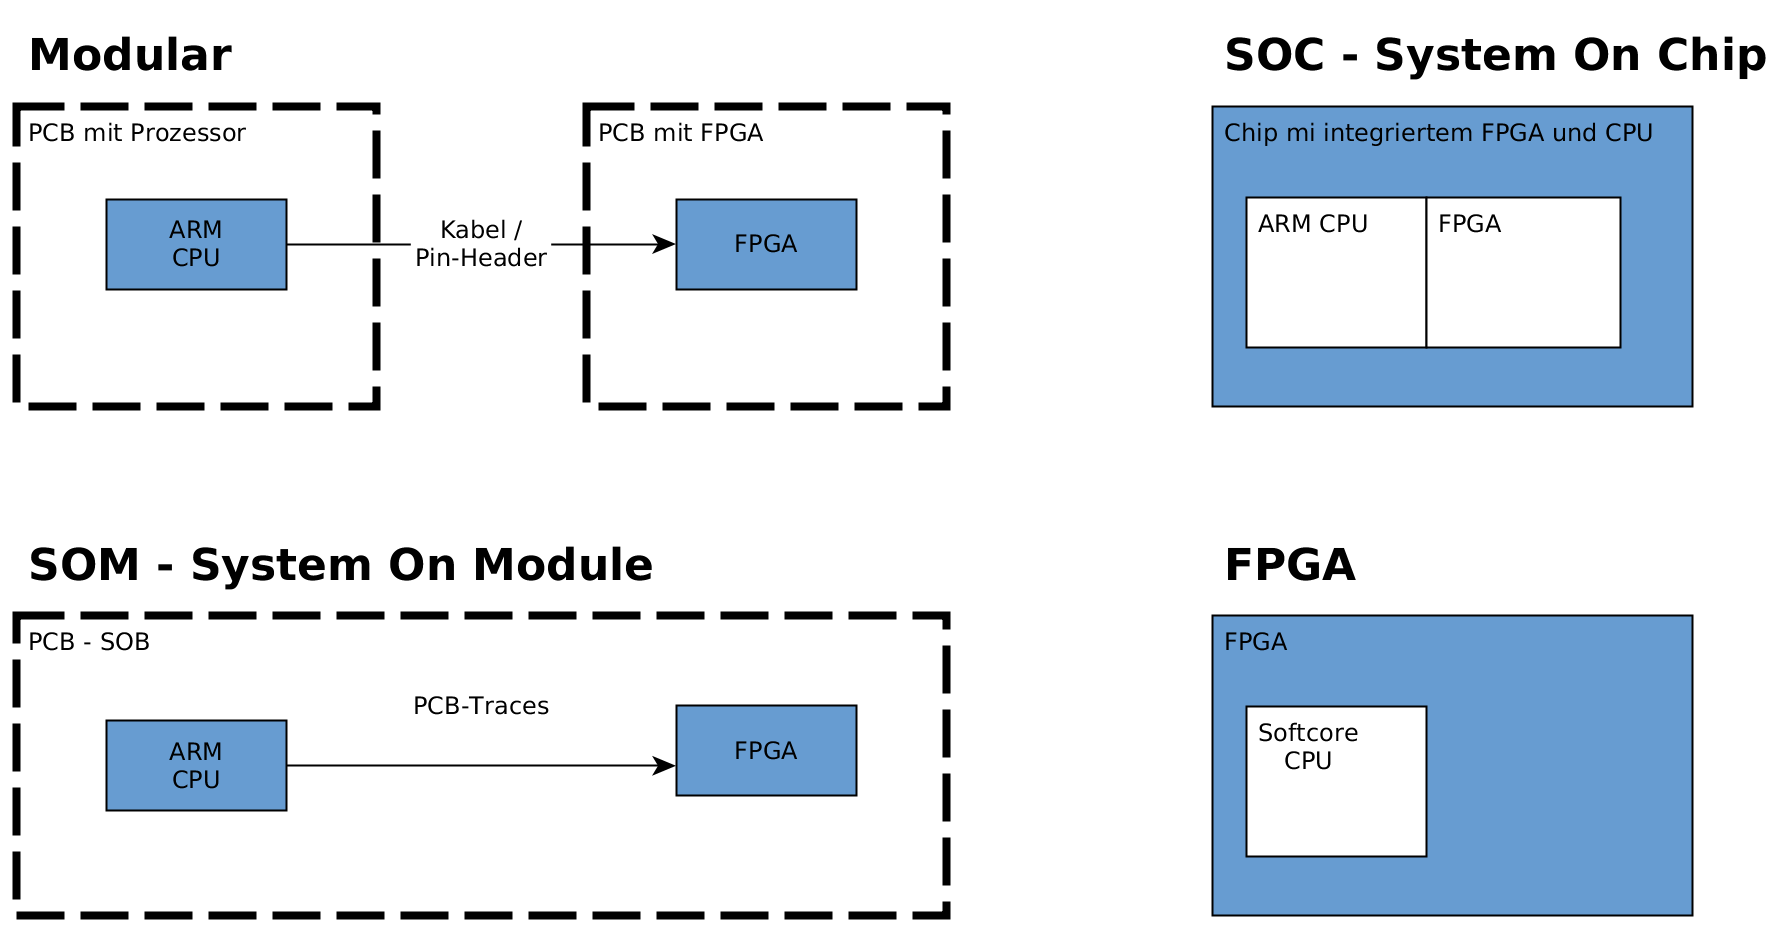
\includegraphics[width=\textwidth,height=\textheight,keepaspectratio]{graphs/bauformen.png}
	\caption[]{Mögliche Anbindungen des FPGA an die CPU}
	\label{fig:anbindungFPG}
\end{figure}
% \FloatBarrier

\subsection{FPGA als Zusatzplatine zum Prozessorboard - Bauweise ''Modular''}
Das \textit{''FPGA Development Board CAPE for the BEAGLEBONE''}\footnote{\ \ Direkter Link: \ \ \ \ \ \ \ \ \ https://www.element14.com/community/docs/DOC-69215/l/fpga-development-board-cape-for-the-beaglebone\\ Archivierter Link: \ \ \ https://web.archive.org/save/https://www.element14.com/community/docs/DOC-69215/l/fpga-development-board-cape-for-the-beaglebone}  ist eine Aufsteckplatine für den \textit{Beaglebone Black}.
Wenn sie auf den \textit{Beaglebone Black} aufgesteckt wird, erweitert sie den ARM-basierten Linux PC um einen \textit{''Spatran 6 LX9''} FPGA, inklusive einiger I/O-Peripherien und SDRAM.

\textit{Vorteile:}
\begin{itemize}
	\item Relativ günstig.
	\item Funktioniert ''Out of the Box''
	\item Schnelles GPMC-Interface (General-Purpose Memory Controller) zwischen Prozessor und FPGA.
\end{itemize}

\textit{Nachteile:}
\begin{itemize}
	\item Verwendet ein modifiziertes Linux-Image, das LOGI-Image.
	\item Der eMMC (Embedded Multi Media Card) Speicher des Beaglebone kann nicht gleichzeitig mit dem GPMC verwendet werden.
	\item Die Verfügbarkeit vom Cape ist nicht garantiert.
	\item Nur ein FPGA und Prozessor erhältlich.
\end{itemize}

Eine modulare Bauweise ist grundsätzlich sehr flexibel.
Leider sind auf dem Markt nur sehr wenige verschiedene Module zu finden.
So ein kleines Angebot disqualifiziert diese Bauweise.


\subsection{FPGA auf dem gleichen Modul wie der Prozessor (System On Module) - Bauweise ''SOM''}
Bei einem SOM (System On Module) ist die CPU und auch der FPGA auf dem gleichen PCB-Modul verbaut.
Dadurch kann der Hersteller auf dem Modul ein Bus mit kontrollierter Impedanz implementieren.
Dies ermöglicht eine sehr hohe Bandbreite bei der Kommunikation zwischen der CPU und dem FGPA.
Das Modul benötigt ein zusätzliches PCB, ein Basisboard, in dem es eingebettet werden kann.
Oft existieren Experimentierboards mit einer grossen Zahl an unterschiedlichen I/O-Möglichkeiten, die gebrauchsfertig gekauft werden können.
Für eine spezifische Anwendung muss ein solches Basisboard für das SOM selbst designed werden, weil ein Experimentierboard oft zu gross ist, oder nicht die benötigte Peripherie enthält.
Da neben dem FPGA auch High-Speed-Peripherie, wie z.B. RAM auf dem Modul verbaut ist, kann beim Basisboard oft auf die aufwändige Entwicklung von High-Speed-PCB-Traces verzichtet werden.


Es hat sich gezeigt, dass es nur zwei Anbieter SOM mit FPGA produzieren.
Nur die beiden Anbieter \textit{solectrix}\footnote{\ \ Direkter Link: \ \ \ \ \ \ \ \ \ https://www.solectrix.de/de/sxom-module\\ Archivierter Link: \ \ \ https://web.archive.org/save/https://www.solectrix.de/de/sxom-module} und \textit{OposSom}\footnote{\ \ Direkter Link: \ \ \ \ \ \ \ \ \ http://www.opossom.com/english/products-processor\_boards-apf6\_sp.html\\ Archivierter Link: \ \ \ https://web.archive.org/save/http://www.opossom.com/english/products-processor\_boards-apf6\_sp.html} scheinen solche Module zu verkaufen.

Weil die Auswahl für SOMs sehr klein ist wurde diese Bauform nicht mehr weiter verfolgt.

 
\subsection{FPGA im gleichen Gehäuse wie der Prozessor (System On Chip) - Bauweise ''SOC''}
Seit einigen Jahren werden Produkte verkauft, die eine programmierbare Logik (FPGA) und auch eine dedizierte CPU in einem Chip-Gehäuse verbaut haben.
Da der FPGA und auch die CPU im selben Gehäuse verbaut sind, ist eine sehr schnelle, integrierte Kommunikation zwischen CPU und FPGA möglich.

Die beiden grossen FPGA-Hersteller Altera und auch Xilinx bieten beide mehrere Produkte als eine SOC Lösung an.
Die Produkte von Altera sind aber deutlich teurer als die Chips von Xilinx.
Besonders die Evaluierungsboards von Altera sind sehr teuer.

Bei der Produktfamilie Zynq von Xilynx gibt es ein breites Angebot von SOCs und auch von Experimentierboards.
Das Experimentierboard \textit{''Zybo''} wird sogar schon im Unterricht der NTB für die Entwicklung von VHDL genutzt.


\subsection{ARM als Softcore in FPGA - Bauweise ''FPGA''}
% TODO0: softcore FPGA
In FPGAs können Prozessoren als sogenannte \textit{Softcores} implementiert werden.
Dabei wird ein Teil der FPGA-Gates so konfiguriert, dass sie wie ein Mikroprozessor verwendet werden können.

Es existieren aber nur Designs für einfachere Mikroprozessoren, da komplexe Prozessoren viel zu viele Gates benötigen, um ökonomisch sinnvoll zu sein.
ARM-Prozessoren der Cortex-A-Familie sind sehr komplex und nicht als FPGA-Softcores erhältlich.
Von der ARM-Cortex-Familie sind nur Cortex-M0 und Cortex-M1 erhältlich.
Diese Cores sind aber kostenpflichtig und nicht Open Source.

Weil keine Cortex-A-Cores erhältlich sind und alle anderen ARM-Cores kostenpflichtig sind, wird diese Bauweise nicht mehr weiter verfolgt.



% \subsubsection{Übersicht Bauformen}
\begin{table}[]
\centering
\begin{tabular}{|l|l|l|}
\hline
\textbf{Bauweise} & \textbf{Vorteile}                                                                                                                      & \textbf{Nachteile}                                                       \\ \hline
\textbf{Modular}  & \begin{tabular}[c]{@{}l@{}}* Günstig wenn nur Prozessor verwendet wird\\ * Unterschiedliche FPGAs können verwendet werden\end{tabular} & \begin{tabular}[c]{@{}l@{}}* Datenbus evt. nicht Memory \\mapped    \end{tabular}                                  \\ \hline
\textbf{SOB}      & \begin{tabular}[c]{@{}l@{}}* Sauberes, abgeschlossenes System\end{tabular} & * FPGA ist fix                                                           \\ \hline
\textbf{SOC}      & \begin{tabular}[c]{@{}l@{}}* Potenziell sehr schnelle Datenverbindung\\ \ \ \ zwischen FPGA und Prozessor\\ * Sauberes, abgeschlossenes System\end{tabular}                       & \begin{tabular}[c]{@{}l@{}}* FPGA ist fix\\ * Relativ teuer\end{tabular} \\ \hline
\textbf{FPGA}     & * Flexibel                                                                                                                             & * Sehr teuer                                                             \\ \hline
\end{tabular}
\label{t-uebersichtBauformen}
\caption{Übersicht Bauformen}
\end{table}

%\section{Cortex-M}
%\textbf{Cortex-M0}
%A very small processor (starting from 12K gates) for low cost, ultra low power microcontrollers and deeply embedded applications
%
%\textbf{Cortex-M0+}
%The most energy-efficient processor for small embedded system. Similar size and programmer’s model to the Cortex-M0 processor, but with additional features like single cycle I/O interface and vector table relocations
%
%\textbf{Cortex-M1}
%A small processor design optimized for FPGA designs and provides Tightly Coupled Memory (TCM) implementation using memory blocks on the FPGAs. Same instruction set as the Cortex-M0
%
%\textbf{Cortex-M3}
%A small but powerful embedded processor for low-power microcontrollers that has a rich instruction set to enable it to handle complex tasks quicker. It has a hardware divider and Multiply-Accumulate (MAC) instructions. In addition, it also has comprehensive debug and trace features to enable software developers to develop their applications quicker
%
%\textbf{Cortex-M4}
%It provides all the features on the Cortex-M3, with additional instructions target at Digital Signal Processing (DSP) tasks, such as Single Instruction Multiple Data (SIMD) and faster single cycle MAC operations. In addition, it also have an optional single precision floating point unit that support IEEE 754 floating point standard
%
%\textbf{Cortex-M7}
%High-performance processor for high-end microcontrollers and processing intensive applications. It has all the ISA features available in Cortex-M4, with additional support for double-precision floating point, as well as additional memory features like cache and Tightly Coupled Memory (TCM)



\subsection{Wahl der Bauweise}
Es hat sich gezeigt, dass es nicht sehr viele Produkte gibt, die einen Cortex-A-Prozessor in Kombination mit einem FPGA bieten.
Einige Produkte zielen mehr auf den Hobby-Bereich, wie zum Beispiel das \textit{''FPGA Development Board CAPE for the BEAGLEBONE''}.
Für professionellere Lösungen scheinen selbstentwickelte PCBs der Standard zu sein.
Alle anderen Ansätze sind oft nur Nischenprodukte für spezielle Anwendungen oder mit geringer Verfügbarkeit.

Seit einigen Jahren ist aber eine signifikante Auswahl von SOCs auf dem Markt.
Diese werden aber nur von den beiden Herstellern Altera und Xilinx angeboten.
Beide Hersteller bieten aber ein sehr umfangreiches Angebot.

% Die SOCs bieten d



\section{Fazit - Auswahl der Hardware}
Da die Wahl bereits auf einen Cortex-A in einem SOC eingeschränkt wurde, ist das verbleibende Angebot sehr begrenzt.
Die Entscheidung zwischen Zynq von Xilinx und den SOCs von Altera fällt auf Zynq, da die Altera Experimentierboards mehrere tausend Franken kosten.

Das Zybo-Experimentierboard ist eine sehr naheliegende Wahl, da es bereits für den Unterricht in der NTB genutzt wird.
Der Preis des Boards ist auch tief genug, dass eine ganze Klasse für den Unterricht damit ausgerüstet werden kann.
Eine grosszügige Auswahl an I/Os bieten eine sehr hohe Flexibilität zum experimentieren und auch für den Unterricht.

Das Zybo ist mit einem Zynq-7000 bestückt.
Der Zynq-7000 ist ein Modell mit einem Dual-Core-Cortex-A9-Prozessor mit 667 MHz.
Es existieren aber auch noch günstigere Zynqs mit weniger Leistung und sehr viel teurere Varianten mit einem leistungsstärkeren Prozessor und grösseren FPGA.
Zusätzlich sind die Zynqs als standalone Chip oder als Modul inklusive RAM erhältlich.

All diese Eigenschaften machen das Zybo mit dem Zynq-7000 zum klaren Favorit.


% TODO bild zybo
	\chapter{Überblick über das ganze System}
Dieses Kapitel bietet eine grobe Übersicht über das ganze System, um die Zusammenhänge zwischen einzelnen Komponenten aufzuzeigen.
Auf einzelne Komponenten und Toolchains wird in den folgenden Kapiteln genauer eingegangen.


\section{Schematische Übersicht}
In Abbildung \ref{fig:UebersichtDebuggerToolchain} ist das ganze System abgebildet.
Das \textit{Zybo} beinhaltet neben dem FT2232-Chip auch noch diverse I/O-Peripherien, die in einer \textit{deep}-Applikation genutzt werden können.
Der FT2232 auf dem \textit{Zybo} übernimmt zwei verschiedene Funktionen.
Einerseits wird er als USB zu UART Brücke (schwarzer Pfeil) verwendet, damit der Windows PC einfach eine serielle Verbindung mit dem Prozessor aufbauen kann, andererseits fungiert er als Brücke zum blauen JTAG-Bus.
Das bedeutet, er erhält Befehle von der OpenOCD-Software über USB und übersetzt diese elektrisch und auch logisch für das JTAG Interface.
OpenOCD ist eine Software-Zwischenschicht die für den Debugger benötigt wird.

Auf dem \textit{Windows PC} wird die \textit{deep}-Applikation in Eclipse geschrieben, kompiliert und debuggt.
Plugins erweitern Eclipse um die notwendigen Funktionen, die für die Entwicklung von \textit{deep}-Applikationen notwendig sind.
In dieser Übersicht sind beide Debug Toolchains, die ''klassische'' Abatron-Toolchain und die neue OpenOCD-Toolchain, abgebildet.

Bei der \textit{Abatron-Toolchain} wird das \textit{Abatron BDI3000} mit dem \textit{abatronInterface}-Plugin über die rote TCP/IP-Verbindung angesprochen.
Das BDI kommuniziert dann über die blaue JTAG-Verbindung direkt mit dem Zynq-Chip.

Die grünen Pfeile zeigen den Kommunikationsweg für die neuen OpenOCD-Toolchains.
OpenOCD bildet zusammen mit der richtigen Hardware, hier ist es der FT2232-Chip, einen kompletten Debugger und ist somit eine Alternative zum BDI3000.
Die OpenOCD-Software stellt einen \textit{gdb}-Server und auch ein CLI (\textit{Command Line Interface}) zur Verfügung.
% referenz zu openOCDInterface
Das neue Eclipse-Plugin \textit{''OpenOCDInterface''} verwendet das CLI über den TCP/IP-Port 4444 (grüner Pfeil) und bildet so die \textit{CLI-OpenOCD-Toolchain}.
OpenOCD verwendet dann den \textit{WinUSB}-Treiber um mit dem FT2232-Chip über USB zu kommunizieren.
Der FT2232-Chip verwendet denselben blauen JTAG-Bus wie das BDI3000 zur Kommunikation mit dem Zynq.

Die \textit{gdb-OpenOCD-Toolchain} kann mit einem allein lauffähigen \textit{gdb} verwendet werden (orange, gestrichelter Pfeil), wie in Kapitel \ref{chapter:Der-gdb-Debugger} beschrieben.
Eine weitere Möglichkeit wäre ein \textit{gdb}-Plugin für Eclipse, damit der \textit{gdb} direkt aus Eclipse heraus verwendet werden kann.
Beide Varianten kommunizieren mit dem \textit{gdb}-Server von OpenOCD über den TCP/IP-Port 3333 (oranger Pfeil).


\begin{figure}[htbp]
	\centering
		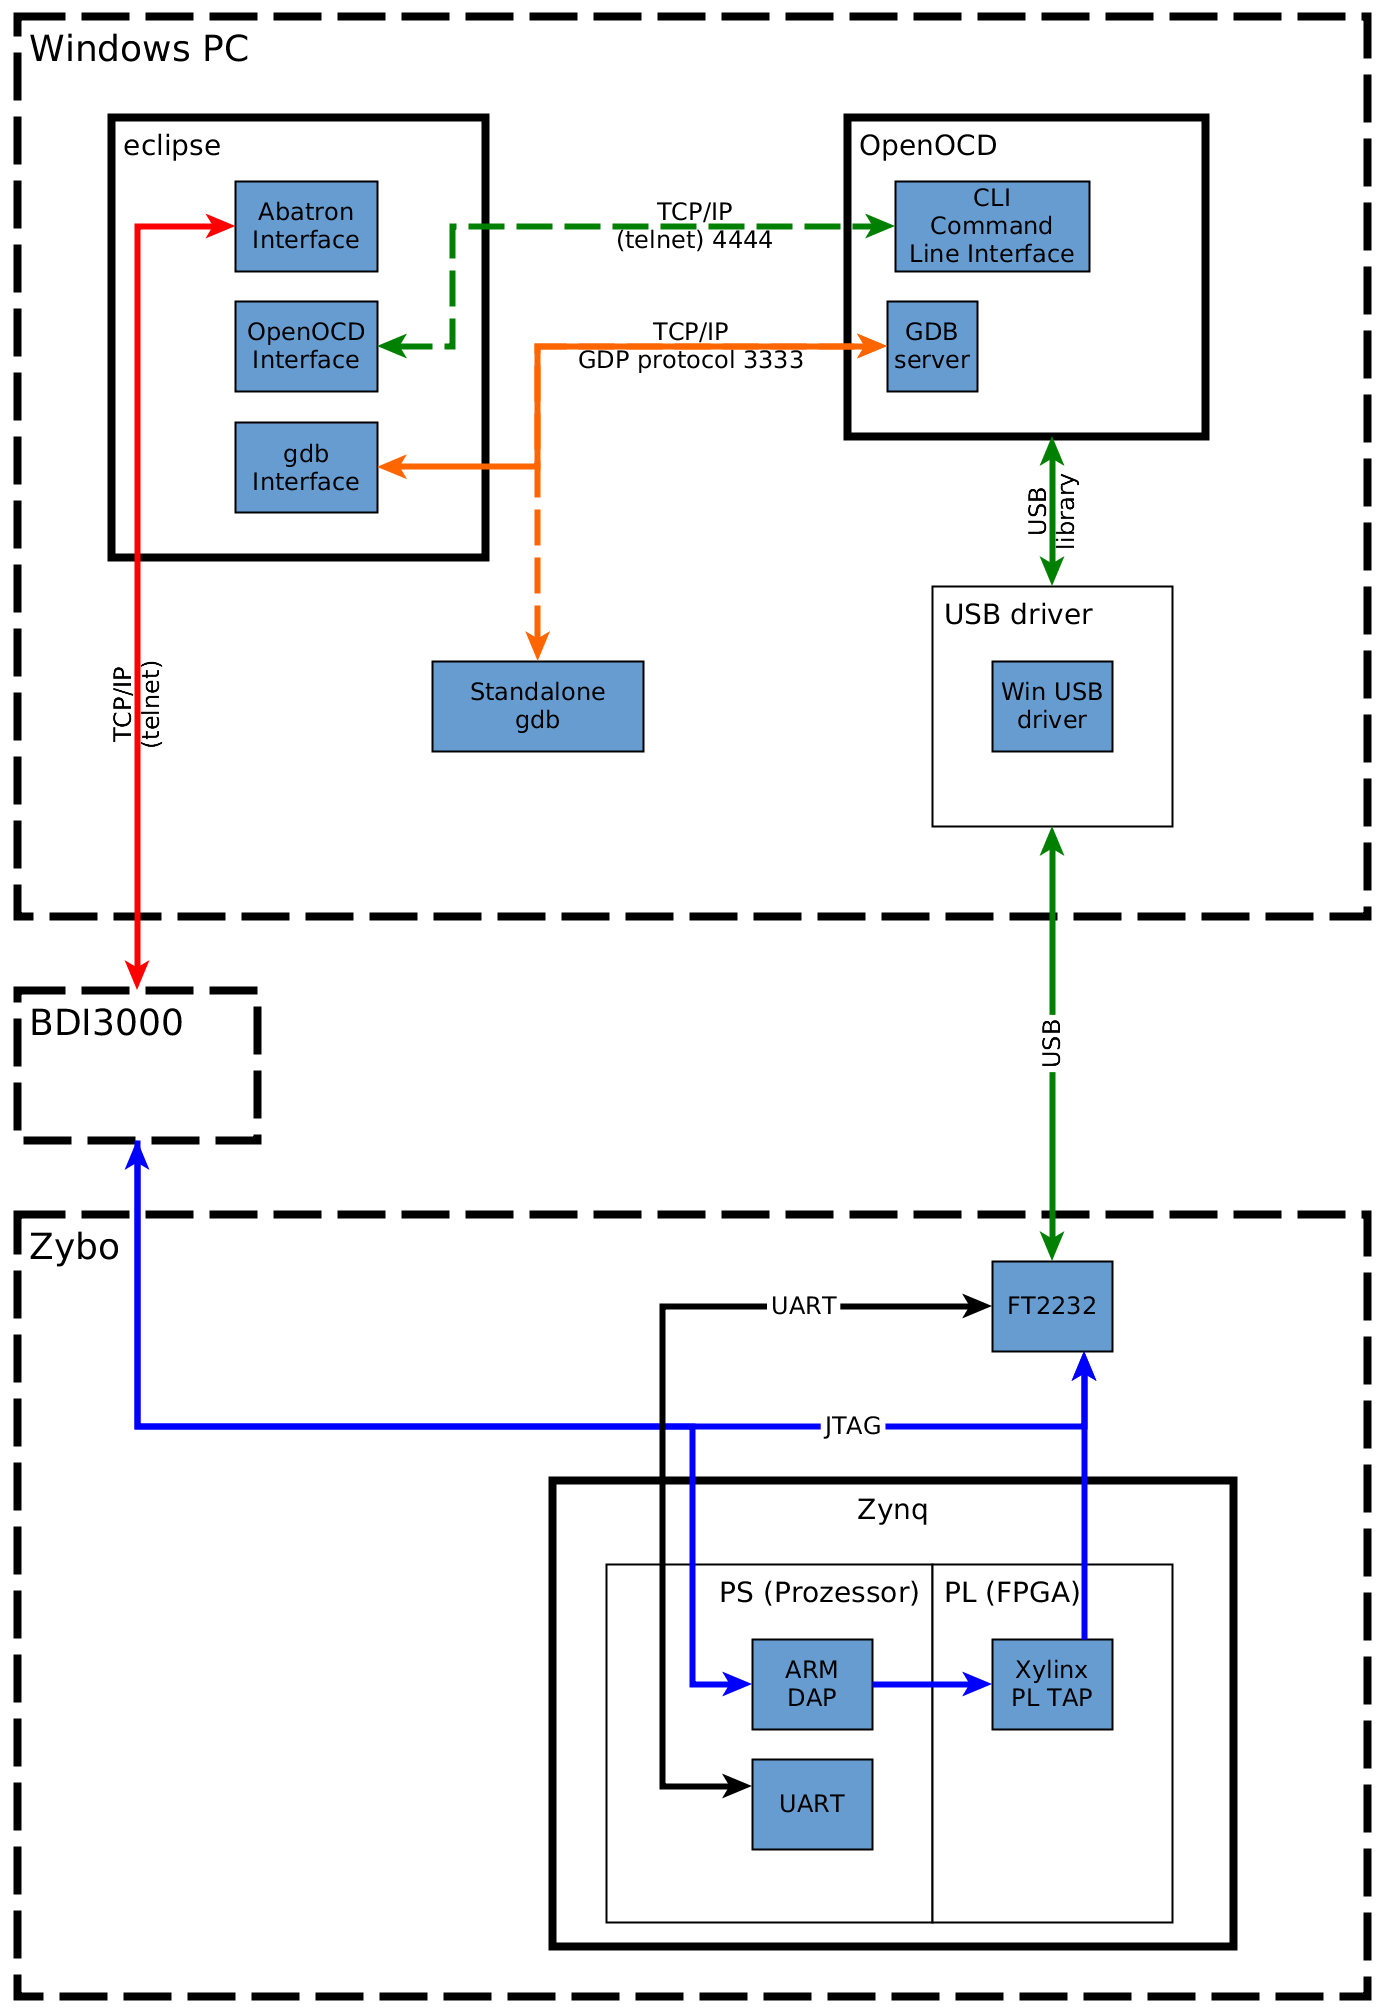
\includegraphics[width=\textwidth,height=\textheight,keepaspectratio]{graphs/embeddedDebuggerToolchain.png}
	\caption{Systemübersicht Debugger Toolchain}
	\label{fig:UebersichtDebuggerToolchain}
\end{figure}



\FloatBarrier
\section{Debugger Toolchains}
Im Folgenden werden die drei verschiedenen Toolchains genauer erklärt.

\subsection{Abatron-Toolchain}
Die \textit{Abatron-Toolchain} (Abbildung \ref{fig:AbatronToolchain}) benötigt weder die OpenOCD-Software noch den FT2232-Chip, dafür aber den teuren BDI3000-Debugger.
Diese ''klassische'' Toolchain nutzt das bestehende \textit{deep}-Plugin \textit{abatronInterface} und wird für die Entwicklung von \textit{deep} für den PowerPC verwendet.
In dieser Arbeit wird die \textit{Abatron-Toolchain} nicht verwendet.

\begin{figure}[htbp]
	\centering
		% 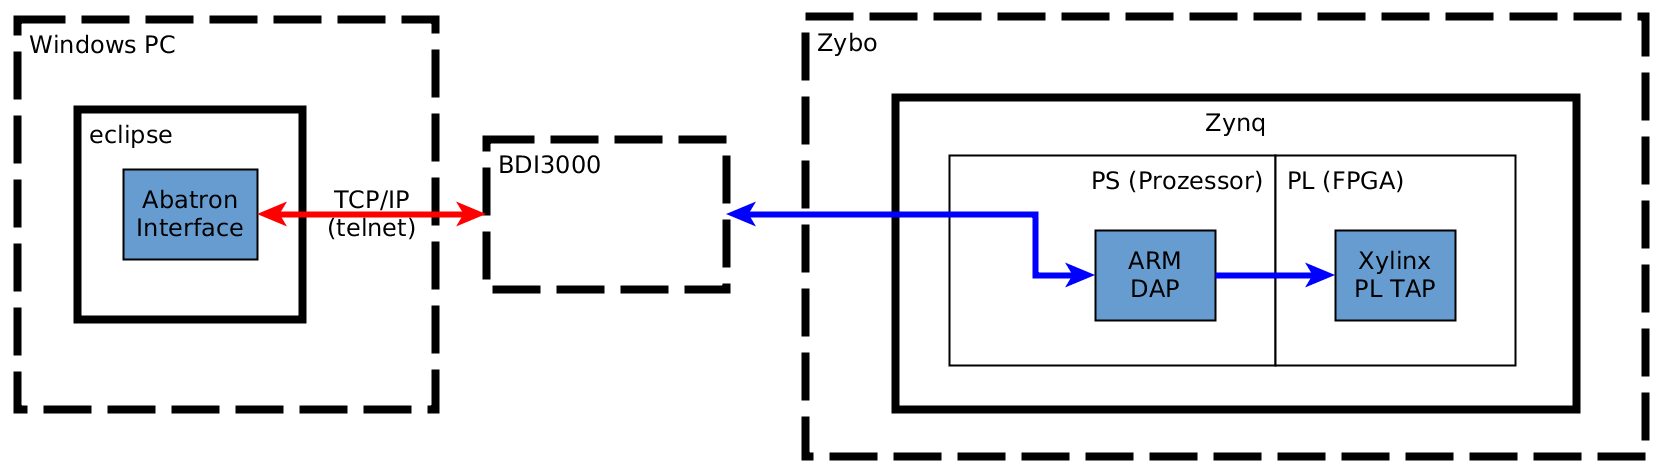
\includegraphics[width=\textwidth,height=\textheight,keepaspectratio]{graphs/abatronToolchain.png}
		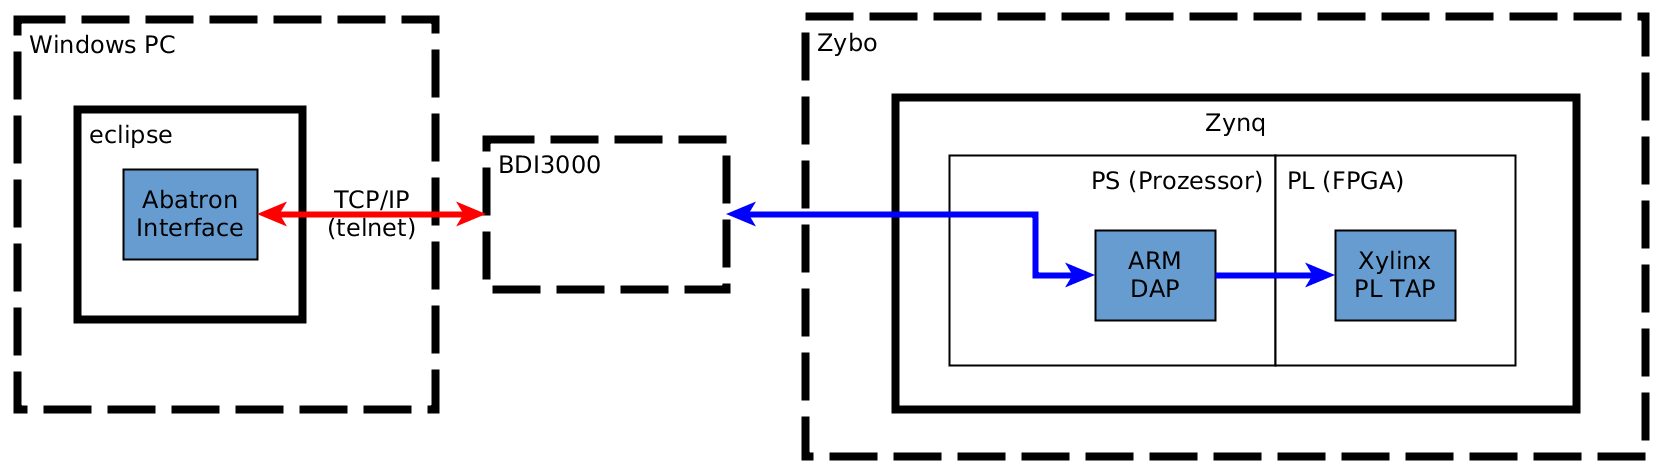
\includegraphics[width=10cm,height=\textheight,keepaspectratio]{graphs/abatronToolchain.png}
	\caption{Abatron-Toolchain}
	\label{fig:AbatronToolchain}
\end{figure}


\FloatBarrier
\subsection{CLI-OpenOCD-Toolchain}
Wie in Abbildung \ref{fig:CLIOpenOCDToolchain} zu sehen ist, wird das teure BDI wird für diese Toolchain nicht  benötigt.
% verbessern: satzbau
Da das CLI (Command Line Interface) von OpenOCD aber sehr ähnlich ist wie das CLI des BDI, ist eine Portierung der bestehenden \textit{Abatron-Toolchain} in die neue \textit{CLI-OpenOCD-Toolchain} relativ einfach.
Die \textit{CLI-OpenOCD-Toolchain} lehnt sich deshalb sehr stark an die bestehende \textit{Abatron-Toolchain} an.
% Die bestehende Toolchain für den PPC ist nicht auf der offiziellen \textit{deep}-Homepage dokumentiert.

Mit dieser Toolchain ist \textit{Sourcecode-Debugging} aber nicht möglich.
Das bedeutet, es ist nicht möglich im Sourcecode Breakpoints zu setzten oder durch einzelne Zeilen im Sourcecode zu steppen.
Bestehende Möglichkeiten aus der alten \textit{Abatron-Toolchain}, wie \textit{''TargetOperations''}, bleiben aber erhalten.

Im Kapitel \ref{section:CLI-OpenOCD-Toolchain} wird die Implementation dieser Toolchain genauer beschrieben.


\begin{figure}[htbp]
	\centering
		% 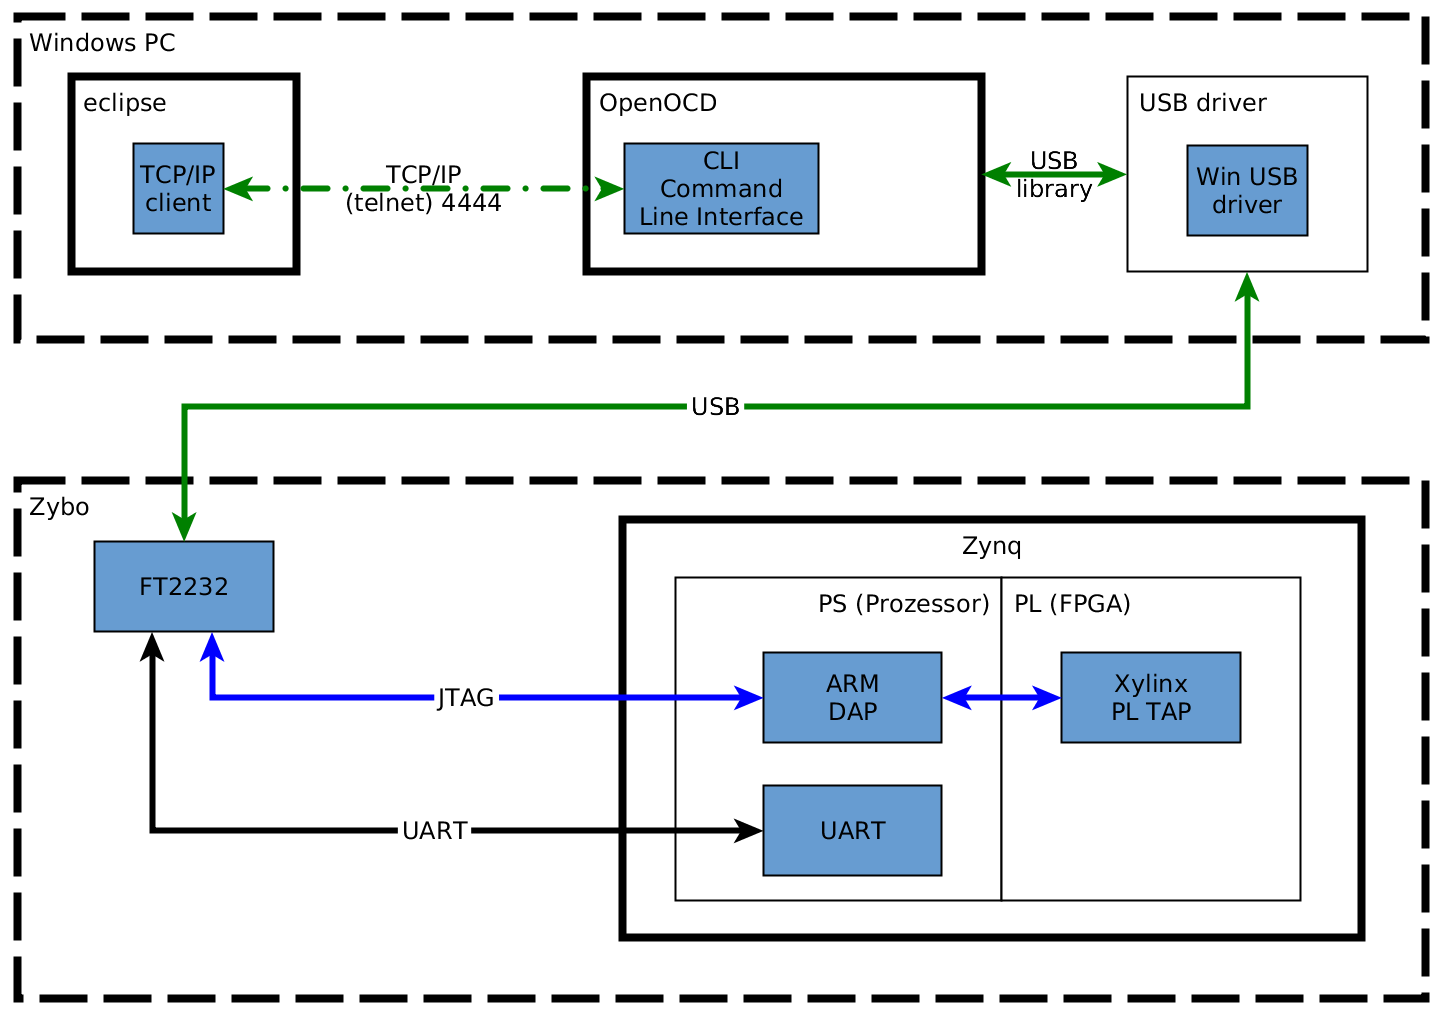
\includegraphics[width=\textwidth,height=\textheight,keepaspectratio]{graphs/CLIOpenOCDToolchain.png}
		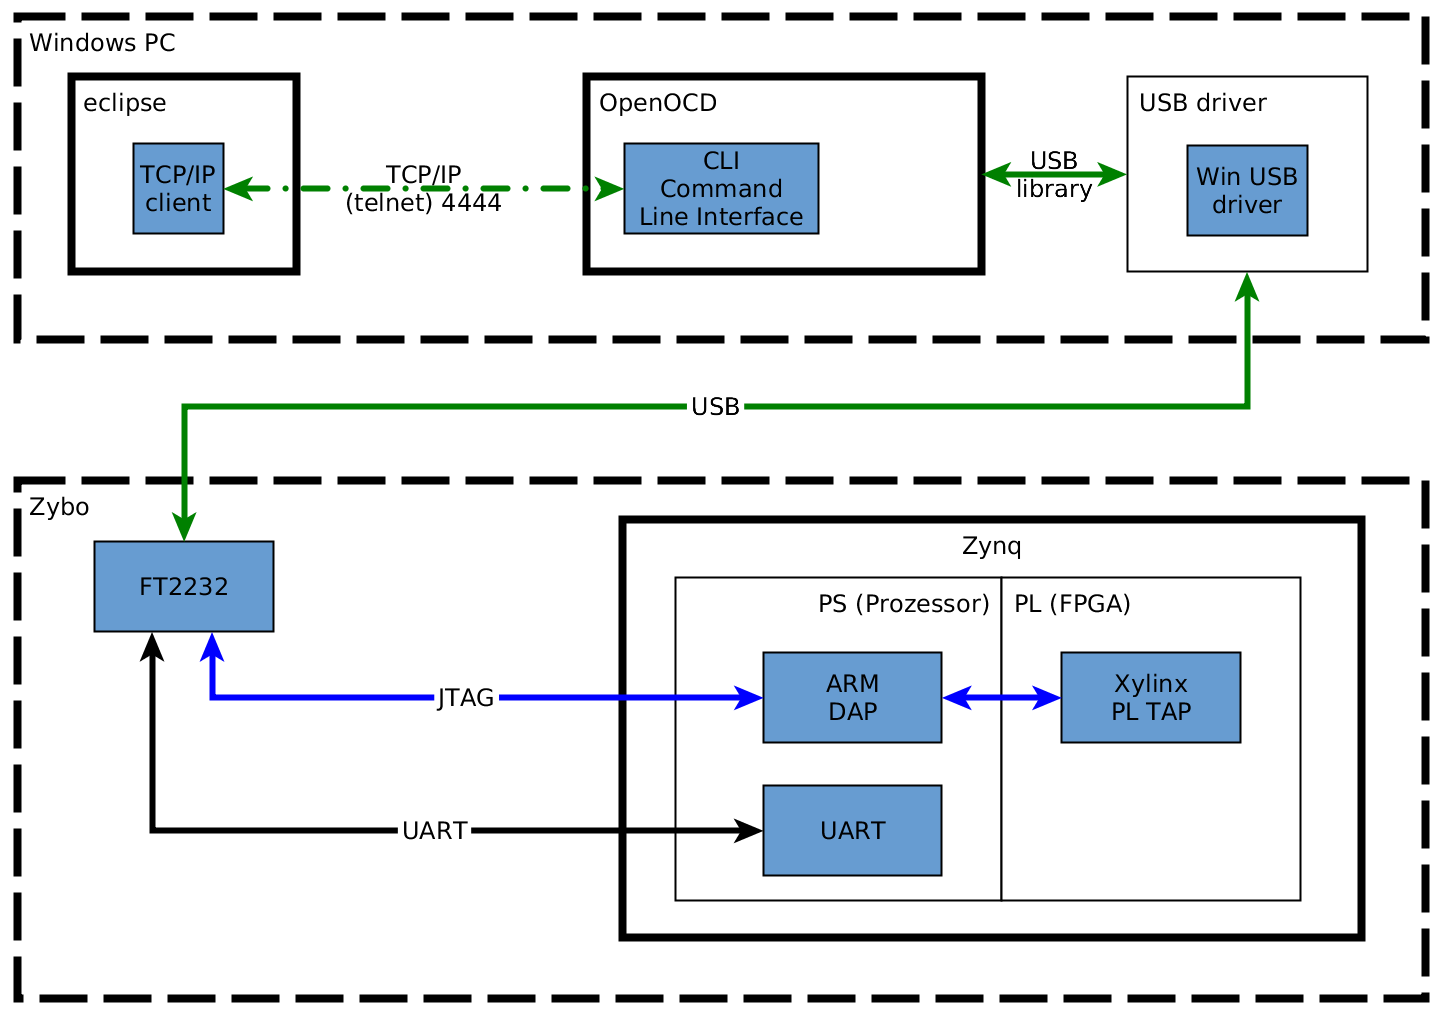
\includegraphics[width=10cm,height=\textheight,keepaspectratio]{graphs/CLIOpenOCDToolchain.png}
	\caption{CLI-OpenOCD-Toolchain}
	\label{fig:CLIOpenOCDToolchain}
\end{figure}


\FloatBarrier
\subsection{\textit{gdb}-OpenOCD-Toolchain}
In der \textit{gdb-OpenOCD-Toolchain} wird, wie bei der obigen Toolchain, ebenfalls die OpenOCD-Software und der FT2232-Chip verwendet.
Es wird aber nicht mehr ein Interface bestehend auf der ''klassischen'' Abatron Toolchain verwendet, sondern es wird direkt das CLI des \textit{gdb}-Debugger genutzt.
In der schematischen Übersicht der Toolchain in Abbildung \ref{fig:gdbOpenOCDToolchain} wird deutlich, dass sie fast die gleichen Komponenten nutzt wie die \textit{CLI-OpenOCD-Toolchain}.
% Dadurch kann \textit{Sourcecode-Debugging} direkt in Eclipse eingesetzt werden.
Mit dem \textit{gdb} können auch erweiterte Debugging-Featurers wie \textit{Sourcecode-Lookup} und \textit{Breakpoints} verwendet werden.
% günstige hardware

In dieser Arbeit wird nur die vereinfachte Toolchain mit dem Standalone-\textit{gdb}-Debugger implementiert.
Mit der vereinfachten Toolchain kann das CLI des \textit{gdb} in Kombination mit der \textit{OpenOCD-Toolchain} für zum Debuggen genutzt werden.

Die komplette \textit{gdb-OpenOCD-Toolchain} kann auf dieser Toolchain aufbauen.
Bei der kompletten \textit{gdb-OpenOCD-Toolchain} soll der \textit{gdb} im Eclipse integriert werden.
Dadurch kann in Eclipse die Applikation entwickelt und auch debuggt werden.

Im Kapitel \ref{chapter:Der-gdb-Debugger} wird diese Toolchain detailliert beschrieben.


\begin{figure}[htbp]
	\centering
		% 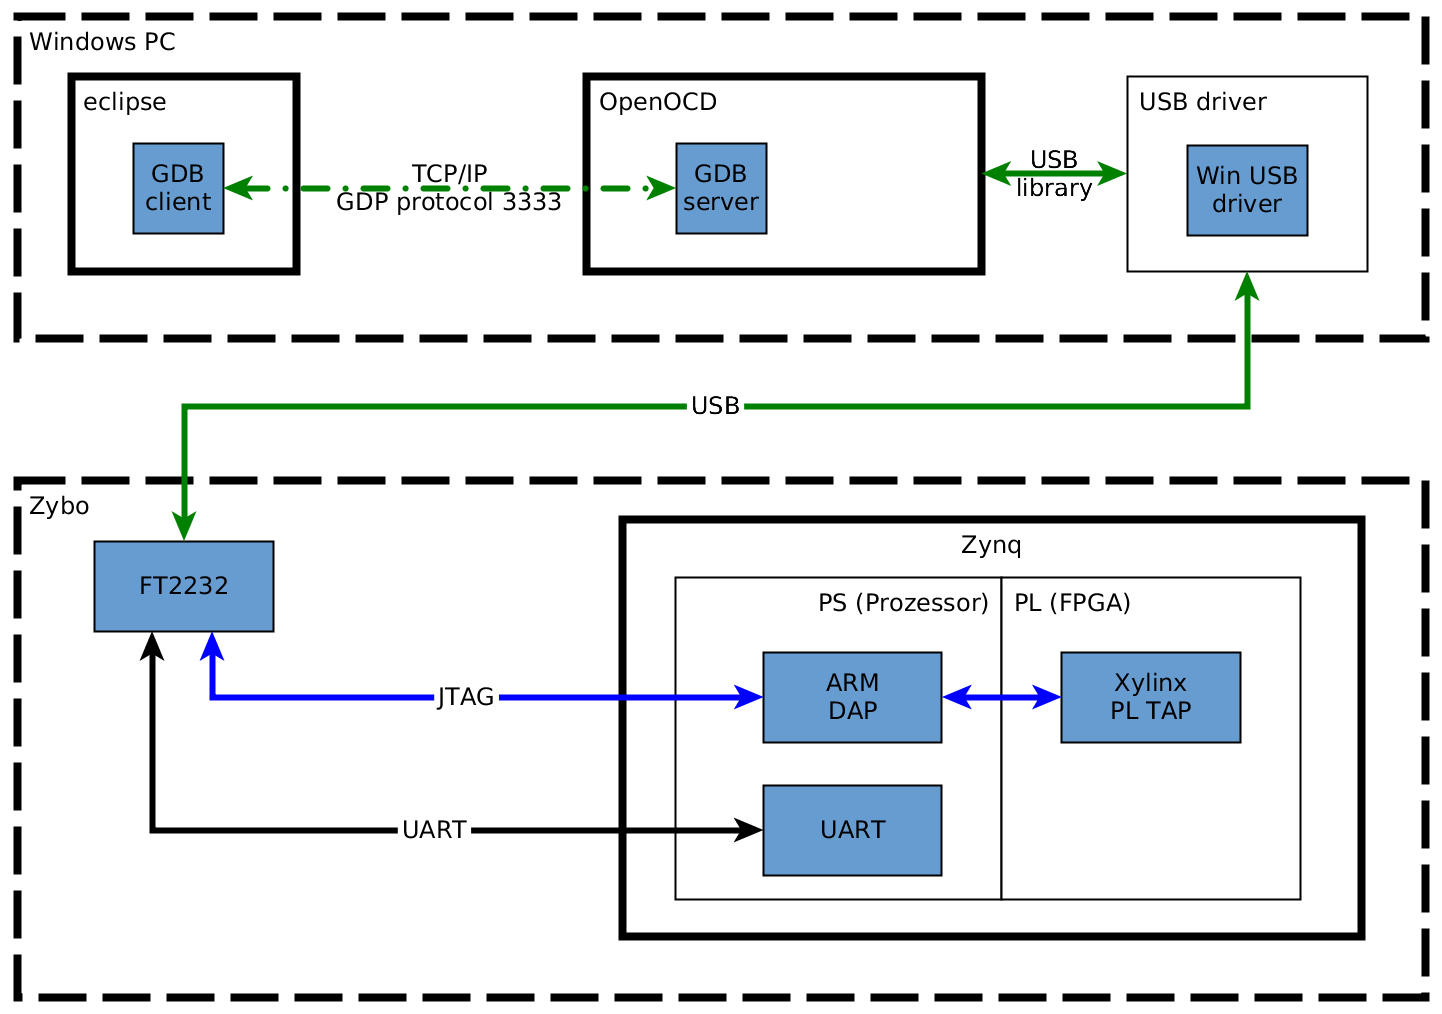
\includegraphics[width=\textwidth,height=\textheight,keepaspectratio]{graphs/gdbOpenOCDToolchain.png}
		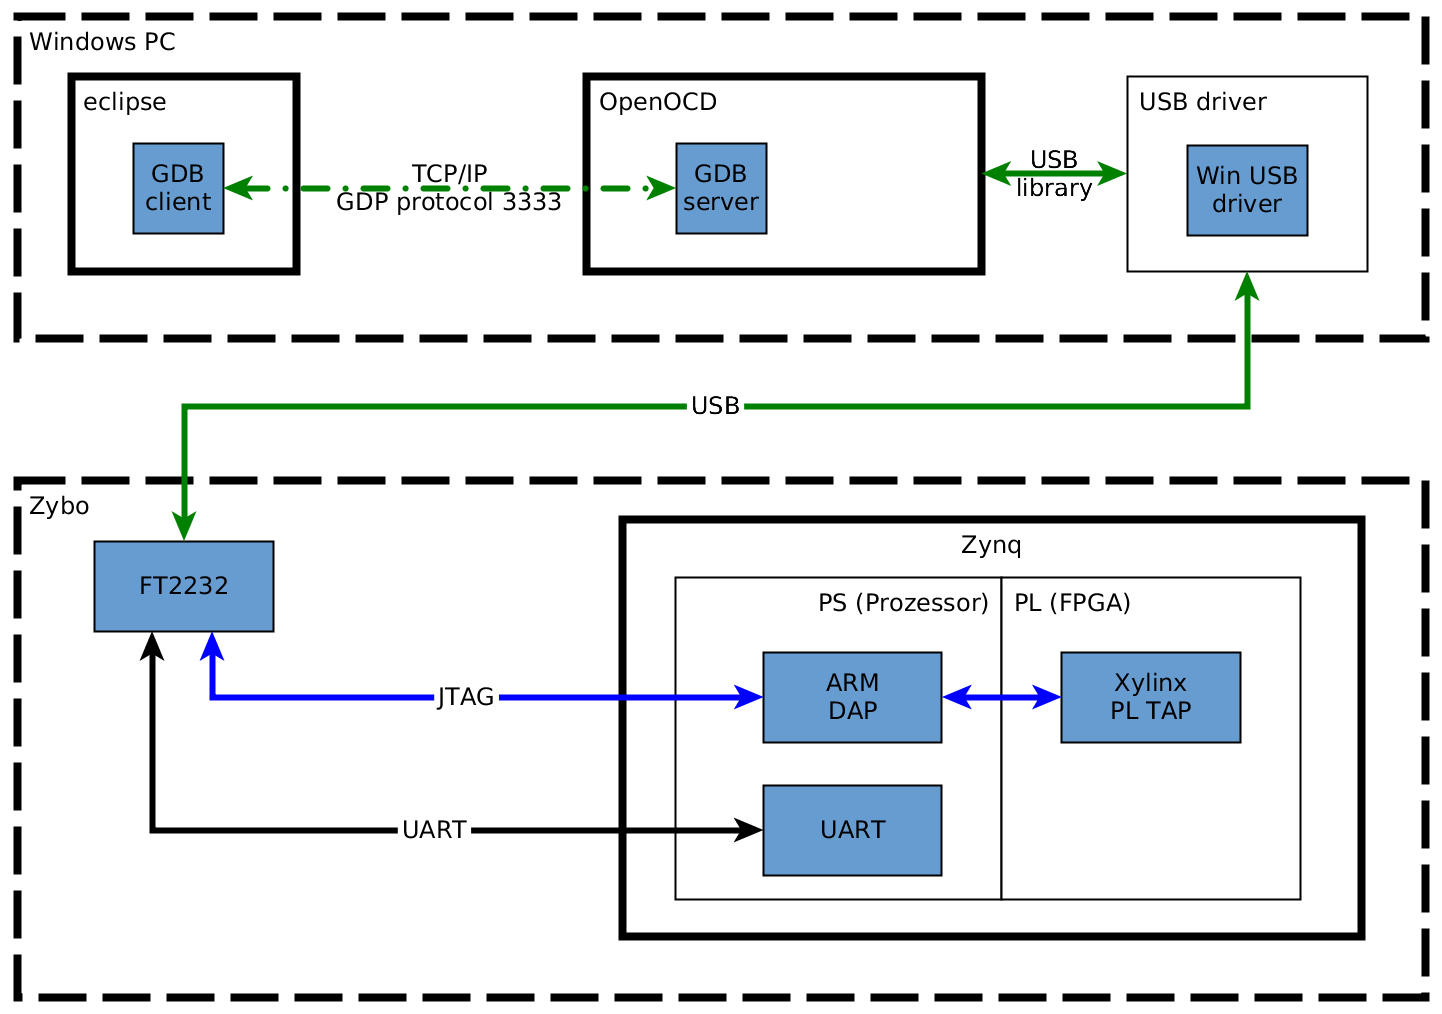
\includegraphics[width=10cm,height=\textheight,keepaspectratio]{graphs/gdbOpenOCDToolchain.png}
	\caption{\textit{gdb}-OpenOCD-Toolchain}
	\label{fig:gdbOpenOCDToolchain}
\end{figure}
	% TODO: Kapitel unterkapitel

\chapter{Zynq}
Der Zynq-7000 ist ein SoC (System on Chip), das einen 667 MHz Dual-Core ARM Cortex-A9 Prozessor und eine programmierbare Logik enthält, die einem Artix-7 FPGA entspricht.
Der Prozessor und dessen Peripherie befindet sich im \textit{Processing System} oder kurz PS.
Der FPGA-Teil des Zynq wird oft PL oder \textit{Programmable Logic} genannt.
Über den internen AMBA-Bus kann der Prozessor und auch die PL auf die Peripherie, wie z.B. SPI, GPIO, Ethernet oder auch DDR3, zugreifen.
Das Block Diagramm in der Abbildung \ref{fig:BlockDiagrammZynq} gibt einen guten Überblick über das ganze SoC.
Das restliche Kapitel beschreibt relevante Komponente und Eigenarten des Zynq.

\begin{figure}[htbp]
	\centering
		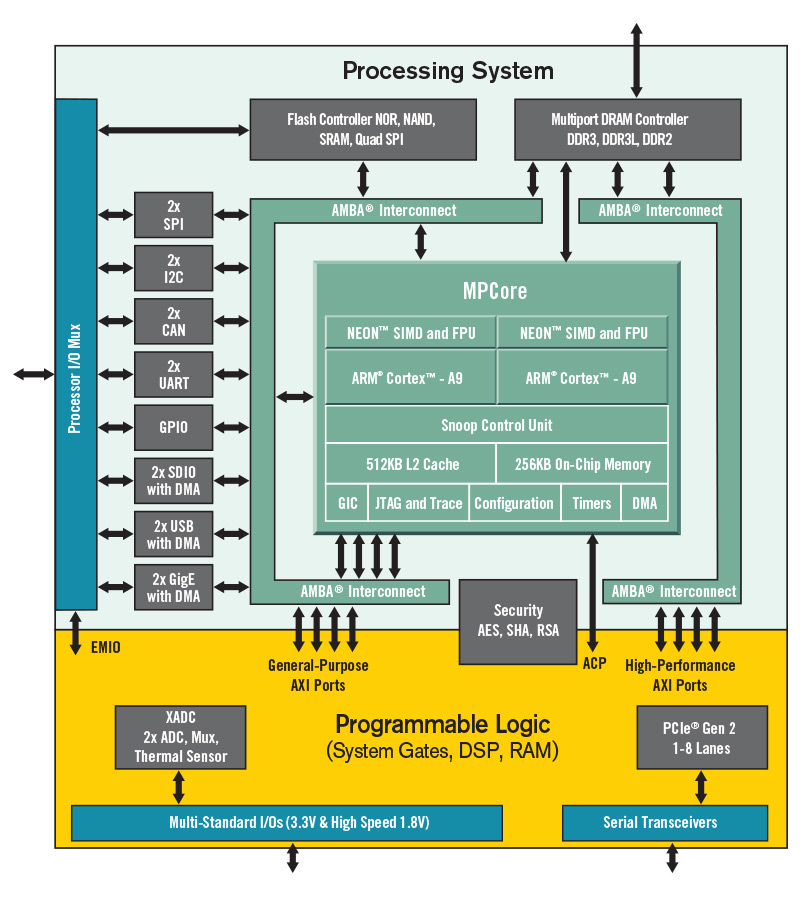
\includegraphics[width=10cm,height=\textheight,keepaspectratio]{images/zynqBlockDiagram.png}
	\caption[Block Diagramm Zynq\-7000]{Block Diagramm Zynq\-7000\footnotemark}
	\label{fig:BlockDiagrammZynq}
\end{figure}
\footnotetext{https://www.xilinx.com/products/silicon-devices/soc/zynq-7000.html}


\section{MIO und EMIO}
MIOs sind \textit{Multiplexed Input Output Pins}, welche direkt vom Prozessor angesprochen werden können, ohne dass die PL programmiert werden muss.
Die EMIOs sind \textit{\textbf{Extended} Multiplexed Input Output Pins}, welche nur über die PL angesprochen werden können.
Aus diesem Grund können die EMIOs nur verwendet werden, wenn die PL entsprechend programmiert wurde.
Diese Arbeit beschränkt sich nur auf die MIOs und das PS.
Im TRM\footnote{Technical Reference Manual} des Zynq\cite{bib:ZynqTechnicalReferenceManual} im Kapitel \textit{''2.5.4 MIO-at-a-Glance Table''} ist eine sehr gute Übersicht über alle möglichen Funktionen der MIOs gegeben.

% TODO MIO config des zybos

\section{Standard Zybo Workflow}
Im \textit{Getting Started with Zynq\footnote{https://reference.digilentinc.com/learn/programmable-logic/tutorials/zybo-getting-started-with-zynq/start?redirect=1}} Tutorial von Digilent ist beschrieben, wie man ein einfaches Design für die PL und ein einfaches Programm für das PS erstellt.
Das Tutorial deckt den ganzen Workflow ab.
Dabei werden, z.B. für LED1, LED2 und LED3, auch die EMIOs verwendet.
In Schritt 1 bis 7 wird mit Vivado das Design für die PL erstellt und exportiert.

\textbf{Hinweis1:} Die Zybo Toolchain benötigt den standard USB-Treiber. Im Kapitel \ref{kapitel:usbTreiber} ist beschrieben, wie der standard USB-Treiber wieder installiert werden kann.

\textbf{Hinweis2:} Vivado und die Xilinx SDK müssen für dieses Tutorial installiert sein.

Ab Schritt 8 wird beschrieben, wie im XSDK (\textit{Xilinx Standard Development Kit}) ein einfaches ''Hello World'' Programm in C für den Prozessor geschrieben werden kann.
% Das XSDK ist Eclipse mit einem Xilinx Plug-In.

Das XSDK verwendet im Hintergrund das XSCT\footnote{https://www.xilinx.com/html\_docs/xilinx2018\_1/SDK\_Doc/xsct/intro/xsct\_introduction.html} (\textit{Xilinx Software Command-Line Tool}).
Das XSDK kann interaktiv, oder mit Scripts verwendet werden.
% Die Scriptsprache basiert, wie auch Jim-TCL, auf der Sprache TCL.
Wie Jim-TCL basiert auch die verwendete Scriptsprache auf der Sprache TCL.
Wird das ''Hello World'' Programm im XSDK gestartet, erscheint im \textit{SDK Log} Fenster ein detailliertes Log des ausgeführten Scripts.
In diesem Log kann nachvollzogen werden, was das Script beim Download und Start des Programms alles ausgeführt hat.

% TODO was auch immer
Im Anhang \ref{anhang:SDKLog} ist eine Kopie eines solchen Logs zu finden.
% TODO: langesWort
% \textit{D:/Vivado/01\_gettingStarted/01\_gettingStarted.sdk/.sdk/launch\_scripts/xilinx\_c-c++\_application\_(system\_debugger)/system\_debugger\_using\_debug\_01\_gettingstarted\_applicationproject.elf\_on\_local.tcl}
% \textit{D:/Vivado\01\_gettingStarted\01\_gettingStarted.sdk\.sdk\launch\_scripts\xilinx\_c-c++\_application\_(system\_debugger)\system\_debugger\_using\_debug\_01\_gettingstarted\_applicationproject.elf\_on\_local.tcl}

Das Script \textit{ps7\_init.tcl} definiert unter anderem die fünf Initialisierungs-Methoden:
\begin{itemize}
%\begin{itemize}
\item \textit{ps7\_mio\_init\_data\_3\_0}
\item \textit{ps7\_pll\_init\_data\_3\_0}
\item \textit{ps7\_clock\_init\_data\_3\_0} 
\item \textit{ps7\_ddr\_init\_data\_3\_0}
\item \textit{ps7\_peripherals\_init\_data\_3\_0}
\end{itemize}
Die Initialisierungs-Methoden werden in der Methode \textit{ps7\_init} aufgerufen.
\textit{ps7\_init} wiederum wird in Zeile 8 des \textit{...elf\_on\_local.tcl} Scripts aufgerufen, welches beim Start des ''Hello World'' Programms im XSDK ausgeführt wird.
In Zeile 9 vom \textit{...elf\_on\_local.tcl} wird auch die Methode \textit{ps7\_post\_config} von \textit{ps7\_init.tcl} aufgerufen, welche im Anschluss \textit{ps7\_post\_config\_3\_0} aufruft.

Alle Konfigurationsregister sind im Anhang B vom \textit{Zynq TRM}\cite{bib:ZynqTechnicalReferenceManual} beschrieben.
Bevor die Register aber verändert werden können, müssen sie \textit{''unlocked''} werden, in dem der Wert \textit{0x0000DF0D} in die Adresse \textit{0xF8000008} geschrieben wird.


\subsection{Grundlegende Methoden}
Alle Methoden des \textit{ps7\_init.tcl}-Scripts sind auf den folgenden vier Grundbefehlen aufgebaut:\\
\textbf{mwr -force <address> <value>: }\\
Schreibt den Wert <value> in die Adresse <address>.

\textbf{mask\_write <address> <mask> <value>: }\\
Schreibt die Bits der Maske <mask> von <value> in die Addresse <address>.

\textbf{mask\_poll <address> <mask>:  }\\
Wartet, bis die maskierten Bits <mask> des Speicherinhalts von der Speicheradresse <address> gleich 0 sind.

\textbf{mask\_dellay <address> <value>:}\\
Wartet <value> Millisekunden.

% TODO silikon version überprüfen ps7_init.tcl.745


\subsection{Initialisierungsmethoden}
\label{Initialisierungsmethoden}
Im Folgenden werden alle Methoden beschrieben, welche zur Initialisierung des Zynq auf dem Zybo verwendet werden.

\textbf{ps7\_mio\_init\_data\_3\_0:}\\
Diese Methode initialisiert die MIOs.
Der Multiplexer für die IO Pins wird konfiguriert.
Dadurch wird definiert, welcher Pin von welcher Peripherie, wie UART und auch RAM, verwendet wird.
Zusätzlich werden auch, falls vorhanden, folgende elektrischen Charakteristiken definiert:
\begin{itemize}
\item \textbf{Pullup:} Pullup Widerstand aktivieren / deaktivieren.
\item \textbf{IO\_Type:} Buffer Type: LVCMOS 1.8V, LVCMOS 2.5V, LVCMOS 3.3V,  oder HSTL.
\item \textbf{Speed:} Slow oder fast CMOS edge.
\item \textbf{Tristate:} Enalbe / disable Tristate.
\end{itemize} 


\textbf{ps7\_pll\_init\_data\_3\_0}\\
Initialisiert die drei PLLs\footnote{Phase Locked Loop} ARM, DDR und IO.
Bei jeder PLL-Initialisierung wird darauf gewartet, bis der PLL betriebsbereit (locked) ist.
Die Dauer dieser Wartezeit ist unbekannt.

\textbf{ps7\_clock\_init\_data\_3\_0}\\
Konfiguriert diverse Clocks, die im Prozessor gebraucht werden.

\textbf{ps7\_ddr\_init\_data\_3\_0}\\
Konfiguriert den DDR Bus.
Für die Konfiguration werden insgesamt 79 verschiedene Register geschrieben und die DCI (\textit{Digital Controlled Impedance}) kalibriert.
Nachdem diese Methode ausgeführt wurde, kann der DDR genutzt werden.
Vorher ist nur der OCM (On Chip Memory) nutzbar.
Mehr dazu im Kapitel \ref{MemoryMapping}.

\textbf{ps7\_peripherals\_init\_data\_3\_0}\\
Konfiguriert folgende Peripherien:
\begin{itemize}
\item UART1
\item QSPI (für Flash Speicher auf Zybo)
\item POR timer
\item High-Low-Wait(1msec)-High Sequenz für MIO46 (USB-OTG Ping)
\end{itemize}  




Die oben genannten Initialisierungsfunktionen werden vom Xilinx Debugger jedesmal ausgeführt, wenn die Applikation im XSDK mit \textit{''Launch on Hardware (System Debuger)''} gestartet wird.
Es ist aber auch möglich, die Initialisierung direkt mit der C-Applikation und nicht mit dem Debugger durchzuführen.
Wird die Initialisierung in der Applikation durchgeführt, und die Applikation auf dem Flash Speicher des Zynq gespeichert, dann Initialisiert sich der Zynq bei jedem Start selber.
Im Beispielprogramm \textit{''helloworld.c''} ist die Methode \textit{''init\_platform()''} enthalten, welche in \textit{''platform.c''} deklariert ist.
Standardmässig ist die darin enthaltene Methode \textit{''ps7\_init()''} aber auskommentiert.
\textit{''platform.c''} befindet sich im \textit{''design\_wrapper\_hw\_platform''}, welcher in Vivado erzeugt wurde.
Vergleicht man \textit{''ps7\_init()''} mit \textit{ps7\_init.tcl}, dann sieht man schnell, dass das Script und auch die C-Methode genau die gleichen Register schreiben und lesen.

\textit{''psu\_init()''} ist für ein \textit{''Zynq UltraScale+™ MPSoC''} Chip, welcher auf dem Zybo nicht verwendet wird.


\textit{Auszug aus ''helloworld.c'' (Komplettes Programm im Anhang \ref{anhang:helloworld.c}):}
\lstset{language=c}
\begin{lstlisting}[frame=single]
...
#include "platform.h"
..
int main ()
{
...
init_platform();

while(1){
...
\end{lstlisting}



\textit{Auszug aus ''platform.c'' (Komplettes Programm im Anhang \ref{anhang:platform.c}):}
\lstset{language=c}
\begin{lstlisting}[frame=single]
...
/*#include "ps7_init.h"*/
/*#include "psu_init.h"*/
...
void
init_platform()
{
    /*
     * If you want to run this example outside of SDK,
     * uncomment one of the following two lines and also #include "ps7_init.h"
     * or #include "ps7_init.h" at the top, depending on the target.
     * Make sure that the ps7/psu_init.c and ps7/psu_init.h files are included
     * along with this example source files for compilation.
     */
    /* ps7_init();*/
    /* psu_init();*/
    enable_caches();
    init_uart();
}
...

\end{lstlisting}




\subsection{ps7\_init.tcl Script für OpenOCD anpassen}
Da das \textit{ps7\_init.tcl} Script ebenfalls auf der TCL-Sprache basiert, kann es gut für OpenOCD angepasst werden.
Einige Methoden werden aber nur vom XSCT unterstützt und nicht von OpenOCD.
Mit folgenden Änderungen ist das Script mit OpenOCD kompatibel:

\begin{enumerate}
\item Untenstehende Methoden wurden dem Script hinzugefügt.

\textit{Auszug aus ''ps7\_init\_modified.tcl'' (Komplettes Script im Anhang \ref{anhang:ps7initmodified.tcl}):}
\lstset{language=tcl}
\begin{lstlisting}[frame=single]
proc unlock_SLCR {} {
	mww 0xF8000008 0x0000DF0D
}

proc map_OCM_low {} {
	unlock_SLCR
	mww 0xF8000910 0x00000010
}

proc memread32 {ADDR} {
    set foo(0) 0
    if ![ catch { mem2array foo 32 $ADDR 1  } msg ] {
	return $foo(0)
    } else {
	error "memread32: $msg"
    }
}

proc mask_write { addr mask val } {
	set curval [memread32 $addr]
	set maskinv [expr {0xffffffff ^ $mask}]
    set maskedcur [expr {$maskinv & $curval}]
	set maskedval [expr {$mask  & $val}]
    set newval [expr $maskedcur | $maskedval]
	mww $addr $newval
}

proc initPS {} {
	ps7_init
	ps7_post_config
}
\end{lstlisting}

\item Jeder \texttt{''mwr -force <address> <value>''} Befehl wurde mit \texttt{''\textbf{mww} <address> <value>''} ersetzt.

\item Folgende Methoden wurden mit den untenstehenden Implementationen ersetzt.

% TODO highlight changed lines
\textit{Auszug aus ''ps7\_init\_modified.tcl'' (Komplettes Script im Anhang \ref{anhang:ps7initmodified.tcl})}:
\lstset{language=tcl}
\begin{lstlisting}[frame=single]
proc mask_poll { addr mask } {
    set count 1
    % set curval [memread32 $addr]
    (*@  \textcolor{blue}{ set curval [memread32 $addr] }  @*)
    set maskedval [expr {$curval & $mask}] # & = bitwise AND
    while { $maskedval == 0 } {
		set curval [memread32 $addr]
        set maskedval [expr {$curval & $mask}]
        set count [ expr { $count + 1 } ]
        if { $count == 100000000 } {
          puts "Timeout Reached. Mask poll failed at ADDRESS: $addr MASK: $mask"
          break
        }
    }
}

proc mask_delay { addr val } {
    set delay  [ get_number_of_cycles_for_delay $val ]
    perf_reset_and_start_timer
    set curval [memread32 $addr]
    set maskedval [expr {$curval < $delay}]
    while { $maskedval == 1 } {
        set curval [memread32 $addr]
        set maskedval [expr {$curval < $delay}]
    }
    perf_reset_clock 
}

proc ps7_post_config {} {
        ps7_post_config_3_0   
}

proc ps7_init {} {
	halt
	ps7_mio_init_data_3_0
	ps7_pll_init_data_3_0
	ps7_clock_init_data_3_0
	ps7_ddr_init_data_3_0
	ps7_peripherals_init_data_3_0
	puts "PCW Silicon Version : 3.0"
}

proc get_number_of_cycles_for_delay { delay } {
  # GTC is always clocked at 1/2 of the CPU frequency (CPU_3x2x)
  set APU_FREQ  650000000
  return [ expr ($delay * $APU_FREQ /(2 * 1000))]
}
\end{lstlisting}

\end{enumerate}


% % TODO implementierung in openOCD scripts



\section{Memory Mapping}
\label{MemoryMapping}
Im Kapitel 4.1 des \textit{Zynq TRM}\cite{bib:ZynqTechnicalReferenceManual} ist der Aufbau des Speichers beschrieben.
Die Abbildung \ref{fig:AddressMapZynq} zeigt einen guten Überblick über die ganzen 4 GB des Adressraumes.
Bei der Map fällt auf, dass nur ca. 1 GB für DDR RAM verwendet werden kann.

Der OCM (\textit{On Chip Memory}) ist ein kleiner Speicher im Zynq der ohne Initialisierung verwendet werden kann. 
Ideal für ein Bootloader.
Für den OCM stehen ganz am Anfang des Speicherbereichs (\textit{0x0000\_0000}) und ganz am Ende (\textit{0xFFFC\_0000}) 256 kB zur Verfügung.
Der OCM besteht aus 4 x 64 kB grossen Teilbereichen, die dem Register \textit{0xF8000910} wahlweise im oberen oder im unteren Bereich zugewiesen werden können.
Beim Bootvorgang werden die ersten drei Teile in den unteren Bereich (\textit{0x0000\_0000 - 0x0002\_FFFF}) und der vierte Teil in den obersten Bereich (\textit{0xFFFF\_0000 - 0xFFFF\_FFFF}) gemapt.
Das geschieht noch bevor die erste Instruktion aus dem User-Code ausgeführt wird, also auch vor dem selbstgeschriebenen Bootloader.
Der oben beschriebene Bootvorgang kann nicht geändert werden.
Mit Pull-Up-Widerständen kann aber beeinflusst werden, ob der ARM im \textit{Secure-Mode} oder im \textit{Non-Secure-Mode} booten soll und wo der Bootloader gesucht werden soll.
Mehr dazu im Zynq TRM\cite{bib:ZynqTechnicalReferenceManual} im Kapitel \textit{''Kapitel 4.4: Boot and Configuration''}.

Der Speicherbereich für den RAM ist erst nutzbar, wenn der RAM initialisiert wurde.
Die Initialisierungsmethode wird im Kapitel \ref{Initialisierungsmethoden}.

\begin{figure}[htbp]
	\centering
		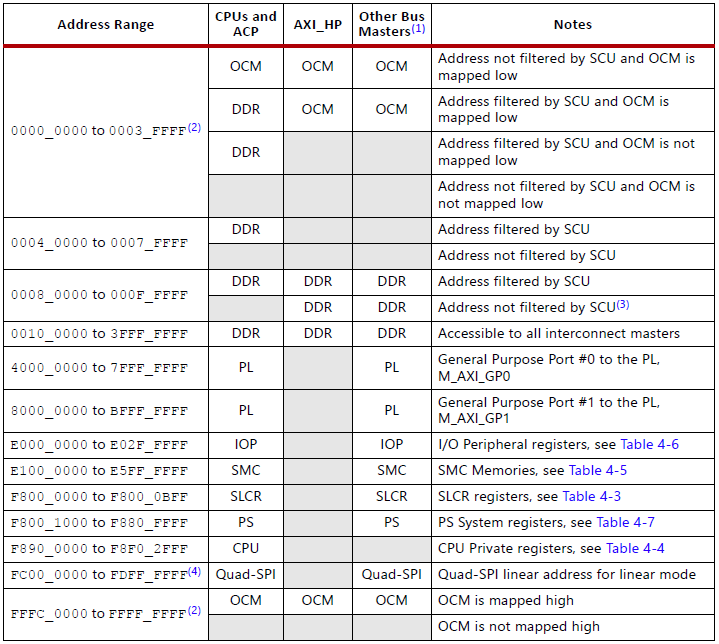
\includegraphics[width=14cm,height=\textheight,keepaspectratio]{images/AddressMapZynq.png}
	\caption[]{Address Map des Zynq}
	\label{fig:AddressMapZynq}
\end{figure}


\section{Floating Point Unit}
FPUs (\textit{Floating Point  Unit}) können je nach Implementation unterschiedliche Funktionen unterstützen.
In den Registern MVFR0 und MVFR (\textit{Media and VFP Feature Register}) lässt sich auslesen welche Funktionen in der Hardware implementiert wurden und genutzt werden können.
Diese Register können aber nicht mit einer einfachen \textit{Memory read} gelesen werden.
Um diese Register oder die anderen speziellen FPU-Register, wie FPSID, FPSCR und PFEXC, lesen zu können, muss die ARM-Instruktion \textit{''VMRS''} verwendet werden.

\subsection{FPU initialisieren}
Damit auf die FPU zugegriffen werden kann, muss der Co-Prozessor 15 erst so konfiguriert werden, dass das System im \textit{secure} und im \textit{non-secure mode} Zugriff auf die FPU hat.
Der CP15 ist ein \textit{''System control coprocessor''}, der neben der FPU auch den Cache und die MPU (Memory Protection Unit) konfiguriert.
Um in ein Register des Co-Prozessors schreiben zu können, muss eine spezielle Instruktion \texttt{''MCR''} verwendet werden, die ein ARM-Register in ein Co-Prozessor-Register speichert.
Da OpenOCD diese Instruktion unterstützt, können die \textit{Access Control Register} direkt mit dem Debugger gesetzt werden.

Das NSACR (\textit{Non-secure Access Control Register}) kontrolliert, ob die FPU auch im \textit{non-secure mode} genutzt werden kann.
Das CPACR (\textit{Coprocessor Access Control Register)} kontrolliert den Zugang zu allen Coprozessoren (CP10 und CP11 sind die FPU).

Zusätzlich muss auch noch das FPEXC EN Bit im FPEXC Register (\textit{Floating-Point Satus and Control Register}) gesetzt werden.
Das FPEXC Register kann aber nicht mit dem Debugger direkt gesetzt werden, da eine spezielle ARM Instruktion dafür verwendet werden muss.
Im Kapitel \textit{''2.4.2 Accessing the FPU registers} des FPU-TRM\cite{bib:FPUTechnicalReferenceManual} sind die Details beschrieben, welche Register genau gesetzt werden müssen.

Mit dem folgenden ARM Code kann die FPU z.B. beim Booten des Kernels initialisiert werden:

\lstset{language=[x86masm]Assembler}
\begin{lstlisting}[frame=single]
; Set bits [11:10] of the NSACR for access to CP10 and CP11 from both Secure and Non-secure states:
MRC p15, 0, r0, c1, c1, 2
ORR r0, r0, #2_11<<10 ; enable fpu/neon
MCR p15, 0, r0, c1, c1, 2
; Set the CPACR for access to CP10 and CP11:
LDR r0, =(0xF << 20)
MCR p15, 0, r0, c1, c0, 2
; Set the FPEXC EN bit to enable the FPU:
MOV r3, #0x40000000
VMSR FPEXC, r3
\end{lstlisting}


\subsection{MVFR lesen mit OpenOCD}
OpenOCD kann zwar direkt die Register der generischen Co-Prozessoren lesen und schreiben, nicht aber die Register der FPU.
Der folgende Ablauf ermöglicht es aber trotzdem, diese Register auszulesen:

\begin{enumerate}
\item OpenOCD starten und für das CLI eine Telnetverbindung zu Port 4444 aufbauen
\item \texttt{reset init}\ \ \ \ \ \textcolor{darkgreen}{// Reset und Initialisierung des ganzen Systems.} 
\item \texttt{arm mcr 15 0 1 1 2 0x0c00}\ \ \ \ \ \textcolor{darkgreen}{// Non-secure access für FPU (NSACR Register).} 
\item \texttt{arm mcr 15 0 1 0 2 0x00f00000}\ \ \ \ \ \textcolor{darkgreen}{// Genereller Zugang für FPU erlauben (CPACR Register).} 
\item \texttt{mww 0x0 0xEEF70A10}\ \ \ \ \ \textcolor{darkgreen}{// Speichert die Instruktion \texttt{''VMRS R0, MVFR0''} in den OCM.}
\item \texttt{mww 0x4 0xEEF61A10}\ \ \ \ \ \textcolor{darkgreen}{// Speichert die Instruktion \texttt{''VMRS R1, MVFR1''} in den OCM.}
\item \texttt{bp 0x8 1 hw}\ \ \ \ \ \textcolor{darkgreen}{// Breakpoint nach der Instruktion (32 Bit Instruktion = 4 Byte)}
\item \texttt{resume 0x0}\ \ \ \ \ \textcolor{darkgreen}{// Führt die Instruktion bei der Adresse 0 aus}
\item \texttt{reg 0}\ \ \ \ \ \textcolor{darkgreen}{// Liest dass Register 0 aus, welches eine Kopie des MVFR0 enthält.}
\item \texttt{reg 1}\ \ \ \ \ \textcolor{darkgreen}{// Liest dass Register 1 aus, welches eine Kopie des MVFR1 enthält.}
\end{enumerate}

Die Inhalte der Register sind:
\begin{itemize}
	\item MVFR0:	0x1011\_0222
	\item MVFR1:	0x0111\_1111
\end{itemize}



\subsection{Unterstützte Features der FPU}
Die Register MVFR0 und MVFR1 enthalten Informationen über die unterstützten Features der FPU.
Auf der Seite B5-36 des ARMv7-A ARM\cite{bib:ARMv7ArchitectureReferenceManual} (\textit{Architecture Reference Manual}) ist beschrieben, wie die unterstützten Features aus den Registern gelesen werden können.

Der Zynq des Zybo unterstützt:
\begin{itemize}
	\item All rounding modes
	\item VFP squarde root operations
	\item VFP divide operations
	\item Full VFP douple-precision v3 (VFPv3)
	\item VFPv3 single-precision
	\item Advanced SIMD register bank: 32 x 64-bit registers
	\item All VFP instructions (\texttt{LDC, STC, MCR,} and \texttt{MRC})
	\item Half-precision floating-point conversion operations (VFP and advanced SIMD)
	\item Single-precision floating-point operations (advanced SIMD)
	\item Integer operations (advanced SIMD)
	\item Load/store operations (advanced SIMD)
	\item Propagation of NaN values
\end{itemize}

Nicht unterstützt wird:
\begin{itemize}
	\item VFP short vectors
	\item VFP exception trapping
\end{itemize}






%	\chapter{Zybo}
\section{Zynq}
\subsection{Übersicht}
Der Zynq-7000 ist ein SoC\footnote{System on Chip} der einen 667 MHz Dual-Core ARM Cortex-A9 Prozessor und einem programmierbare Logik enthält, die einem Artix-7 FPGA entspricht.
Der Prozessor und dessen Peripherie befindet sich im \textit{Processing System} oder kurz PS.
Der FPGA-Teil des Zynq wird oft PL oder \textit{Programmable Logic} genannt.
Über den AMBA-Bus kann der Prozessor und auch die PL auf die Peripherie, wie z.B. SPI, GPIO, Ethernet oder auch DDR3 zugreifen.
Das Block Diagramm in der Abbildung \ref{fig:BlockDiagrammZynq} gibt einen guten Überblick über das ganze SoC.

\begin{figure}[htbp]
	\centering
		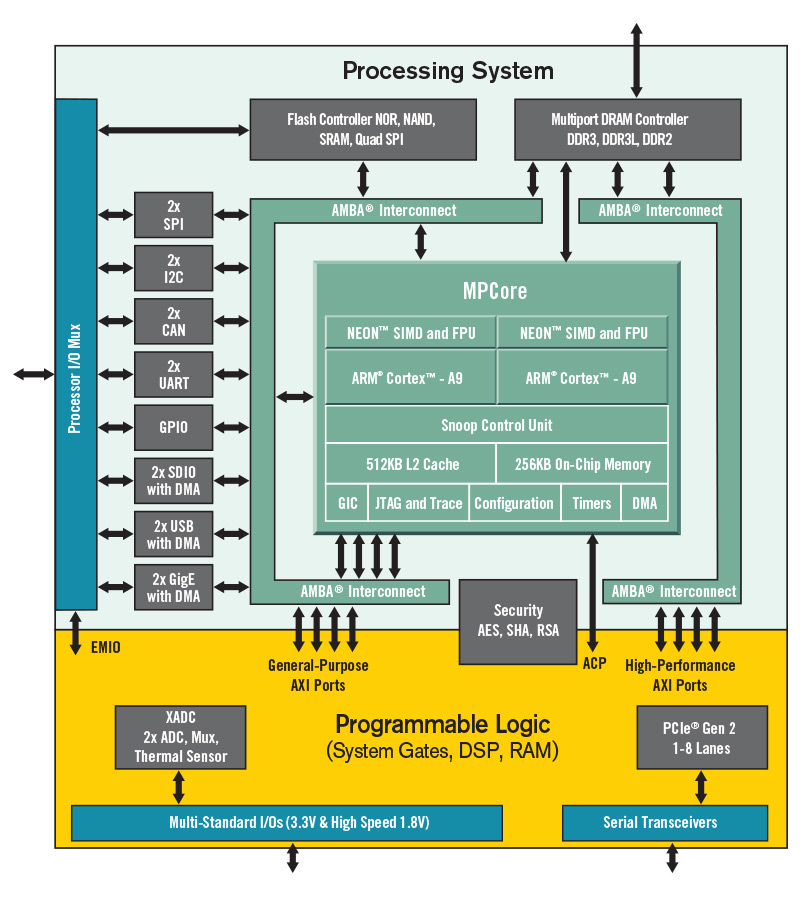
\includegraphics[width=10cm,height=\textheight,keepaspectratio]{images/zynqBlockDiagram.png}
	\caption[Block Diagramm Zynq\-7000]{Block Diagramm Zynq\-7000\footnotemark}
	\label{fig:BlockDiagrammZynq}
\end{figure}
\footnotetext{https://www.xilinx.com/products/silicon-devices/soc/zynq-7000.html}


\subsection{MIO und EMIO}
MIOs sind \textit{Multiplexed Input Output Pins} welche direkt vom Prozessor angesprochen werden können, ohne dass die PL programmiert werden muss.
Die EMIOs sind \textit{\textbf{Extended} Multiplexed Input Output Pins} welche direkt an die PL angeschlossen sind.
Aus diesem Grund können die EMIOs nur verwendet werden, wen die PL entsprechend programmiert wurde.
Diese Arbeit beschränkt sich nur auf die MIOs und das PS.
Im TRM\footnote{Technical Reference Manual} des Zynq\cite{bib:ZynqTechnicalReferenceManual} im Kapitel \textit{''2.5.4 MIO-at-a-Glance Table''} ist eine sehr gute Übersicht über alle möglichen Funktionen der MIOs gegeben.

% TODO MIO config des zybos

\section{Standard Zybo Workflow}
Im \textit{Getting Started with Zynq\footnote{https://reference.digilentinc.com/learn/programmable-logic/tutorials/zybo-getting-started-with-zynq/start?redirect=1}} Tutorial von Digilent ist beschrieben, wie man ein einfaches Design für die PL und ein einfaches Programm für das PS erstellt.
Das Tutorial deckt den ganzen Workflow ab.
Dabei werden, z.B. für LED1 bis LED3, auch die EMIOs verwendet.
In Schritt 1 bis 7 wird mit Vivado das Design für die PL erstellt und exportiert.

\textit{Hinweis1:} Die Zybo Toolchain benötigt den standard USB Treiber. Im Kapitel \ref{kapitel:usbTreiber} ist beschrieben, wie der standard USB Treiber wieder installiert werden kann.

\textit{Hinweis2:} Vivado und die Xilinx SDK müssen für dieses Tutorial installiert sein.

Ab Schritt 8 wird beschrieben, wie im XSDK (\textit{Xilinx Standard Development Kit}) ein einfaches ''Hello World'' Programm in C für den Prozessor geschrieben werden kann.
% Das XSDK ist Eclipse mit einem Xylinx Plug-In.

Das XDSK verwendet im Hintergrund das XSCT\footnote{https://www.xilinx.com/html\_docs/xilinx2018\_1/SDK\_Doc/xsct/intro/xsct\_introduction.html} (\textit{Xilinx Software Command-Line Tool}).
Das XDSK kann interaktiv, oder mit Scripts verwendet werden.
% Die Scriptsprache basiert, wie auch Jim-TCL, auf der Sprache TCL.
Wie auch Jim-TCL basiert die verwendete Scriptsprache auf der Sprache TCL.
Wird das ''Hello World'' Programm im XSDK gestartet, erhält man im \textit{SDK Log} Fenster ein detailliertes Log des ausgeführten Script.
In diesem Log kann nachvollzogen werden, was das Script beim Download und Start des Programms alles ausgeführt.

% TODO was auch immer
Im Anhang \ref{anhang:SDKLog} ist eine Kopie eines solchen Logs zu finden.
% langesWort
\textit{D:/Vivado/01\_gettingStarted/01\_gettingStarted.sdk/.sdk/launch\_scripts/xilinx\_c-c++\_application\_(system\_debugger)/system\_debugger\_using\_debug\_01\_gettingstarted\_applicationproject.elf\_on\_local.tcl}
% \textit{D:/Vivado\01\_gettingStarted\01\_gettingStarted.sdk\.sdk\launch\_scripts\xilinx\_c-c++\_application\_(system\_debugger)\system\_debugger\_using\_debug\_01\_gettingstarted\_applicationproject.elf\_on\_local.tcl}

Das Script \textit{ps7\_init.tcl} definiert unter anderem die fünf Initialisierungs-Methoden:
\begin{itemize}
%\begin{itemize}
\item \textit{ps7\_mio\_init\_data\_3\_0}
\item \textit{ps7\_pll\_init\_data\_3\_0}
\item \textit{ps7\_clock\_init\_data\_3\_0} 
\item \textit{ps7\_ddr\_init\_data\_3\_0}
\item \textit{ps7\_peripherals\_init\_data\_3\_0}
\end{itemize}
Die Initialisierungs-Methoden werden in der Methode \textit{ps7\_init} aufgerufen.
\textit{ps7\_init} wiederum wird in Zeile 8 des \textit{...elf\_on\_local.tcl} Scripts aufgerufen, welches beim Start des ''Hello World'' Programm im XSDK ausgeführt wird.
In Zeile 9 vom \textit{...elf\_on\_local.tcl} wird auch noch die Methode \textit{ps7\_post\_config} von \textit{ps7\_init.tcl} auf, welche im Anschluss \textit{ps7\_post\_config\_3\_0} aufruft.

Alle Konfigurationsregister sind im Anhang B vom \textit{Zynq TRM}\ref{bib:ZynqTechnicalReferenceManual} beschrieben.
Bevor die Register aber verändert werden können, müssen sie \textit{''unlocked''} werden, in dem der Wert \textit{0x0000DF0D} in die Adresse \textit{0xF8000008} geschrieben wird.

Alle Methoden sind auf den folgenden vier Grundbefehlen aufgebaut:\\
\textbf{mwr -force <address> <value>: }\\
Schreibt den Wert <value> in die Adresse <address>.

\textbf{mask\_write <address> <mask> <value>: }\\
Schreibt die Bits der Maske <mask> von <value> in die Addresse <address>.

\textbf{mask\_poll <address> <mask>:  }\\
Wartet bis die maskierten Bits <mask> des Speicherinhalt von der Speicheradresse <address> gleich 0 sind.

\textbf{mask\_dellay <address> <value>:}\\
Wartet <value> Millisekunden.

% TODO silikon version überprüfen ps7_init.tcl.745


\textbf{ps7\_mio\_init\_data\_3\_0:}\\
Diese Methode initialisiert die MIOs.
Es wird der Multiplexer für die IO Pins konfiguriert.
Dadurch wird definiert, welcher Pin von welcher Peripherie, wie UART und auch RAM, verwendet wird.
Zusätzlich werden auch, falls vorhanden, folgende elektrischen Charakteristiken definiert:
\begin{itemize}
\item \textbf{PULLUP:} Pullup Widerstand aktivieren / deaktivieren.
\item \textbf{IO\_Type:} Buffer Type: LVCMOS 1.8V, LVCMOS 2.5V, LVCMOS 3.3V,  oder HSTL.
\item \textbf{SPEED:} Slow oder Fast CMOS edge.
\item \textbf{Tristate:} Enalbe / disable Tristate.
\end{itemize} 


\textbf{ps7\_pll\_init\_data\_3\_0}\\
Initialisiert die drei PLLs\footnote{Phase Locked Loop} ARM, DDR und IO.
Bei jeder PLL-Initialisierung wird darauf gewartet, bis der PLL betriebsbereit (locked) ist.
Die Dauer dieser Wartezeit ist unbekannt.

\textbf{ps7\_clock\_init\_data\_3\_0}\\
Konfiguriert diverse Clocks, die im Prozessor gebraucht werden.

\textbf{ps7\_ddr\_init\_data\_3\_0}\\
Konfiguriert den DDR Bus.
Für die Konfiguration werden insgesamt 79 verschiedene Register geschrieben und die DCI (Digital Controlled Impedance) kalibriert.

\textbf{ps7\_peripherals\_init\_data\_3\_0}\\
Konfiguriert folgende Peripherie:
\begin{itemize}
\item UART1
\item QSPI (für Flash Speicher auf Zybo)
\item POR timer
\item High-Low-Wait(1msec)-High Sequenz für MIO46 (USB-OTG Ping)
\end{itemize}  




Die oben genannten Initialisierungsfunktionen werden vom Xilinx Debugger jedes mal ausgeführt, wenn die Applikation im XSDK mit \textit{''Launch on Hardware (System Debuger)''} gestartet wird.
Es ist aber auch möglich, die Initialisierung direkt mit der C-Applikation und nicht mit dem Debugger durchzuführen.
Wird die Initialisierung in der Applikation durchgeführt, und die Applikation auf dem Flash Speicher des Zynq gespeichert, dann Initialisiert sich der Zynq bei jedem Start selber.
Im Beispielprogramm \textit{''helloworld.c''} ist die Methode \textit{''init\_platform()''} enthalten, welche in \textit{''platform.c''} deklariert ist.
Standardmässig ist die darin enthaltene Funktion \textit{''ps7\_init()''} aber auskommentiert.
\textit{''platform.c''} befindet sich im \textit{''design\_wrapper\_hw\_platform''} welcher in Vivado erzeugt wurde.
Vergleicht man \textit{''ps7\_init()''} mit \textit{ps7\_init.tcl}  dann sieht man schnell, dass das Script und auch die C-Funktion genau die gleichen Register schreiben und lesen.

\textit{''psu\_init()''} ist für ein \textit{''Zynq UltraScale+™ MPSoC''} Chip.


\textit{helloworld.c:}
\lstset{language=c}
\begin{lstlisting}[frame=single]
...
#include "platform.h"
..
int main ()
{
...
init_platform();

while(1){
...
\end{lstlisting}



\textit{platform.c:}
\lstset{language=c}
\begin{lstlisting}[frame=single]
...
/*#include "ps7_init.h"*/
/*#include "psu_init.h"*/
...
void
init_platform()
{
    /*
     * If you want to run this example outside of SDK,
     * uncomment one of the following two lines and also #include "ps7_init.h"
     * or #include "ps7_init.h" at the top, depending on the target.
     * Make sure that the ps7/psu_init.c and ps7/psu_init.h files are included
     * along with this example source files for compilation.
     */
    /* ps7_init();*/
    /* psu_init();*/
    enable_caches();
    init_uart();
}
...

\end{lstlisting}




\subsection{ps7\_init.tcl Script für OpenOCD anpassen}
Da das \textit{ps7\_init.tcl} Script ebenfalls auf der TCL-Sprache basiert, kann es gut für OpenOCD angepasst werden.
Einige Methoden werden aber nur vom XSCT unterstützt und nicht von OpenOCD.
Mit folgenden Änderungen ist das Script mit OpenOCD kompatibel:

\begin{enumerate}
\item Unten stehende Methoden wurden dem Script hinzugefügt.

\textit{ps7\_init\_modified.tcl:}
\lstset{language=tcl}
\begin{lstlisting}[frame=single]
proc unlock_SLCR {} {
	mww 0xF8000008 0x0000DF0D
}

proc map_OCM_low {} {
	unlock_SLCR
	mww 0xF8000910 0x00000010
}

proc memread32 {ADDR} {
    set foo(0) 0
    if ![ catch { mem2array foo 32 $ADDR 1  } msg ] {
	return $foo(0)
    } else {
	error "memread32: $msg"
    }
}

proc mask_write { addr mask val } {
	set curval [memread32 $addr]
	set maskinv [expr {0xffffffff ^ $mask}]
    set maskedcur [expr {$maskinv & $curval}]
	set maskedval [expr {$mask  & $val}]
    set newval [expr $maskedcur | $maskedval]
	mww $addr $newval
}

proc initPS {} {
	ps7_init
	ps7_post_config
}
\end{lstlisting}

\item Jeder \texttt{''mwr -force <address> <value>''} Befehl wurde mit \texttt{''\textbf{mww} <address> <value>''} ersetzt.

\item Folgende Methoden wurden mit den unten stehenden Implementationen ersetzt:

% TODO highlight changed lines
\textit{ps7\_init\_modified.tcl:}
\lstset{language=tcl}
\begin{lstlisting}[frame=single]
proc mask_poll { addr mask } {
    set count 1
    % set curval [memread32 $addr]
    (*@  \textcolor{blue}{ set curval [memread32 $addr] }  @*)
    set maskedval [expr {$curval & $mask}] # & = bitwise AND
    while { $maskedval == 0 } {
		set curval [memread32 $addr]
        set maskedval [expr {$curval & $mask}]
        set count [ expr { $count + 1 } ]
        if { $count == 100000000 } {
          puts "Timeout Reached. Mask poll failed at ADDRESS: $addr MASK: $mask"
          break
        }
    }
}

proc mask_delay { addr val } {
    set delay  [ get_number_of_cycles_for_delay $val ]
    perf_reset_and_start_timer
    set curval [memread32 $addr]
    set maskedval [expr {$curval < $delay}]
    while { $maskedval == 1 } {
        set curval [memread32 $addr]
        set maskedval [expr {$curval < $delay}]
    }
    perf_reset_clock 
}

proc ps7_post_config {} {
        ps7_post_config_3_0   
}

proc ps7_init {} {
	halt
	ps7_mio_init_data_3_0
	ps7_pll_init_data_3_0
	ps7_clock_init_data_3_0
	ps7_ddr_init_data_3_0
	ps7_peripherals_init_data_3_0
	puts "PCW Silicon Version : 3.0"
}

proc get_number_of_cycles_for_delay { delay } {
  # GTC is always clocked at 1/2 of the CPU frequency (CPU_3x2x)
  set APU_FREQ  650000000
  return [ expr ($delay * $APU_FREQ /(2 * 1000))]
}
\end{lstlisting}

\end{enumerate}


% TODO implementierung in openOCD scripts



\section{Memory}
\subsection{Address Mapping}
Im Kapitel 4.1 des \textit{Zynq TRM}\cite{bib:ZynqTechnicalReferenceManual} ist der Aufbau des Speichers beschrieben.
Die Abbildung \ref{fig:AddressMapZynq} zeigt einen guten Überblick über die ganzen 4 GB des Adressraumes.
Bei der Map fällt auf, dass nur ca. 1 GB für DDR verwendet werden kann.

Der OCM {On Chip Memory} ist ein kleiner Speicher im Zynq der direkt ohne Initialisierung verwendet werden kann. 
Ideal für ein Bootloader.
Für den OCM stehen ganz am Anfang des Speicherbereichs (\textit{0x0000\_0000}) und ganz am Ende (\textit{0xFFFC\_0000}) 256 kB zur Verfügung.
Der OCM besteht aus 4 x 64 kB grossen Teilbereichen, die mit dem Register \textit{0xF8000910} wahlweise im oberen oder im unteren Bereich zugewiesen werden können.
Beim Booten werden die ersten drei Teile in den unteren Bereich (\textit{0x0000\_0000 - 0x0002\_FFFF}) und der vierte Teil in den obersten Bereich (\textit{0xFFFF\_0000 - 0xFFFF\_FFFF}) gemapt.

\begin{figure}[htbp]
	\centering
		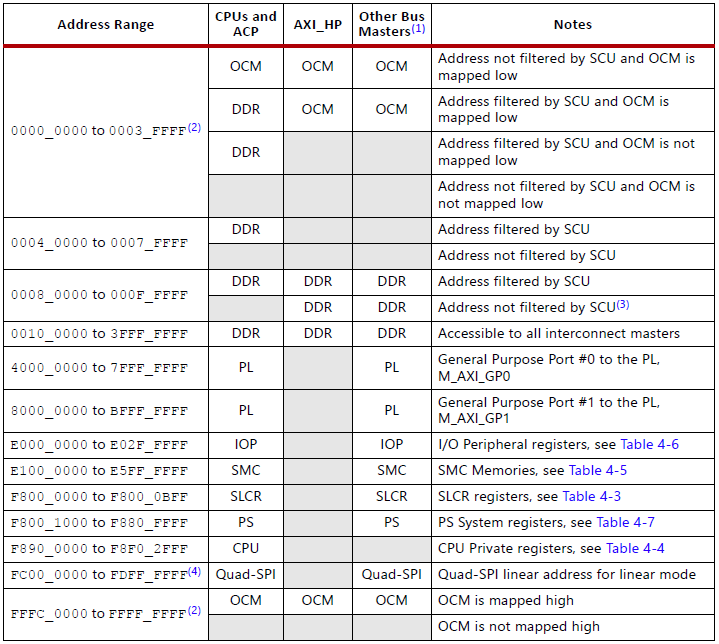
\includegraphics[width=10cm,height=\textheight,keepaspectratio]{images/AddressMapZynq.png}
	\caption[]{Address Map des Zynq}
	\label{fig:AddressMapZynq}
\end{figure}





	\chapter{OpenOCD}
% TODO: referenz openocd doku
% \ref{bib:OpenOCDDoku}
% TODO: CLI beschreiben / putty
% OpenOCD ist ein ''On-Chip Debugger''.\cite{bib:OpenOCDHome}
% Diese Bezeichnung ist allerdings etwas irreführend.
% TODO: Debugger früher erklären (Urs)
% TODO: FT2232 erklären (Urs)
OpenOCD\footnote{http://openocd.org/about/} bildet den Software-Teil eines Debuggers.
Zusammen mit einem Hardware-Adapter bildet OpenOCD einen vollständigen Debugger und kann als Ersatz für einen teuren Debugger, wie beispielsweise dem BDI3000 von Abatron, verwendet werden.

Der Adapter bildet dabei das elektrische Interface zum Prozessor und muss auch auf den Prozessor abgestimmt sein.
Relevant sind dabei unter anderem der Transport Layer (JTAG/SWD), das elektrische Potential und natürlich auch der physikalische Stecker.
In vielen Fällen basieren solche Adapter, wenn sie zusammen mit OpenOCD verwendet werden, auf dem FT2232-Chip von FTDI.
Solch ein generischer Adapter ist in der Abbildung \ref{fig:GenerischerFT2232Adapter} zu sehen.

\begin{figure}[htbp]
	\centering
		% 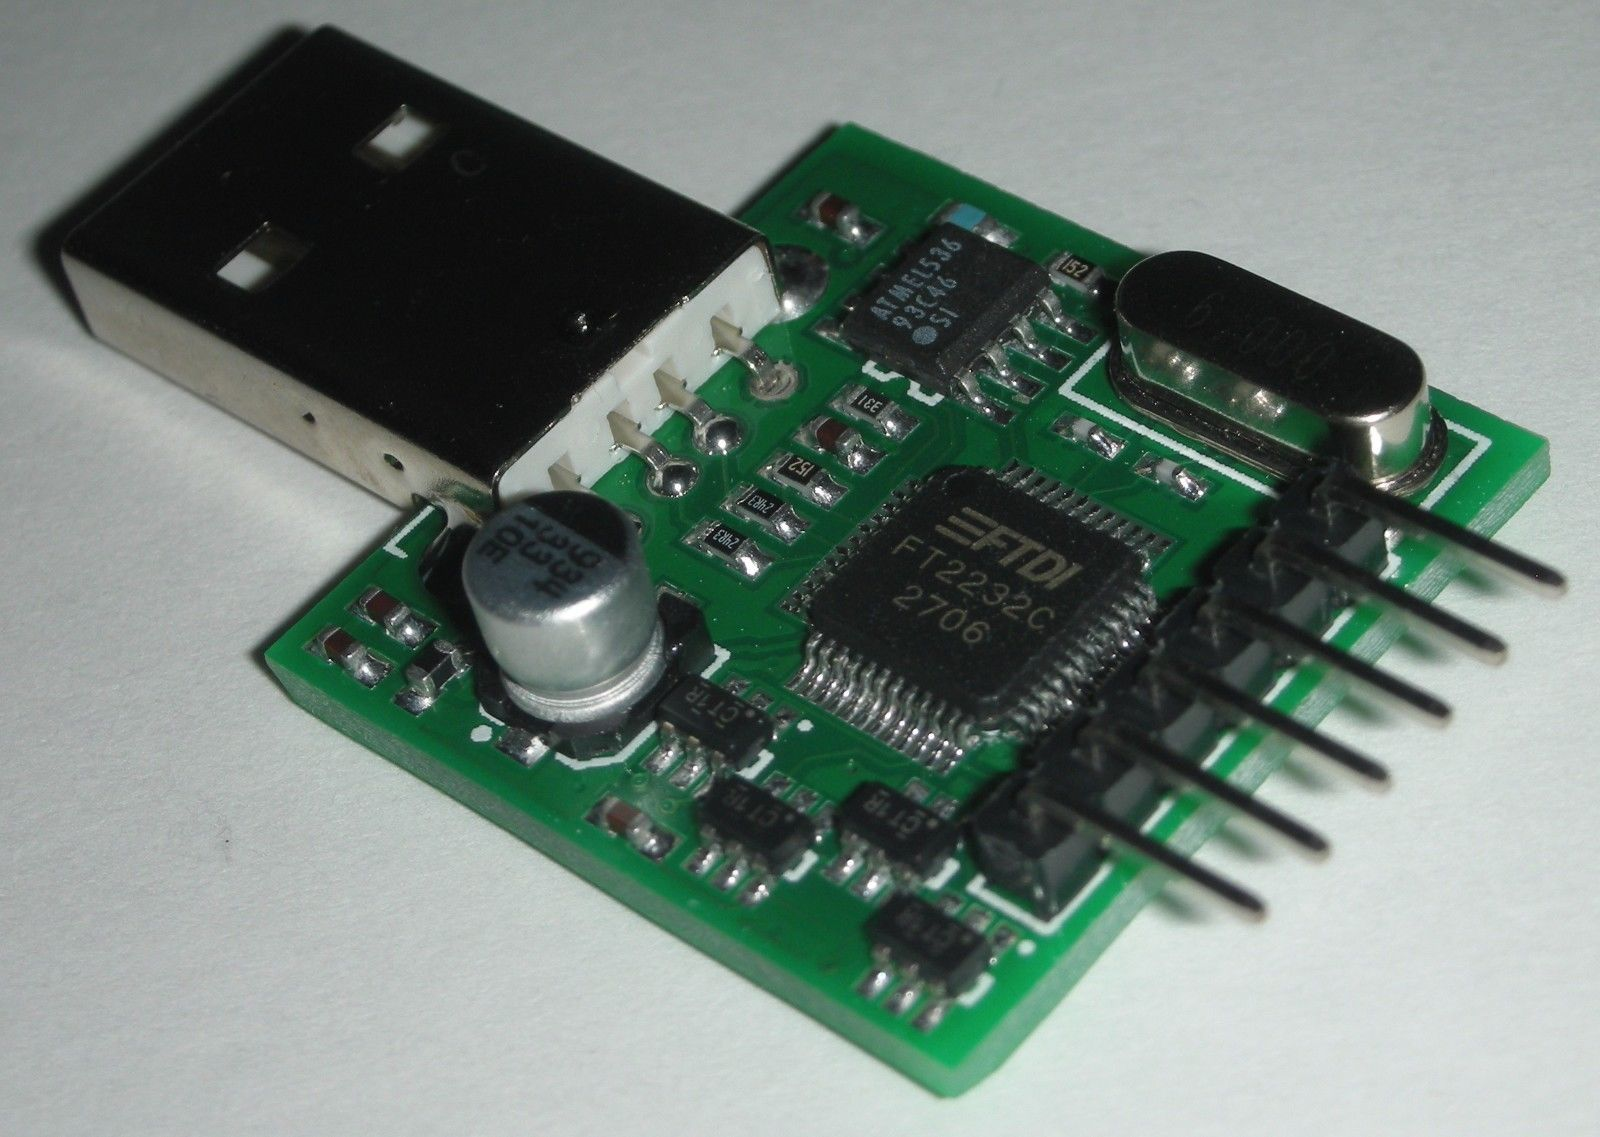
\includegraphics[width=\textwidth,height=\textheight,keepaspectratio]{images/JTAGAdapter.jpg}
		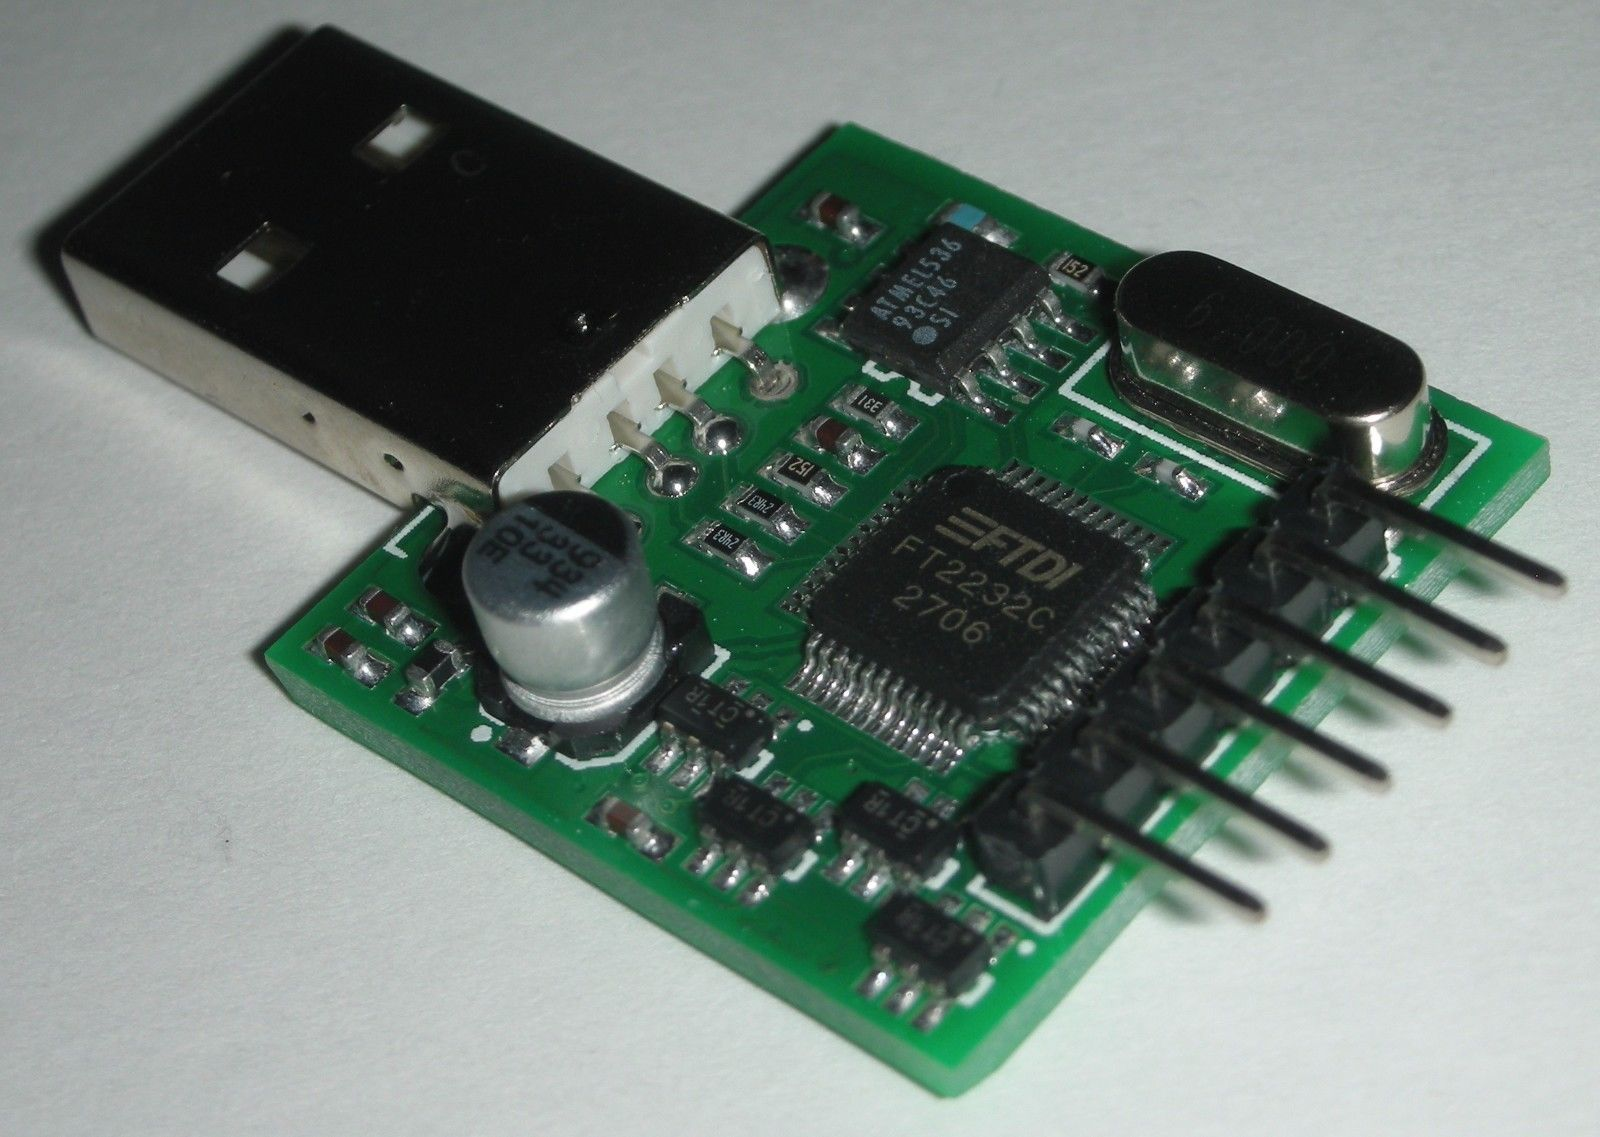
\includegraphics[width=7cm,keepaspectratio]{images/JTAGAdapter.jpg}
	\caption[Generischer JTAG Adapter mit einem FTDI FT2232]{Generischer JTAG Adapter mit einem FTDI FT2232\footnotemark}
	\label{fig:GenerischerFT2232Adapter}
\end{figure}
\footnotetext{https://www.ebay.com/itm/FPU1-FTDI-FT2232-USB-JTAG-XILINX-FPGA-CPLD-programmer-cable-/181635528314 Seite 5}

Bei Experimentierboards ist der FT2232 oft auch direkt auf das Board aufgelötet.
So kann eine einfache USB-Verbindung genutzt werden, um den Prozessor zu debuggen.
Beim Zybo wurde ebenfalls dieser Ansatz verfolgt.
Aus diesem Grund reicht ein einfaches USB Kabel um den Prozessor des Zybos auf einer Hardwareebene debuggen zu können.



\section{Softwareinstallation der OpenOCD-Toolchain}
\label{kapitel:SoftwareinstallationOpenOCDToolchain}
Um OpenOCD nutzen zu können, muss auch der richtige USB-Treiber installiert sein.
In den folgenden Kapiteln wird erklärt, wie der Treiber und auch OpenOCD-Software installiert werden kann.


\subsection{Softwareinstallation - OpenOCD}
OpenOCD kann direkt aus dem Sourcecode kompiliert werden\footnote{http://sourceforge.net/p/openocd/code/} oder es können vorkompilierte Binaries verwendet werden.
Für diese Arbeit wurde das vorkompilierte Windows Binaries\footnote{http://www.freddiechopin.info/en/download/category/4-openocd?download=154\%3Aopenocd-0.10.0} für ARM-Cores mit der Version 0.10.0 verwendet.

Das eigentliche Binary befindet sich im Ordner:\\
\texttt{/openocd-0.10.0/bin-x64/} 

Das Open OCD User Manual\cite{bib:OpenOCDDoku} befindet sich im Ordner:\\
\texttt{/openocd-0.10.0/} 


\subsection{Softwareinstallation - USB-Driver WinUSB}
\label{kapitel:usbTreiber}
Damit OpenOCD mit dem FT2232-Chip kommunizieren kann, werden die richtigen USB-Treiber benötigt.
Die Installation der Treiber ist am einfachsten mit dem \textit{USB Driver Tool}\footnote{http://visualgdb.com/UsbDriverTool/}.

Das Zybo muss per USB mit dem PC verbunden sein, damit der Treiber installiert werden kann.
Wenn der Jumper '\textit{J15}' auf USB gesetzt ist, wird keine zusätzliche Stromversorgung für das Zybo benötigt.

Wird das \textit{USB Driver Tool} geöffnet, dann werden alle USB Devices aufgelistet.
Das Device mit der \textit{Vendor ID=0403}, der \textit{Device ID=6010} und dem \textit{Interface 0} ist das JTAG Interface des FT2232.
Mit einem Rechtsklick kann \textit{Install WinUSB} ausgewählt und der Treiber installiert werden.
Abbildung \ref{fig:InstallWinUSBDriver} zeigt die Liste mit allen USB Devices und das Kontextmenü für die Installation des richtigen Treibers.
Um den Standardtreiber wieder zu installieren, kann einfach \textit{''Restore default driver''} ausgewählt werden.
Nachdem das Zybo einmal aus- und wieder einschaltet wird, ist der Treiber einsatzbereit.

Das Device mit der \textit{Vendor ID=0403, Device ID=6010} und \textit{Interface \textbf{1}} ist die UART-Verbindung zum Prozessor.
Dieser Treiber darf \textbf{nicht} ersetzt werden.

\begin{figure}[htbp]
	\centering
		% 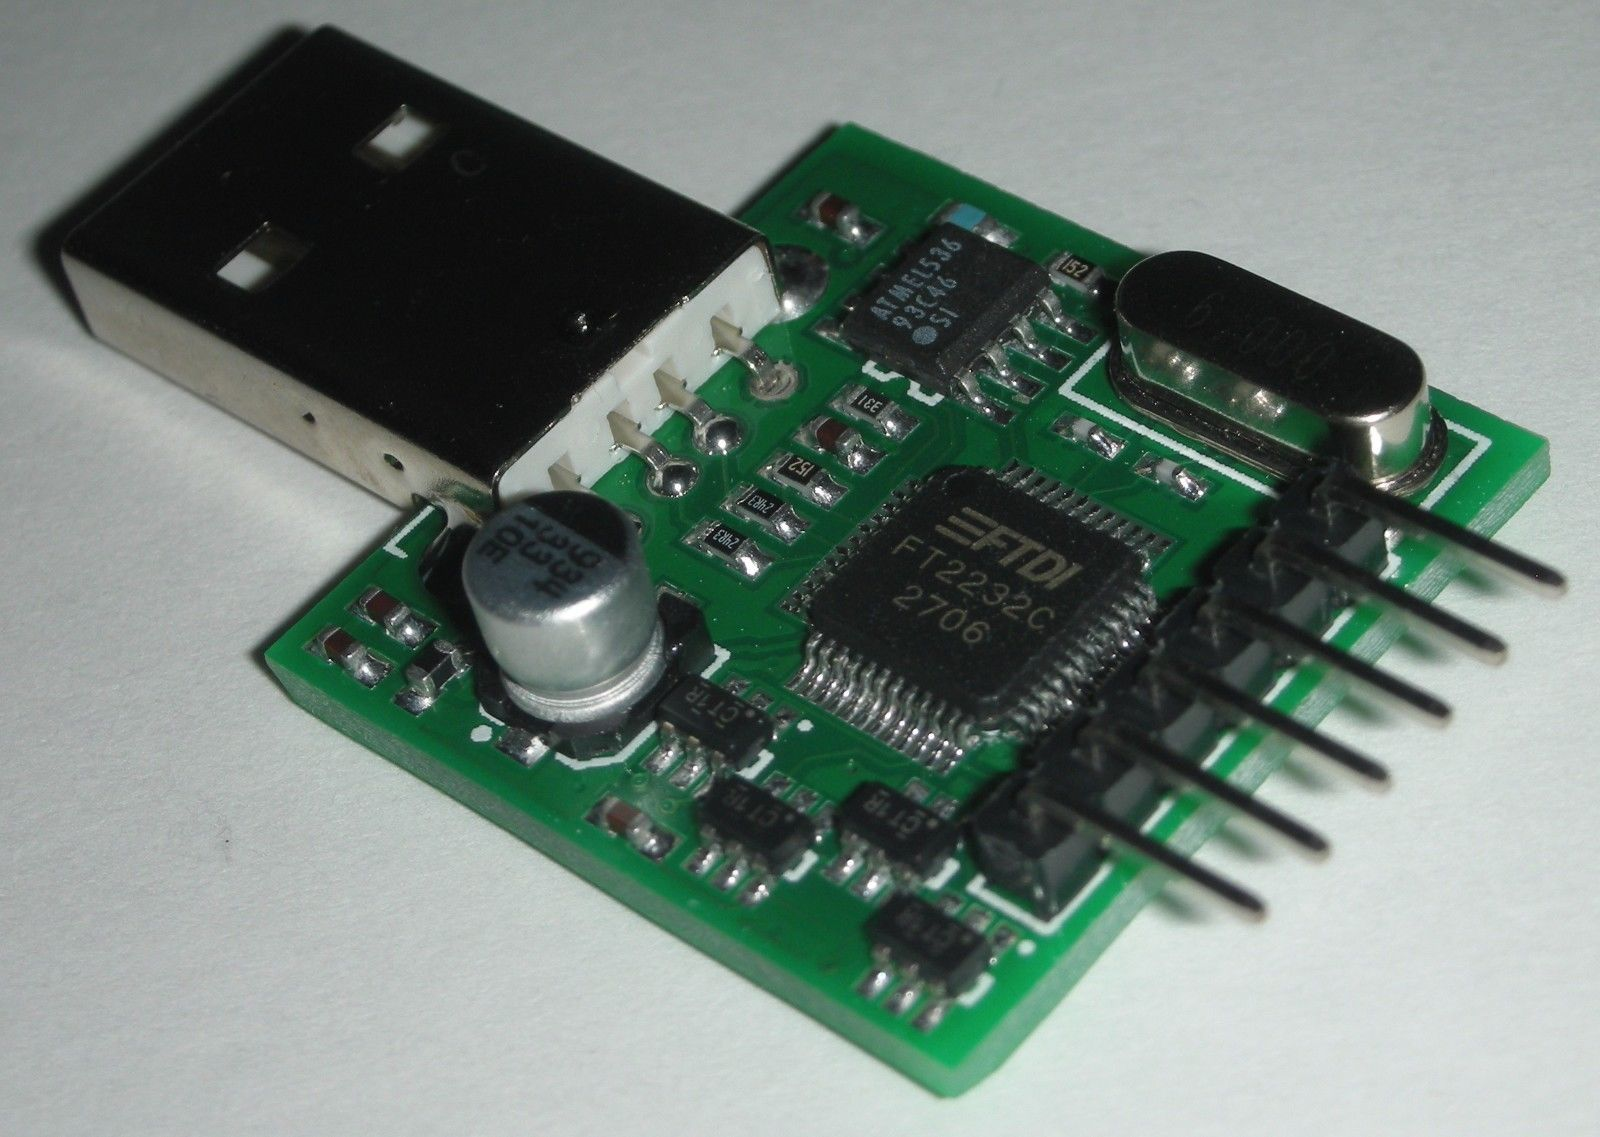
\includegraphics[width=\textwidth,height=\textheight,keepaspectratio]{images/JTAGAdapter.jpg}
		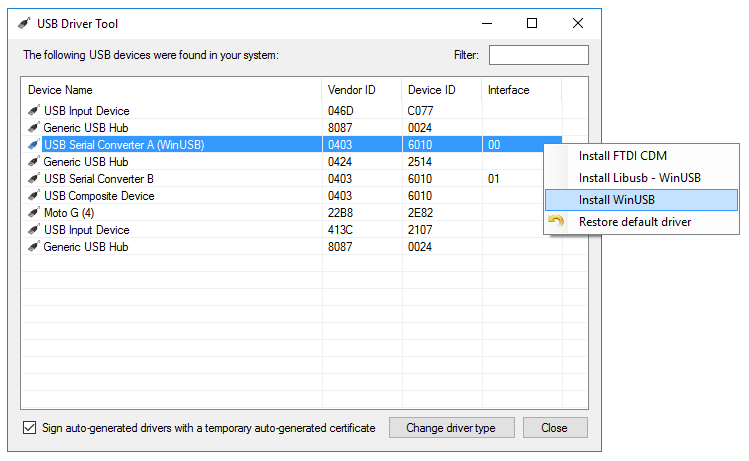
\includegraphics[width=12cm,keepaspectratio]{images/InstallWinUSBDriver.png}
	\caption{Installation des \textit{WinUSB} Treibers mit dem \textit{USB Driver Tool}}
	\label{fig:InstallWinUSBDriver}
\end{figure}


\section{OpenOCD CLI - Command Line Interface}
Das CLI (\textit{Command Line Interface}) ist eine einfache Methode um mit dem Debugger zu kommunizieren.
Sobald OpenOCD gestartet wurde, kann über den Port 4444, z.B. mit \textit{Putty}, auf dem \textit{Localhost} eine Telnet-Verbindung aufgebaut werden.
Der Befehl \texttt{''help''} listet alle zulässigen Befehle auf.

In den folgenden Kapiteln wird folgende Notation verwendet, um einen CLI-Befehl zu beschreiben:\\
(\texttt{CLI: Befehl})


\section{OpenOCD Konfiguration}
% TODO: zum starten siehe kapitel ...
% TODO: Files anhängen
% nicht einfach
% spezielle sprache jim-tcl
OpenOCD unterstützt eine Vielzahl von Adaptern und Targets (Prozessoren).
Beim Start muss die Software für die verwendete Hardware konfiguriert werden.
Die Konfiguration erfolgt mit Konfigurationsscripts (*.cfg) in der Scriptsprache \textit{Jim-Tcl}\footnote{http://jim.tcl.tk/index.html/doc/www/www/index.html}.
\textit{Jim-Tcl} ist eine abgespeckte Version von \textit{Tcl}\footnote{http://www.tcl.tk}.

Normalerweise werden die Scripts in die drei Gruppen \textit{interface, board} und \textit{target} aufgeteilt.
So kann einfach ein Script ausgewechselt werden, wenn man den gleichen Adapter aber einen anderen Prozessor verwenden will.
Im Pfad \texttt{openocd-0.10.0/scripts} befindet sich eine Sammlung von Konfigurationsscripts für Standardhardware.

Mit folgendem Befehl kann OpenOCD mit der passenden Konfiguration für das Zybo gestartet werden:\\
\texttt{openocd -f zybo-ftdi.cfg -f zybo.cfg}


\subsection{OpenOCD Konfiguration - Interface}
Die Interfacekonfiguration beschreibt hauptsächlich den verwendeten Adapter.
Da beim Zybo kein Adapter verwendet wird, sondern der aufgelötete FT2232, wird mit diesem Script der FTDI-Chip und dessen Anbindung an den Zynq konfiguriert.

Da ein FTDI-Chip als Interface verwendet wird, sollte ein passender Script unter \textit{openocd-0.10.0/scripts/ interface/ftdi/} zu finden sein.
Keiner der Scripts passt vom Namen her auf \textit{Zybo} oder \textit{FT2232}.
Eine Google Suche nach einem passenden Script war erfolgreicher.
Ein Github User mit dem Namen \textit{emard} hat folgenden Script in einem von seinen Repositories\footnote{https://github.com/f32c/f32c/blob/master/rtl/proj/xilinx/zybo/xram\_bram\_hdmi\_ise/zybo.ocd} gespeichert:

\textit{zybo-ftdi.ocd:}
\lstset{language=tcl}
\begin{lstlisting}[frame=single]
#
# ZYBO ft2232hq usbserial jtag
#

interface ftdi
ftdi_device_desc "Digilent Adept USB Device"
ftdi_vid_pid 0x0403 0x6010

ftdi_layout_init 0x3088 0x1f8b
#ftdi_layout_signal nTRST -data 0x1000 -oe 0x1000
# 0x2000 is reset
ftdi_layout_signal nSRST -data 0x3000 -oe 0x1000
# green MIO7 LED
ftdi_layout_signal LED -data 0x0010
#ftdi_layout_signal LED -data 0x1000

reset_config srst_pulls_trst

\end{lstlisting}

Zeile 5 bis 7 konfigurieren das Interface als ein Standard-FTDI-Interface.
Von OpenOCD werden neben dem FT2232 auch noch andere Chips unterstützt.
Zeile 7 definiert die \textit{Vendor} und \textit{Device-ID} des USB Devices.


\subsubsection{Resetverhalten}
Liest man aus einer unerlaubten Speicheradresse (\texttt{CLI: mdw 0x40000000}), dann hängt sich die Debug-Peripherie des Zynq auf.
Nach einem unerlaubten Speicherzugriff können auch keine erlaubten Speicherstellen mehr gelesen werden.
Beim Versuch erscheint die Fehlermeldung:\\
\texttt{Timeout waiting for cortex\_a\_exec\_optcode}.\\
Wahrscheinlich ist die \textit{CoreSight} Debug-Peripherie abgestürzt oder in einem undefinierten Zustand.
Aus diesem Grund bekommt OpenOCD keine Antwort vom Zynq, wenn versucht wird, eine Speicheradresse zu lesen.
Mit einem manuellen Powercycle des Zybos kann die Hardware wieder zurückgesetzt werden.

Im Supportbereich der Xilinx Homepage\footnote{https://www.xilinx.com/support/answers/63871.html} ist eine mögliche Erklärung für dieses Verhalten zu finden.
In diesem Artikel wird beschrieben, dass die Fehlermeldung ''\textit{Invalid address - it can hang PS interconnect}'' erscheint, wenn mit dem XSDB (\textit{Xilinx System Debugger}) auf bestimmte Adressbereiche zugegriffen wird.
Die Vermutung liegt nahe, dass der XSDB merkt, wenn auf eine \textit{''Invalid address''} zugegriffen werden soll.
Dieser Befehl wird abgefangen und stattdessen wird die Fehlermeldung angezeigt, so dass der \textit{''PS interconnect''}, also der Bus innerhalb des Zynq, nicht abstürzen kann.
OpenOCD fängt einen solchen invaliden Zugriff nicht ab, was dann zum Absturz des \textit{''PS interconnect''} führt.
Da auch die Peripherie für den Debugger im Zynq von diesem \textit{Interconnect} abhängig ist, stürzt auch die Debug-Peripherie ab, sobald auf einen ungültigen Adressbereich zugegriffen wird.

Mit OpenOCD ist es grundsätzlich möglich, einen Reset automatisch durchzuführen.
Dabei wird zwischen einem SRST (\textit{System Reset}) und dem TRST (\textit{TAP Reset}) unterschieden.
% Dabei wird zwischen einen SRST (\textit{System Reset}) und dem \textit{TAP\footnote{Test Access Port} Reset} (TRST) unterschieden.
Der SRST führt einen Powercycle vom ganzen System durch, der TRST setzt mit einem JTAG-Befehl nur den TAP (\textit{Test Access Port}) zurück.

% TODO: warum memory location nicht erlaubt
Beim obigen Script ist aber das Resetverhalten nicht sauber definiert.
Mit dem Befehl \texttt{''CLI: reset halt''} sollte der FT2232 einen Reset des ganzen Zynq durchführen.
Der Befehl führt aber zur Fehlermeldung:\\
\texttt{
% ...\\
zynq.cpu0: how to reset?\\
% ...
}

Im OpenOCD User Manual\cite{bib:OpenOCDDoku} in \textit{''Kapitel 9: Reset Configuration''} ist beschrieben, wie das Resetverhalten konfiguriert werden kann.
Mit dem Script-Befehl \texttt{''reset\_config srst\_only''} wird der TAP Reset ignoriert.
Da jetzt nur noch der SRST und nicht mehr der TRST verwendet wird, kann das Problem auf den SRST begrenzt werden.

Wenn OpenOCD mit der neuen Konfiguration neu gestartet wird, scheint der Befehl \texttt{''CLI: reset halt''} zu funktionieren.
Wird vorher aber wieder auf eine ungültige Speicherstelle zugegriffen, dann erscheint beim Reset die Fehlermeldung:\\
\texttt{
% ...\\
Timeout waiting for dpm prepare\\
% ...\\
}\\
Das erneute Timeout legt die Vermutung nahe, dass der Zynq nicht ordentlich zurückgesetzt wurde.

Zeile 12 \texttt{''ftdi\_layout\_signal nSRST -data 0x3000 -oe 0x1000''} konfiguriert die I/O Pins des FT2232, welche für den System Reset verwendet werden.
Im elektrischen Schema des Zybos (siehe Anhang \ref{anhang:schemaZybo}) könnte man überprüfen, welche I/Os des FT2232 tatsächlich für den Reset verwendet werden.
Die Seite mit dem Schema für den FT2232, Seite 7, ist aber als einzige Seite im Schema nicht veröffentlicht worden.
Die korrekten I/O Pins lassen sich also nicht mit dem Schema ermitteln.
Direkt aus dem PCB sind die Verbindungen auch nicht eindeutig ablesbar, da es sich beim Zybo um ein relativ dichtes PCD mit mehreren Lagen handelt.

Im OpenOCD User Manual\cite{bib:OpenOCDDoku} wird der \texttt{''ftdi\_layout\_signal nSRST} genauer beschrieben.
Der Switch \textit{-data 0x3000} definiert alle relevanten Pins für den SRST und \textit{-oe 0x1000} konfiguriert alle Ausgänge.
In einem Versuch wurden diverse Kombinationen für die beiden Switches ausprobiert.
Keine Kombination mit nur einem Pin (z.B. \textit{-data 0x2000} mit \textit{-oe 0x2000}) hat funktioniert.
Es hat sich dann aber herausgestellt, dass die Kombination \textit{-data 0x3000} mit \textit{-oe 0x3000} tatsächlich einen System Reset ermöglicht.

Weil der Debugger direkt nach dem SRST versucht mit dem Zynq zu kommunizieren, tritt folgende Fehlermeldung auf:\\
\texttt{
...\\
Invalid ACK (7) in DAP response\\
JTAG-DP STICKY ERROR\\
...\\
}
Mit dem Kommando \texttt{''adapter\_nsrst\_delay 40''} wartet der Debugger nach dem SRST zusätzliche 40 Millisekunden.
Diese Wartezeit genügt, damit die FTDI-Interface des Zynq wieder betriebsbereit ist, wenn der Debugger versucht zu kommunizieren.



\subsection{OpenOCD Konfiguration - Board}
Da beim Zybo der Adapter direkt auf dem Board ist, ist die Bordkonfiguration bereits im Konfigurationsscript für das Interface enthalten.

\subsection{OpenOCD Konfiguration - Target}
Für das Target, in diesem Fall der Zynq 7000 SOC, ist bereits ein Script unter \textit{openocd-0.10.0/scripts/ target/zynq\_7000.cfg} enthalten.
In diesem Script werden nicht nur beide Kerne des Prozessors definiert, sondern auch ein TAP für das FPGA.
Es ist also auch möglich, den FPGA mit dieser Toolchain zu laden.
% zynq_7000.cfg


\section{CLI-OpenOCD-Toolchain}
\label{section:CLI-OpenOCD-Toolchain}
Die \textit{CLI-OpenOCD-Toolchain} ist ein Eclipse-Plugin, welches in Kombination mit \textit{deep} verwendet werden kann.
Es erfüllt die gleichen Funktionen wie die bestehende \textit{Abatron-Toolchain}.

Das Plugin kann von folgendem Repositorie geklont werden:
% TODO0: repo anlegen
% \texttt{}


	\chapter{ELF Dateiformat}
ELF (\textit{Executable and Linking Format}) ist das Standard-Binärformat von vielen UNIX-ähnlichen Betriebssystemen.
Es wird für ausführbare Dateien und auch für Libraries verwendet.
Es können auch notwendige Informationen für den Debugger in dieses Format gepackt werden.
In diesem Kapitel wird der grundlegende Aufbau des Formates erklärt.
Zusätzlich wird auf einige Details genauer eingegangen, die für einen Debugger relevant sind.

Einen sehr guten Einstieg bietet auch der Artikel \textit{''Understanding the ELF''}\footnote{\ \ Direkter Link: \ \ \ \ \ \ \ \ \ https://medium.com/@MrJamesFisher/understanding-the-elf-4bd60daac571\\ Archivierter Link: https://web.archive.org/web/20180705122234/https://medium.com/@MrJamesFisher/understanding-the-elf-4bd60daac571} von James Fisher.
In der Spezifikation für das ELF Format\cite{bib:ELFSpecification} ist der Aufbau des Formates im Detail erklärt.


\section{Nützliche Tools}
\textit{readelf} ist ein nützliches Linux-Tool um Informationen einer ELF-Datei anzeigen zu lassen.
Unter Windows kann diese Software ebenfalls in der Shell verwendet werden, wenn \textit{mingw}\footnote{http://www.mingw.org/} installiert ist.
% mingw

\section{Grundlegender Aufbau}
\begin{figure}[htbp]
	\centering
		% 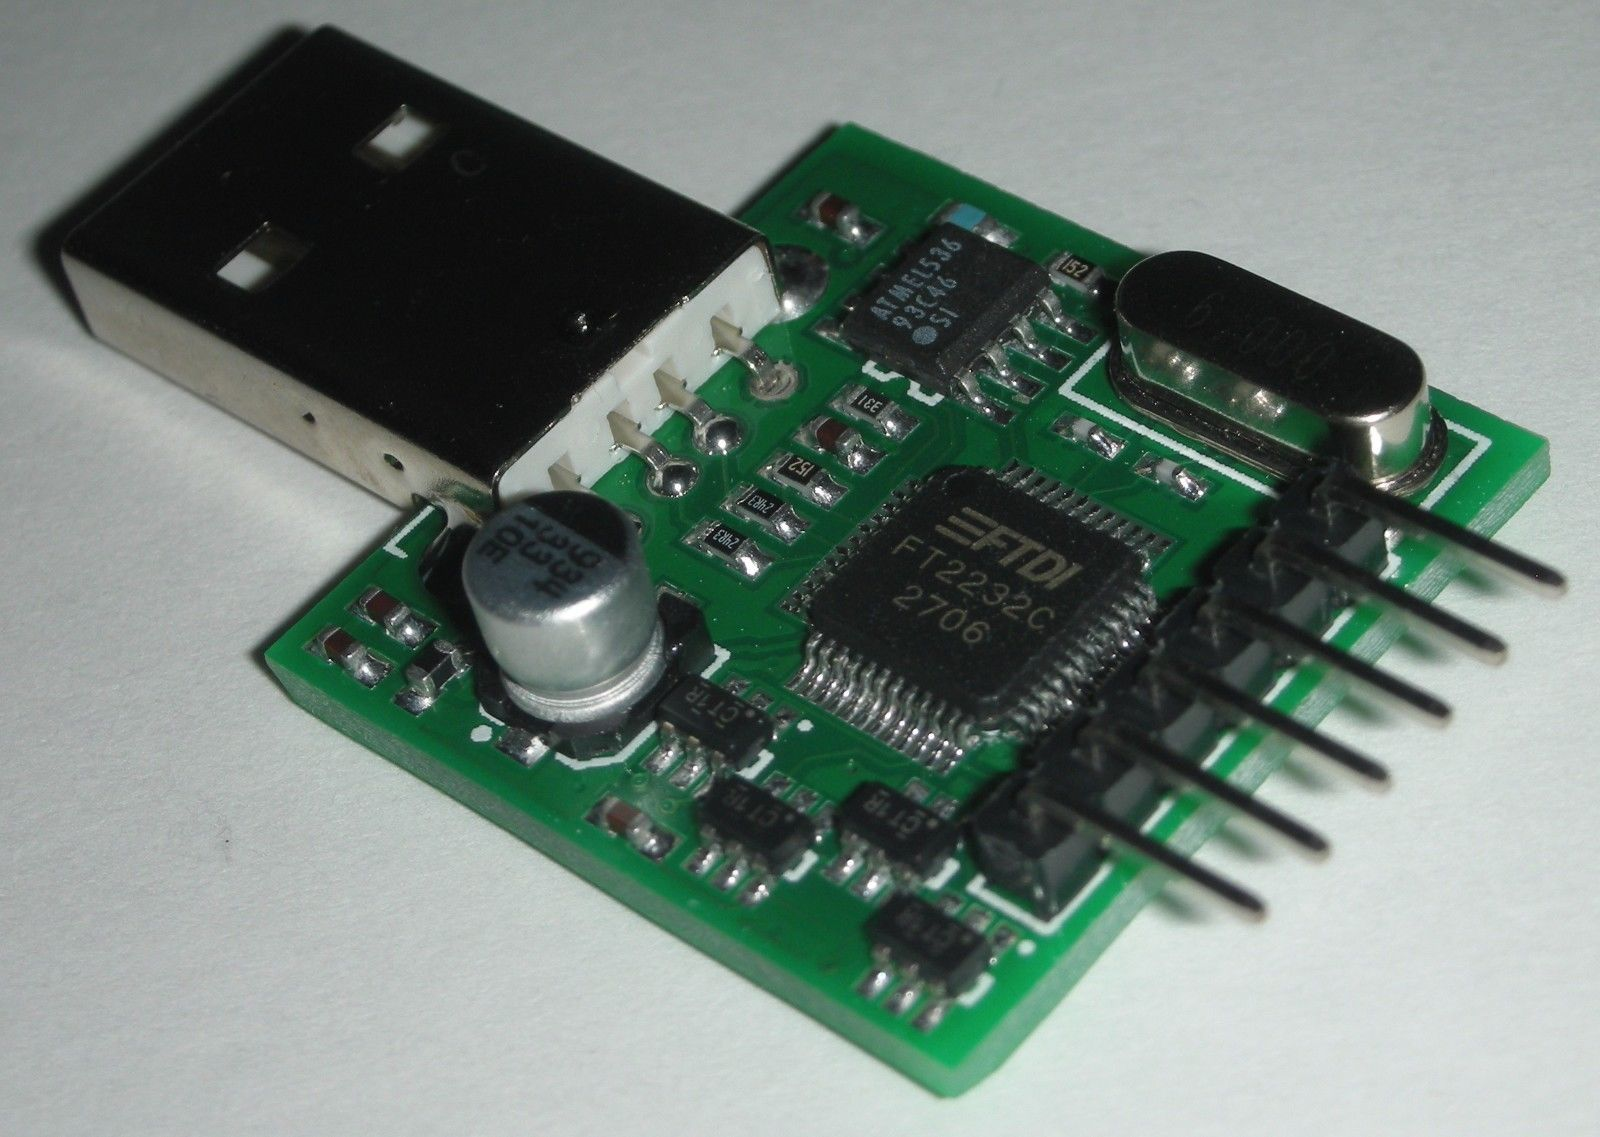
\includegraphics[width=\textwidth,height=\textheight,keepaspectratio]{images/JTAGAdapter.jpg}
		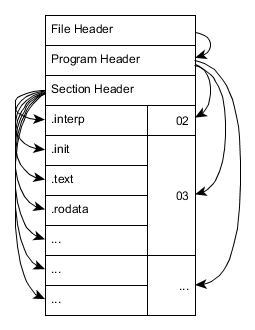
\includegraphics[width=7cm,keepaspectratio]{graphs/elf.png}
	\caption[Der Aufbau von einer ELF Datei]{Der Aufbau von einer ELF Datei\footnotemark}
	\label{fig:ELFStructure}
\end{figure}
\footnotetext{https://slideplayer.com/slide/6444592/}

% Auf Wikipedia\footnote{https://en.wikipedia.org/wiki/Executable\_and\_Linkable\_Format} ist der Aufbau sehr gut beschrieben.


% \begin{figure}[htbp]
% 	\centering
% 		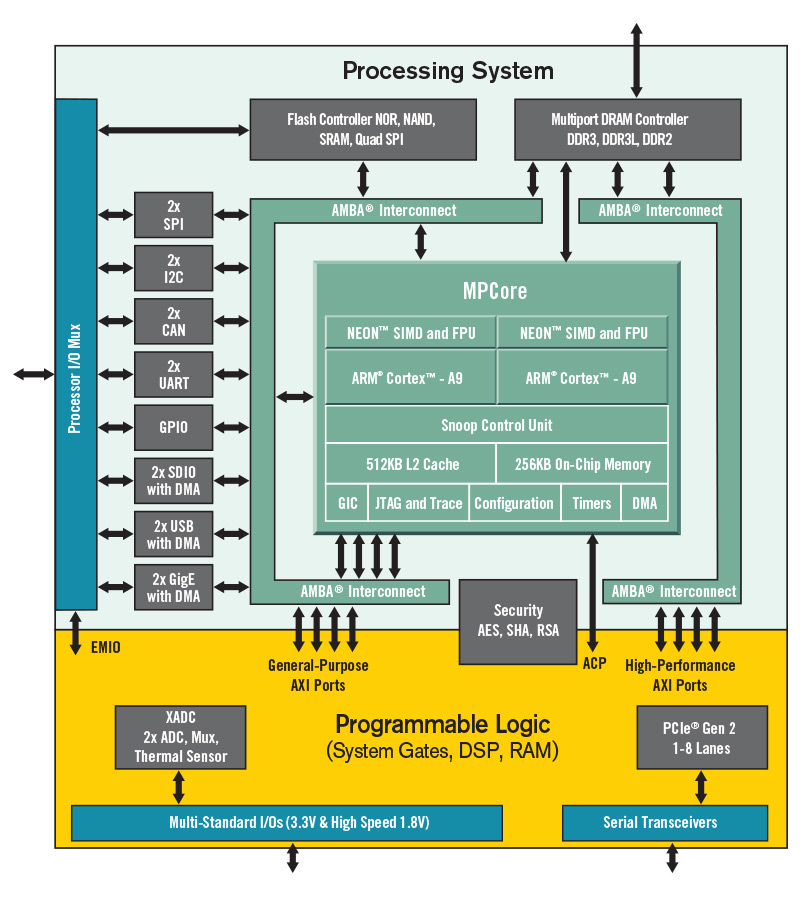
\includegraphics[width=10cm,height=\textheight,keepaspectratio]{images/zynqBlockDiagram.png}
% 	\caption[Block Diagramm Zynq\-7000]{Block Diagramm Zynq\-7000\footnotemark}
% 	\label{fig:BlockDiagrammZynq}
% \end{figure}
% \footnotetext{https://www.xilinx.com/products/silicon-devices/soc/zynq-7000.html}

Der \textit{File Header} beinhaltet Metainformationen über die Datei selbst.
Mit \texttt{''readelf filename -Wh''} lässt sich der \textit{File Header} einer Datei anzeigen.

Der \textit{Program Header} kann mit \texttt{''readelf filename -Wl''} ausgegeben werden.
Darin ist enthalten, welchen Offset die einzelnen Segmente innerhalb der Datei haben.
Zusätzlich ist auch definiert, zu welcher Speicheraddresse (im RAM) die Segmente kopiert werden, wenn das Programm gestartet wird und was für Rechte (ausführbar, lesen und schreiben) jedes Speichersegment hat.
Wird, z.B. wegen eines nicht initialisierten Pointers, in einer Speicherstelle im Memory gelesen, die kein \textit{''read flag''} hat, wird ein \textit{Segmentation Fault} ausgelöst.
% TODO: welches segment wird beim gdb geschrieben?
Der \textit{gdb} nutzt Informationen aus diesem Header um zu bestimmen, welche binären Daten mit dem Befehl \texttt{''load''} an welchen Speicherort kopiert werden sollen.
Ein Segment beinhaltet ein oder mehrere \textit{Sections}.
% TODO: satz sollte klarer sein
% Die Segmente sind beim Ausführen der Datei relevant.

Im \textit{Section Header} sind alle \textit{Sections} beschrieben.
Mit \texttt{''readelf filename -WS''} kann man sehen, dass jede \textit{Section} unter anderem einen Namen, einen Typ, eine Adresse (absolut) und einen Offset (relativ, innerhalb der ELF-Datei) enthält.
Jede \textit{Section} beinhaltet einen anderen Teil des Programms.
Die folgende Liste gibt eine kleine, nicht vollständige Übersicht über die einzelnen \textit{Sections}:
\begin{itemize}
	\item \texttt{.text}\ \ \ \ \ \ \ \ \ Der ausführbare Teil des Programms.
	\item \texttt{.data}\ \ \ \ \ \ \ \ \ Enthält die globalen Variablen.
	\item \texttt{.rodata}\ \ \ \ \ Enthält alle Strings.
	\item \texttt{.stab}\ \ \ \ \ \ \ \ \ Enthält die STABS Debuginformationen. Mehr dazu im Kapitel \ref{label:stabs} 
	\item \texttt{.stabstr}\ \ \ Enthält die STABS Debuginformationen. Mehr dazu im Kapitel \ref{label:stabs} 
\end{itemize}
Der Compiler nutzt die \textit{Secitons} um das Programm in logische Einheiten zu unterteilen.
% Eine \textit{Seciton} ist eine Logische Einheit eines Programms, deren Einteilung besonders für den Compiler Vorteile bringt.


\subsection{Informationen für den Debugger}
Zusätzliche Informationen für den Debugger werden ebenfalls im ELF Format gespeichert.
Moderne Compiler verwenden hauptsächlich das DWARF-Format und nicht das veraltete STABS-Format.
Trotzdem wird von aktuellen Compilern und auch Debuggern das veraltete STABS-Format immer noch unterstützt.

DWARF ist flexibler und hat einen besseren funktionalen Umfang als das STABS-Format, aber die manuelle Implementation ist aufwändiger.





\section{STABS}
\label{label:stabs}
% TODO: Debugging-Informationen oder Debugginginformationen.
STABS ist ein Datenformat für Debug-Informationen.
Die Informationen sind als Strings in \textit{\textbf{S}ymbol \textbf{TA}ble \textbf{S}trings} gespeichert.
% Obwohl dieses Format veraltet ist, wird dieses Format in dieser Arbeit verwendet, weil es am einfachsten manuell zu implementieren ist.
% Bei moderneren Systemen wurde das STABS Format durch das neuere DWARF-Format abgelöst.

\subsection{Zielsetzung}
Es soll getestet werden, ob es möglich ist, eine \textit{deep}-Applikation mit dem \textit{gdb} zu debuggen.
Dazu benötigt der \textit{gdb} neben dem ausführbaren Maschinencode zusätzliche Debug-Informationen in der Form von STABS oder im DWARF-Format.
In beiden Fällen werden die Informationen im ELF-Format eingebettet.

In dieser Arbeit wird ein Demo-Programm mit STABS implementiert, da STABS-Informationen einfacher manuell zu implementieren sind als DWARF-Informationen.


\subsection{Aufbau des STABS Formats}
Eine einheitliche Dokumentation für STABS gibt es nicht.
Es ist nicht einmal sicher bekannt, wer der ursprüngliche Erfinder von dieses Formats ist.
In der Dokumentation von \textit{Sourceware}\footnote{\ \ Direkter Link: \ \ \ \ \ \ \ \ \ https://www.sourceware.org/gdb/onlinedocs/stabs.html\\ Archivierter Link: \ \ \ https://web.archive.org/web/20180717131349/https://www.sourceware.org/gdb/onlinedocs/stabs.html} wird aber Peter Kessler als Erfinder genannt.

Der Aufbau dieses Formats wird in der oben genannten Dokumentation von \textit{Sourceware} und in der Dokumentation von der \textit{''University of Utha''}\footnote{\ \ Direkter Link: \ \ \ \ \ \ \ \ \ http://www.math.utah.edu/docs/info/stabs\_toc.html\\ Archivierter Link: \ \ \ https://web.archive.org/web/20180717132825/http://www.math.utah.edu/docs/info/stabs\_toc.html} beschrieben.
Obwohl diese Dokumentationen zum Teil sehr detailliert sind, sind sie nicht lückenlos.
Im Folgenden wird nur auf die Grundlagen eingegangen, die für das Beispielprogramm relevant sind.

STABS-Informationen sind in einzelne Informations-Elemente, so genannte \textit{directives}, unterteilt.
Jede Direktive ist entweder ein \textit{''.stabs''} (String), ein \textit{''.stabn''} (Integer) oder ein \textit{''.stabd''} (Dot).
Zusätzlich hat jede Direktive einen bestimmten Typ.
Der Typ definiert, was die einzelnen Direktiven genau beschreiben.
Um die Leserlichkeit zu verbessern sind alle Typen in der Datei \textit{''stabs.include''} (Siehe Anhang \ref{anhang:stabs.include}) definiert.
Im Kapitel 12 der Dokumentation der \textit{''University of Utha''} sind die einzelnen Typen genau beschreiben.
% TODO grafische übersicht stabs-stabstring-typ

Die STABS werden mit folgender Syntax im Assembler-Code definiert:\\
\lstset{language=plain}
\begin{lstlisting}
.stabs ''string'',type,other,desc,value
.stabn type,other,desc,value
.stabd type,other,desc
\end{lstlisting}



\subsection{DWARF}
% TODO: DWARF erklären


\section{Demoprogramm mit STABS}
% TODO alle files im Anhang
In diesem Kapitel wird beschrieben wie ein Demoprogramm mit STABS-Informationen erstellt werden kann.
Das Demoprogramm soll dann mit dem \textit{gdb} direkt auf den Zynq geladen werden.
Zusätzlich sollen folgende \textit{gdb}-Features getestet werden:\\
\begin{enumerate}
	\item \textbf{Breakpoint}: Das Programm stoppt bei einer gewünschten Zeile im Java-Sourcecode.
	\item \textbf{Source lookup}: Wenn das Programm gestoppt wird, kann die entsprechende Zeile im Java-Sourcecode angezeigt werden.
	\item \textbf{Single-Stepping}: Nur eine Zeile im Java-Sourcecode ausführen und dann pausieren.
	\item \textbf{Variable auslesen}: Eine Java-Variable, z.B. ein Integer, auslesen.
	\item \textbf{Variable manipulieren}: Eine Java-Variable verändern.
	\item \textbf{Prozessor-Register auslesen}: Ein Register der CPU auslesen.
\end{enumerate}

\subsection{Vorgehen}
Um ein Demoprogramm zu erstellen, werden untenstehende Schritte durchgeführt.
Alle Schritte werden weiter unten im Detail erklärt.
Das Programm \textit{''loop''} soll für den \textit{gdb}-Test verwendet werden.
\textit{''loopExample''} ist ein Hilfsprogramm, das vom \textit{gdb} automatische generierte STABS enthält.
Es dient als Vorlage, um die richtigen STABS im Programm \textit{''loop''} hinzufügen zu können.

% Das Demoprogramm 
\begin{enumerate}
	\item \textbf{loop.java}: Demoprogramm als Java-Code Schreiben.
	% deep: java -> maschine
	\item Beispiel-Programm mit automatisch generierten STABS erstellen:
	\begin{enumerate}
		\item \textbf{loopExample.c}: Das Java-Programm manuell in C-Code übersetzen.
		\item \textbf{loopExample.o}: Das Programm mit STABS-Informationen kompilieren.
		\item \textbf{loopExample.Sd}: Das disassembliert Programm, um die STABS in einer leserlichen Form zu erhalten.
		\item \textbf{loopExample.host.c}: Leicht abgeändertes \textit{''loopExample.c''}, um ein ausführbares Programm für den Host-PC zu erhalten.
		\item \textbf{loopExample.host.a}: Ausführbares Programm für den Host-PC.
	\end{enumerate}
	\item Lauffähiges Programm für den Zynq mit manuell ergänzten STABS erstellen:
	\begin{enumerate}
		\item \textbf{Reset.Java}: Den Source-Code des Java-Programms in die Reset-Methode des \textit{deep}-Kernel kopieren.
		\item Den modifizierten Kernel mit \textit{deep} übersetzen.
		\item \textbf{loopMachineCode.txt}: Enthält den Maschinen-Code aus der \textit{ClassTreeView} von \textit{deep}.
		\item \textbf{loop.S}: Der aus \textit{''loopMachineCode.txt''} abgeleitete Assembler-Code.
		\item \textbf{loopWithSTABS.S}: Der Assembler-Code inklusive den manuell ergänzten STABS.
		\item \textbf{loopWithSTABS.o}: Kompiliertes Objekt aus dem Assembler-Code.
		\item \textbf{loopWithSTABS}: Gelinktes Objekt aus dem kompilierten Objekt.
		\item \textbf{loopWithSTABS.Sd}: Das disassemblierte Programm, um die STABS in einer leserlichen Form zu erhalten.
	\end{enumerate}
\end{enumerate}



\subsection{Java Demoprogramm}
Das unten stehende Programm ist das Testprogramm, dass von \textit{deep} in Maschinen-Code übersetzt werden soll und anschliessend manuell mit STABS ergänzt werden soll.

\lstset{language=java}
\begin{lstlisting}
static void reset() {



	US.PUTGPR(SP, stackBase + stackSize - 4);	// set stack pointer
	
	int x00 = 0;
	int x01 = 1;
	int x02 = 2;
	
	x00++;
	x01++;
	x02++;
	
	int x100 = 100;
	for(int i=0; i<10; i++){
		x100 += 10;
   }
		
	x100++;
	x100++;
	x100++;
	x100++;
	x100++;

	US.ASM("b -8"); // stop here
}
\end{lstlisting}

In diesem Beispiel wird die \texttt{reset()}-Methode genutzt, da sie bei \textit{deep} als erstes beim Booten ausgeführt wird.
\texttt{''US.PUTGPR''} in Zeile 5 ist natürlich keine Java Methode.
Da Low-Level-Operationen, wie die Initialisierung des Stackpointers, mit Java normalerweise nicht möglich sind, wird hier die entsprechende \textit{deep}-Instruktion verwendet.


\subsection{Beispiel-Programm ''loopExample''}
Der Code in \textit{''loopExample.c''} im Anhang \ref{anhang:stabs} ist fast identisch mit dem Code des Java Demoprogramms.
Es wurden nur einige Änderungen gemacht, damit der Code als C-Programm kompiliert werden kann.
\texttt{c\_entry()} ist der Eintrittspunkt des Programms und erfüllt im embedded Bereich eine ähnliche Aufgabe wie die  \texttt{main()}-Methode in einem generischen C-Programm.

Mit dem PowerShell-Script \textit{''make\_loopExample.ps1''} im Anhang \ref{anhang:stabs} kann das C-Programm kompiliert werden.
Es erzeugt das Object-File \textit{''loopExample.o''} inklusive Debuginformationen im STABS Format.
Das disassemblierte Object-File wird als \textit{''loopExample.Sd''} gespeichert.
Im disassemblierten Object-File sind alle STABS-Informationen und auch der ausführbare Code als Assembler enthalten.
Der Assembler-Code und auch die STABS-Informationen können direkt \textit{''human readable''} gelesen werden, aber sie können nicht direkt in einem kompilierbaren Programm verwendet werden, da die Syntax nicht übereinstimmt.

Beispiel mit disassemblierter Syntax:
\lstset{language=plain}
\begin{lstlisting}
...
2      LSYM   0      0      00000000 44     int:t(0,1)=r(0,1);-2147483648;2147483647;
...
00000000 <c_entry>:
   0:	e92d0810 	push	{r4, fp}
\end{lstlisting}


Kompilierbare Assembler Syntax:
\lstset{language=plain}
\begin{lstlisting}
...
.stabs "int:t(0,1)=r(0,1);-2147483648;2147483647;",N_LSYM,0,0,0
...
c_entry:
push {r4, fp}
\end{lstlisting}


\subsection{Analyse der disassemblierten STABS}
\FloatBarrier

Die untenstehenden Direktiven sind ein Auszug aus der Datei \textit{''loopExample.Sd''} im Anhang \ref{anhang:stabs}.
Die Tabelle \ref{t-DisassemblierteSTABdirektive} beschreibt die Direktive 0 im Detail.
\lstset{language=plain}
\begin{lstlisting}
Symnum n_type n_othr n_desc n_value  n_strx String
...
0      SO     0      2      00000000 15     loopExample.c
1      OPT    0      0      00000000 29     gcc2_compiled.
2      LSYM   0      0      00000000 44     int:t(0,1)=r(0,1);-2147483648;2147483647;
...
51     GSYM   0      0      00000000 1919   global:G(0,1)
52     FUN    0      0      00000000 1933   c_entry:F(0,1)
53     SLINE  0      4      00000000 0 
54     SLINE  0      5      0000000c 0     
...
72     LSYM   0      0      fffffff0 1948   x00:(0,1)
73     LSYM   0      0      ffffffec 1958   x01:(0,1)
74     LSYM   0      0      ffffffe8 1968   x02:(0,1)
75     RSYM   0      0      00000004 1978   s:r(0,1)
76     LSYM   0      0      ffffffe4 1987   float0:(0,14)
77     LSYM   0      0      fffffff8 2001   int0:(0,1)
78     LBRAC  0      0      00000000 0      
79     LSYM   0      0      fffffff4 2012   i:(0,1)
80     LBRAC  0      0      00000060 0      
81     RBRAC  0      0      00000090 0      
82     RBRAC  0      0      000000c4 0      
83     SO     0      0      000000c4 0 
\end{lstlisting}

\begin{table}[H]
\caption{Disassemblierte STAB direktive}
\label{t-DisassemblierteSTABdirektive}
\begin{tabular}{|l|l|l|}
 \hline
\textit{Symnum}   & 0             & Eindeutige Identifikation der STAB-Direktive \\ \hline
\textit{n\_type}  & S0            & \begin{tabular}[c]{@{}l@{}}Typ der STAB-Direktive. Die SO-Direktive beschreibt das Source-File\\
									 welches die \texttt{''main()''}-Methode enthält. \end{tabular}                                       \\ \hline
\textit{n\_othr}  & 0             & Das \textit{other}-Feld wird normalerweise nicht genutzt und auf ''0'' gesetzt.                                         \\ \hline
\textit{n\_desc}  & 2             & \textit{''the starting text address of the compilation.''}\footnote{http://www.math.utah.edu/docs/info/stabs\_12.html\#SEC73}                                        \\ \hline
\textit{n\_value} & 00000000      & Dieser Integer wird hauptsächlich für \textit{.stabn}-Direktive genutzt.                                         \\ \hline
\textit{n\_strx}  & 15            & Start des Strings für die nächste Direktive                                         \\ \hline
\textit{String}   & loopExample.c & \begin{tabular}[c]{@{}l@{}}Der String, der die eigentliche Information enthält. In diesem Fall\\ 
									ist es das Source-File mit der \texttt{''main()''}-Methode.\end{tabular}            \\  \hline                           
\end{tabular}
\end{table}

Die Direktiven 2 bis 50 beschreiben alles verschiedene Variablentypen.
Für das Testprogramm \textit{''loop''} können diese einfach kopiert werden.

Die GSYM-Direktive deklariert eine globale Variable.
Direktive Nummer 52 vom Typ FUN definiert eine Methode.

Die Direktiven 53 bis 71 sind vom Typ SLINE.
Sie werden für die \textit{Source lookup} Funktion verwendet.
\textit{n\_desc} beschreibt die Zeile im Sourcecode und \textit{n\_value} die entsprechende Adresse im Maschinencode.
Es fällt auf, dass sich die Sourcecode-Adresse von der Direktive 53 auf 54 nur um eine Zeile steigt, die Maschinencode-Adresse aber von 00000000 auf 0000000c.
Im Gegensatz zur Zeilennummer, wird die Adresse im Maschinencode im Hexadezimalen System angegeben.
Da es sich um 32-Bit lange Maschinen-Instruktionen (also 4 Byte) handelt, steigt die Adresse um 4 nach jeder Instruktion.
Es werden also drei Maschinen Instruktionen ausgeführt, bevor die erste Zeile in der Methode \texttt{''c\_entry()''} ausgeführt wird.
Im disassemblierten Maschinencode sieht man folgende Instruktionen:
\lstset{language=plain}
\begin{lstlisting}
   0:	e92d0810 	push	{r4, fp}
   4:	e28db004 	add	fp, sp, #4
   8:	e24dd018 	sub	sp, sp, #24
   c:	e3a03000 	mov	r3, #0
  10:	e50b3010 	str	r3, [fp, #-16]
\end{lstlisting}

Wie es aussieht, wird der Stackpointer initialisiert, bevor die erste Zeile, oder genauer gesagt Zeile 5 in \textit{''looopExample.c''}, C-Code ausgeführt wird.

Die LSYM Direktiven ab Nr. 72 definieren Variablen, welche auf dem Stack gespeichert sind.
Mit \textit{n\_value} wird die Adresse der Variable im Speicher definiert.
Der \textit{String} definiert den Variablenname ''x00'' und den Typ ''(0,1)''.
Der Typ ''(0,1)'' wird mit der Direktive 2 als Integer definiert.

Die Direktive 75 definiert eine Variable die nicht auf dem Stack gespeichert wird.
Dieser Typ wird verwendet, wenn die Variable nur in einem Prozessor-Register gespeichert und nicht auf dem Stack abgelegt wird.
Der \textit{gcc} speichert grundsätzlich alle Variablen direkt auf dem Stack wenn sie erzeugt oder verändert werden und lädt sie jedes mal neu vom Stack, wenn sie wieder gelesen werden.
Wird beim Kompilieren eine Code-Optimierung verwendet, dann kann dieses Verhalten ändern.
Mit der Zeile \texttt{{''register int s=1;''}} im C-Code wird der Compiler gezwungen, die Variable nur in den Registern zu behalten und nicht auf dem Stack abzulegen.
Aus diesem Grund wird für die Variable \textit{''s''} eine Direktive vom Typ RSYM verwendet, die nur den Namen der Variable und die Registernummer beschreibt, in der die Variable gespeichert wird.

Mit STABs können auch lexikalische Blöcke abgegrenzt werden, ähnlich wie mit geschwungenen Klammern ({}) in C-Code.
Zusätzlich werden so auch die Lebensdauer von Variablen begrenzt.
Die Direktiven 78 und 80 (LBRAC) markieren einen Start und die Direktiven 81 und 82 (RBRAC) markieren jeweils das Ende von so einem Block.


\subsection{Assemblerprogramm mit \textit{deep} erzeugen}
Um das Java-Programm möglichst einfach mit \textit{deep} übersetzen zu können, wird die \texttt{''reset()''}-Methode des Objekts \textit{''Reset.java''} aus dem Package \textit{''zynq7000''} überschrieben.
% TODO satzbau:
Diese Methode wird beim Starten einer \textit{deep}-Applikation immer als erstes ausgeführt und ist somit mit einem Debugger gleich ab der ersten Instruktion der Applikation kontrollierbar.
Das vollständige Programm ist im Anhang \ref{anhang:reset.java/} Angehängt.

Die unten stehenden Zeilen entsprechen den Zeilen 39-42 von \textit{''Reset.java} aus dem Anhang \ref{anhang:reset.java/}.
In diesen Zeilen wird die Position des Stacks ausgerechnet und im Stackpointer gespeichert:
\lstset{language=java}
\begin{lstlisting}
int stackOffset = US.GET4(sysTabBaseAddr + stStackOffset);
int stackBase = US.GET4(sysTabBaseAddr + stackOffset + 4);
int stackSize = US.GET4(sysTabBaseAddr + stackOffset + 8);
US.PUTGPR(SP, stackBase + stackSize - 4);	// set stack pointer
\end{lstlisting}

Wird ein Dummy-Programm mit dem \textit{deep}-Compiler und dem modifiziertem Kernel kompiliert, dann wird auch der Kernel kompiliert.
Mit der \textit{ClassTreeView} (siehe Abbildung \ref{fig:MaschineCode.ClassTreeView.Deep}) von \textit{deep} kann der Assemblercode der \texttt{''reset()''}-Methode kopiert werden welcher im Anhang \ref{anhang:loopMachineCode.txt} angehängt ist.

\begin{figure}[htbp]
	\centering
		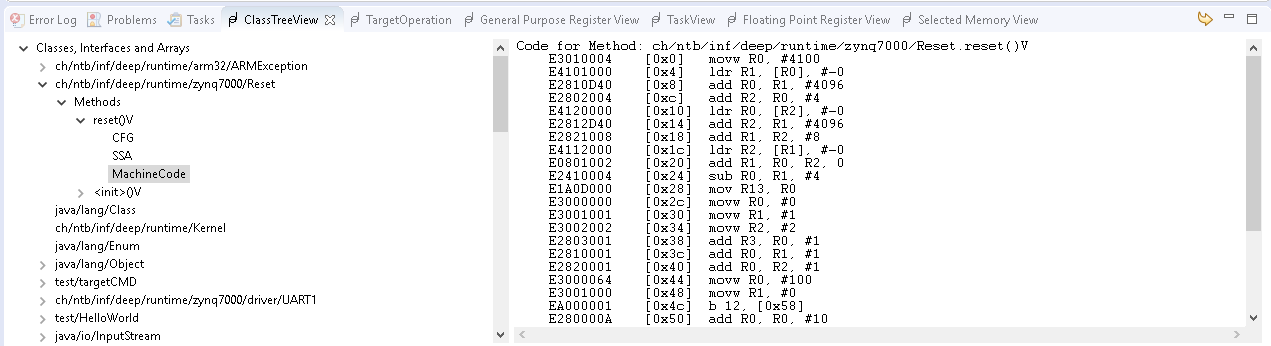
\includegraphics[width=\textwidth,height=\textheight,keepaspectratio]{images/MaschineCode_ClassTreeView_Deep.PNG}
	\caption[]{ClassTreeView mit Maschinencode der Reset-Methode in \textit{deep}}
	\label{fig:MaschineCode.ClassTreeView.Deep}
\end{figure}


\FloatBarrier

loop.S:
\lstset{language={[x86masm]Assembler}}
\begin{lstlisting}
.global _start

.org 0x000000
.text
Ltext0:

_start:
_reset:
c_entry:
movw R13, #1024

movw R0, #0
movw R1, #10
movw R2, #20
add R3, R0, #1
add R0, R1, #1
add R0, R2, #1
movw R0, #100
movw R1, #0
b CHECK_LOOP_EXIT	
START_LOOP_BODY:
add R0, R0, #10
add R1, R1, #1
CHECK_LOOP_EXIT:
cmp R1, #10
blt START_LOOP_BODY
add R1, R0, #1
add R0, R1, #1
add R1, R0, #1
add R0, R1, #1
add R1, R0, #1
b 0
\end{lstlisting}

% TODO aufgeräumt gut?
\textit{''loop.S''} im Anhang \ref{anhang:loop.S} enthält den ''aufgeräumten'' Assemblercode.
Der Code wurde mit zusätzlichen Assembler-Direktiven ergänzt.
\texttt{''c\_entry''} beschreibt den Punkt, an dem das Programm anfängt.
\texttt{''START\_LOOP\_BODY''} und \texttt{''CHECK\_LOOP\_EXIT''} sind Punkte, welche für die \textit{While-Loop} benötigt werden.

In Zeile 10 wird der Stackpointer direkt mit einer Konstante gesetzt und nicht mehr mit \textit{deep}-Konstanten ausgerechnet.
Zusätzlich kann so auch sichergestellt werden, dass der Stack in einem erlaubten Speicherbereich im OCM angelegt wird.

Die beiden Branch-Instruktionen wurden mit der korrekten Syntax ersetzt.
Als Ziel für diese Instruktionen wurden die beiden Assembler-Direktiven \texttt{''START\_LOOP\_BODY''} und \texttt{''CHECK\_LOOP\_EXIT''} verwendet.


\subsection{STABS in das Assemblerprogramm einfügen}
Um das Assemblerprogramm mit STABS zu ergänzen wurden drei verschiedene Quellen genutzt.
Das Fertige Assemblerprogramm mit STABS ist im Anhang \ref{anhang:loopWithAssembler.S} angehängt.

Die NTB-Wiki-Dokumentation\footnote{https://wiki.ntb.ch/infoportal/software/gdb/start?s[]=stabs} wurde als Ausgangslage genutzt.
Die Datei \textit{''stabs.include''} (siehe Anhang \ref{anhang:stabs.include}) konnte direkt genutzt werde.
Die Definition des Sourcecode (N\_SO) und die Definitionen der Zeilennummern (N\_SLINE) konnte ebenfalls übernommen werden.

Da die Definitionen der Variablen-Typen in der NTB-Wiki-Dokumentation nicht vollständig war, konnte sie leider nicht verwendet werden.
Alle Variablendefinitionen, Zeile 6-75, wurde aus dem disassemblierten Demoprogramm kopiert.
Bei der While-Loop ist die Definition der Source-Code-Zeile ebenfalls etwas speziell, da sie auch bei der Überprüfung der Exit-Condition stimmen muss.
Die genaue Implementation für die While-Loop wurde ebenfalls aus dem disassemblierten Demoprogramm übernommen.

Der \textit{deep}-Compiler scheint die Variablen nicht auf dem Stack zu sichern, sofern noch genügend Register frei sind.
Zusätzlich werden die Variablen in den Registern überschrieben, wenn diese im späteren Programmverlauf nicht mehr verwendet werden.
Eine Register-Variable wird mit einer Direktive vom Typ 'N\_RSYM' definiert, die auf ein bestimmtes Register zeigt.
So werden beispielsweise die Register-Variablen \texttt{x00}, \texttt{x01} und \texttt{x02} in den Zeilen 84, 89 und 94 definiert.

\lstset{language={[x86masm]Assembler},
  firstnumber=84,
  numberfirstline=true}
\begin{lstlisting}
.stabs "x00:r(0,1)",N_RSYM,0,4,0
\end{lstlisting}

\lstset{language={[x86masm]Assembler},
  firstnumber=89,
  numberfirstline=true}
\begin{lstlisting}
.stabs "x01:r(0,1)",N_RSYM,0,4,1
\end{lstlisting}

\lstset{language={[x86masm]Assembler},
  firstnumber=94,
  numberfirstline=true}
\begin{lstlisting}
.stabs "x02:r(0,1)",N_RSYM,0,4,2
\end{lstlisting}
\lstset{firstnumber=1}


Auf der Sourcecode-Zeile 11 wird die Variable \texttt{x00} um 1 inkrementiert.
Im Assemblercode sieht man, dass die Variable neu im Register 3 abgespeichert wird.
Aus diesem Grund muss die Register-Variable neu definiert werden.

\lstset{language={[x86masm]Assembler},
  firstnumber=98,
  numberfirstline=true}
\begin{lstlisting}
# x00++;
.stabn N_SLINE, 0, 11, LM11
.stabn N_LBRAC, 0, 0, LM11
.stabs "x00:r(0,1)",N_RSYM,0,4,3
LM11:
add R3, R0, #1
\end{lstlisting}
\lstset{firstnumber=1}



\subsection{Demoprogramm mit STABS kompilieren}
Das Assemblerprogramm enthält nun alle notwendigen Informationen für den Maschinencode in Form von Assemblerinstruktionen.
Die STABS ergänzen das Programm mit allen Informationen, welche der Debugger benötigt.

Mit dem Script \textit{''XXX.ps1''} im Ahang \ref{anhang:XXX} kann das Programm assembliert werden.
Die ELF-Datei \textit{''XXX''} kann dann mit dem \textit{gdb} geladen werden.



% TODO besserer titel
\section{Zybo mit \textit{gdb} verwenden}
% TODO nur hw breakpoints funktionieren
	\chapter{Debugger}

Es gibt diverse Debugger auf dem Markt.
Diese Arbeit beschränke sich aber auf den GNU-Debugger (\textit{gdb}), da unter der PGL Lizenz steht und somit eine Open Source Software ist.
Bei den meisten Linux Distributionen wird der \textit{gdb} direkt mitgeliefert und kann sofort verwendet werden.


% \section{Anwendungsbeispiel gdb auf einem Linux-System}
% Mit diesem Beispiel will ich zum einen ein kurzes Tutorial bieten um den Umgang mit dem \textit{gdb} zu lernen.
% Zum anderen will ich damit aber auch die verschiedenen Funktionen vom Debugger zeigen, damit die beschriebenen Probleme später im Kapitel besser in einen Kontext gestellt werden können.
% 
% Für dieses Tutorial verwende ich ein Linux Mint 18.1 (basierend auf einem Ubuntu 16.01).
% Solange \textit{gdb} installiert ist, ist das verwendete Betriebssystem aber nicht relevant.

\subsection{Grundlegende Funktionsweise}
Auf Linux verwendet der \textit{gdb} den System Call \textit{ptrace} (Kurzform für "process trace").
Dieser System Call erlaubt dem \textit{gdb} einen anderen Prozess zu inspizieren und zu manipulieren.
Im Hardwaredebugger, den wir später bearbeiten, verwenden wir stattdessen JTAG in Verbindung mit der Debugginghardware im Prozessor.

\subsection{Vorbereitung}
Für dieses Tutorial verwenden wir folgendes Beispielprogramm:

\lstset{language=c}
\begin{lstlisting}
#include <iostream>
using namespace std;  

int divint(int, int);  
int main() 
{ 
   int x = 5, y = 2; 
   cout << divint(x, y); 
   
   x =3; y = 0; 
   cout << divint(x, y); 
   
   return 0; 
}  

int divint(int a, int b) 
{ 
   return a / b; 
}  

\end{lstlisting}

Diese Applikation können wir jetzt Kompilieren und mit \textit{gdb} starten:\\
\shellcmd{g++ gdbTest.cpp -o gdbTest}\\
\shellcmd{gdb gdbTest}\\
\shellcmd{run}        // startet die Applikation im \textit{gdb}

\shelloutput{(gdb) run}\\
\shelloutput{Starting program: /home/mgehrig2/projects/gdbTest/gdbTest}\\
\\
Program received signal SIGFPE, Arithmetic exception.\\
0x00000000004007b5 in divint(int, int) ()\\



Obwohl die Applikation nicht mit Debug-Symbolen kompiliert wurde, wird nicht nur die Adresse des Ursprungs der Floating Point Exception angezeigt, sondern auch der Name der Methode.




% \section{Unterschied zwischen einem Software- und Hardwaredebugger}


\section{Funktionen eines Debuggers}
Ein Debugger kann verschiedene Funktionen besitzen.
Die grundlegenden Funktionen sind sehr einfach und brauchen keine grosse "Intelligenz" vom Debugger selber.

Erweiterte Funktionen erwarten vom

\section{Erstellen einer Dummy-Applikation mit Debug-Informationen}
\subsection{Vorgehen}
Das Ziel von diesem Kapitel ist es, eine Deep-Applikation zu erzeugen, die mit \textit{gdb} und \textit{OpenOCD} %TODO





\section{ELF-File}
ELF 




% ELF selber erstellen


% gdb arm toolchain





	\chapter{Ehrenwörtliche Versicherung}

	Der unterzeichnende Autor dieser Arbeit erklärt hiermit, dass er die Arbeit selbst erstellt hat,
	dass die Literaturangaben vollständig sind und der tatsächlich verwendeten Literatur entsprechen.\\
	\\
 	\\
	St. Gallen, 10. August 2018\\
    \\
    \\
    \\
  	Marcel Gehrig\\

%	\chapter{BeagleBone Black Derivat}



\section{Übersicht}
Das BeagleBone Black-Derivat ist ein identischer Nachbau zum kostengünstigen Einplatinen-Computer BeagleBone Black. Es ist sowohl von der Funktion und dem Layout her praktisch identisch, kann aber, dank dieser Arbeit, selbst nach Abkündigung durch andere Hersteller immer noch von Variosystems hergestellt werden. Dies ermöglicht eine zeitliche Verfügbarkeitsgarantie und Unabhängigkeit von anderen Herstellern.


Da der BBB eine Open Source-Hardware ist, sind die eCAD-Pläne frei erhältlich. Die offiziellen Pläne sind allerdings mit dem eCAD-Tool mit dem Namen OrCAD erstellt worden \cite{bbbOrcad}. Diese Dateien sind aber nicht mit dem Altium Designer, dem eCAD-Tool welches in dieser Arbeit und bei Variosystems verwendet wird, kompatibel. Auf der Homepage von 'Element 14', einem offiziellen Distributor des originalen BBB, sind dennoch Pläne zu finden, welche mit dem Altium Designer erstellt wurden \cite{element14AltiumBBB}. Diese Pläne beziehen sich aber noch auf die 'Revision A5B', wobei 'Revision C' die aktuelle Revision ist. Alle Änderungen von Revision 'A5B' zur Revision 'C' wurden manuell in dieser Arbeit gemacht. Das Schema für das BBB-Derivat ist im Kapitel \ref{sec:anhang_schema_bbb_derivat} angehängt.



\section{Struktur des eCAD Projektes}

\subsection{Allgemeines}
Das elektrische Schema, das PCB Layout und auch die diversen Produktionsdateien, wie zum Beispiel die Gerber-Daten, wurden mit Altium Designer erzeugt. Zusätzlich wurde ein awk-Skript verwendet, um die Pick-and-Place-Datei richtig zu formatieren. Mehr dazu im Kapitel \ref{sec:awkSkript}.

\subsection{Aufbau des Schema}
Das Elektrische Schema ist, genau wie das Schema des originalen BBB, auf folgende 11 Top-Level-Blätter verteilt:

\begin{itemize}
\item P01: Titelblatt
\item P02: Power-Management
\item P03: Prozessor 1 und JTAG Header
\item P04: Prozessor 2/3, USB und Serial
\item P05: Prozessor 3/3
\item P06: LED, Bootup-Konfiguration und Taster
\item P07: DDR3 Arbeitsspeicher
\item P08: eMMC Festspeicher
\item P09: Ethernet
\item P10: HDMI
\item P11: Stiftleisten, $\mu$SD und EEPROM
\end{itemize}

Im Folgenden wird nur noch auf die Seitennummer des Schema (P01...P11) verwiesen, und nicht mehr auf den Namen. 


\subsection{Bauteile und Bauteilbibliotheken}
Alle verwendeten Bauteile haben einen sogenannten 'Life Supplier Link'. Dieser Link verweist direkt auf die Datenbanken der Distributoren. Durch diesen Link kann die Stückliste automatisch erstellt werden. Aus der Stückliste ist direkt ersichtlich, ob das Bauteil beim jeweiligen Distributor vorrätig ist, und wie hoch der Kaufpreis es in der benötigten Menge aktuell ist.

Wenn möglich, wurde Digi-Key als Distributor gewählt. Wenn das Bauteil bei Digi-Key nicht erhältlich oder nicht vorrätig war, wurde auf Mouser oder Arrow ausgewichen. Bei Arrow funktionierte der Life-Link allerdings nicht. Aus diesem Grund wurde die Stückliste bei allen Bauteilen von Arrow manuell ergänzt. In der Stückliste sind diese manuellen Ergänzungen gelb hinterlegt.

Widerstände und Kondensatoren, welche auch in der Bauteilbibliothek von Variosystems vorhanden sind, haben einen Parameter mit dem Namen 'VS Part Number'. In diesem Parameter ist die Artikelnummer von Variosystems hinterlegt, die dem entsprechenden Standardbauteil von Variosystems entspricht.

\subsection{Output Files}
Als 'Output Files' werden im Altium Designer alle Dateien bezeichnet, welche aus dem elektrischen Schema oder dem PCB Layout erzeugt werden. Diese Dateien werden in einem 'Output Job' (BBB\_Derivat.OutJob) definiert. Dieser 'Output Job' enthält folgende Container, welche die entsprechenden Dateien erzeugt:

\begin{itemize}
\item Assembly: Erzeugt PDFs, welche beim Bestücken des PCBs hilfreich sein können.
	\begin{itemize}
	\item ASSEMBLY\_Print.pdf: Ein Plan, der bei der Positionierung der Bauteile auf dem PCB hilft
	\end{itemize}
\item Production Data: Erzeugt alle Dateien, welche für die Herstellung und Bestückung des PCBs notwendig sind.
	\begin{itemize}
	\item Pick And Place Files: Dateien für die Pick-and-Place Maschine. Mehr dazu im Kapitel \ref{sec:awkSkript}.
	\item Gerber Files: Die Gerber Daten werden für die Produktion des PCBs benötigt.
	\item NC Drill Files: Plan für die Bohrungen.
	\item Bill of Materials: Stückliste. Diese wird automatisch mit den aktuellen Informationen aus den 'Life Supplier Link' ergänzt.
	\end{itemize}
\end{itemize}

%TODO evt ergänzungen

\subsection{Pick and Place: awk Skript}\label{sec:awkSkript}
'awk' ist eine Skriptsprache, die auf einfache Weise erlaubt, strukturierten Text zu bearbeiten.

Der Altium Designer erzeugt eine Datei mit den Informationen für die Pick and Place Maschine. In dieser Datei ist unter Anderem der Designator, die Position und der Drehwinkel des Bauteils gespeichert.

Die Pick and Place Maschine von Variosystems benötigt aber je für die obere und die untere Lage eine separate Datei. Des Weiteren sollten die Artikelnummer von Variosystems für die entsprechenden Standardbauteile hinzugefügt und unnötige Informationen entfernt werden. Diese Aufgabe wurde mit dem awk-Skript 'Pick-n-Place-Separator.awk' (siehe Anhang Kapitel XXX) automatisiert.
%TODO auf angehängtes Skript XXX verweisen

Bei der Bestückung bei Variosystems hat sich aber gezeigt, dass diese Dateien gar nicht verwendet wurden. Die Technische Abteilung von Variosystems hat die Pick and Place Datei selber aus der PCB ASCII Datei (*.PcbDoc) erstellt. Das PCB wird normalerweise in einem binären Format gespeichert. Um das PCB-Layout als eine ASCII-Datei zu speichern, muss diese mit der Funktion 'Speichern unter...' speziell erzeugt werden.

\section{Upgrade auf Revision C}\label{sec:upgrade_rev_c}
Im Folgenden werden alle Änderungen aufgelistet, welche gemacht wurden, um die Pläne von 'Element 14' an die 'Revision C' anzupassen. Die zusätzlichen Bauteile wurden auf dem PCB an den gleichen Position platziert, wie auf dem originalen BBB.

\begin{itemize}
\item A5C: 
%Diese Änderungen wurden wegen Produktionsfehler, verursacht von Unterschieden in den Widerständen, gemacht.
	\begin{itemize}
	\item R46, R47 und R48 auf 0$\Omega$ geändert.
	\item R45 auf 22$\Omega$ geändert.	
	\end{itemize}
\item A6:
	\begin{itemize}
	\item Der 'Enable' Eingang des VDD\_3V3B Spannungsregler (U4) ist neu mit VDD\_3V3A verbunden.
	\item AND-Gate (U16) hinzugefügt.	
	\item Optionaler 0$\Omega$ Widerstand (R29) hinzugefügt.	
	\end{itemize}
\item A6A:
	\begin{itemize}
	\item Optionaler 0$\Omega$ Widerstand (R30) hinzugefügt.
	\item C106 auf 1$\mu$F geändert.
	\item C24 auf 2.2$\mu$F geändert.
	\item R8 auf 'Bestücken' und R9 auf 'Nicht bestücken' gesetzt.
	\end{itemize}
\item B:
	\begin{itemize}
	\item Der Prozessor (U5) ausgewechselt. Neue Modellnummer: AM3358BZCZ100.	
	\end{itemize}
\item C:
	\begin{itemize}
	\item Den eMMC Speicher (U13) von 2GB auf 4GB erhöht.
	\end{itemize}
\end{itemize}



\section{Elektrisches Schema}
Die Hardware und die Funktion des BBB, und somit auch des BBB-Derivates, wird im 'System Reference Manual (SRM) \cite{adafruitSRM} ausgiebig beschrieben. Aus diesem Grund wird im Folgenden nur auf Aspekte eingegangen, die im Zusammenhang mit dem ComCape interessant sind, oder nicht im SRM erwähnt werden.


\subsection{Power-Management}
Der Power-Management-IC TPS65217\textit{CRSLR} (U2) stellt zusammen mit dem TL5209 (U4) die verschiedenen Spannungspegel zur Verfügung. Der TPS65217\textit{CRSLR} (U2) ist dabei speziell auf den verwendeten Prozessor AM3358BZCZ100 (U5) und den DDR3 Arbeitsspeicher abgestimmt.

Das BBB-Derivat kann über die Mini-USB-Buchse oder mit einem separaten 5V-Netzteil betrieben werden. Wird es allerdings zusammen mit dem ComCape genutzt, ist es unbedingt notwendig, dass ein Netzteil mit mindestens 2A verwendet wird. Die Spannungsversorgung nur über USB ist dann nicht ausreichend.


Die verschiedenen Versorgungsspannungen sind in Tabelle \ref{tab:versorgungsspannungen} zusammengefasst. Im SRM\cite{adafruitSRM} werden diese noch genauer beschrieben.

\begin{table}

    \begin{tabular}{ | l | l | l | p{7cm} |}
    \hline
    \textbf{Name}		& \textbf{Spannung} 	& \textbf{Max. Strom} 	& \textbf{Beschreibung} \\ \hline
    
    VRTC		& 1.8V		& 250mA	 		& Wird beim Powerup als erstes aktiviert. Speist die IO Spannung des Power-Management-IC und die Echtzeituhr des Prozessors.\\ \hline    
    
    VDD\_3V3A 	& 3.3V 		& 400mA 		&  3.3V Stromversorgung für den Prozessor. Da die Stromstärke aber nicht für die Peripherie ausreicht, ist ein zusätzlicher, diskreter Spannungsregler verbaut. Siehe 3V3B.\\ \hline
    
    VDD\_3V3B	& 3.3V 		& 500mA 		& 3.3V Stromversorgung für Peripherie. Dazu gehören: JTAG, UART0, eMMC, Ethernet, HDMI und die $\mu$SD. Mit dem Pin \textit{AI7} des Prozessors (U5) kann diese Spannung gemessen werden. Diese Spannung wird über die Stiftleiste geführt, und kann für die Signalpegelwandler verwendet werden.\\ \hline
    
    VDD\_5V		& 5V 		& 2'000mA 		& 5V Spannung direkt vom externen Netzgerät. Die maximale Stromstärke wird auch vom verwendeten Netzgerät begrenzt. Dabei darf nicht vergessen werden, dass der BBB indirekt ebenfalls über das externe Netzgerät gespeist wird, und dieses belastet. Diese Spannung ist nicht präsent, wenn der BBB nur über USB und nicht mit einem externen Netzgerät gespeist wir. Ein einzelner Pin darf maximal mit 1'000mA belastet werden. Diese Spannung wird über zwei Pins zum Cape geführt.\\ \hline
    
    SYS\_5V		& 5V 		& 500mA 		& Diese 5V werden vom Power-Management IC von der USB-Spannung oder vom externen Netzgerät generiert. Diese Spannung wird vom Power-Management-IC selbst verwendet.\\ \hline
    
    VDD\_1V8	& 1.8V 		& 400mA 		& Exklusiv für den Prozessor und den HDMI Framer.\\ \hline
    
    VDD\_CORE	& 1.1V 		& 1'200mA 		& Exklusiv für den Prozessor.\\ \hline
    
    VDD\_MPU	& 1.1V 		& 1'200mA 		& Exklusiv für den Prozessor.\\ \hline
    
    VDD\_CORE	& 1.5V 		& 1'200mA 		& Exklusiv für den DDR3. Kann für DDR3L auf 1.35V gesenkt werden.\\ \hline
    
    
    \end{tabular}
    \caption{Versorgungsspannungen des BBB}
    \label{tab:versorgungsspannungen}

\end{table}



\subsection{Spannungspegel für die digitale Kommunikation}
Die digitalen IOs des Prozessors können grundsätzlich mit 1.8V oder mit 3.3V gespeist werden. Auf dem BBB-Derivat werden sie mit 3.3V betrieben. Aus diesem Grund haben die digitalen IOs einen TTL-Spannungspegel von 3.3V. Dieser Spannungspegel wird von der $\mu$SD-Karte benötigt.

\subsection{Power-Up-Sequence}
Damit der BBB nicht beschädigt wird, müssen die verschiedenen Spannungsversorgungen in der richtigen Reihenfolge gestartet werden. Dies wird bereits vom Power-Management-IC übernommen.

Im SRM \cite{adafruitSRM} auf Seite 113 wird darauf hingewiesen, dass keine Spannungen an die IO-Pins des Prozessors angelegt werden, bevor die \textit{VDD\_3V3B} Spannungsversorgung gestartet wird. Das BLE-Modul wird über diese Spannungsversorgung gespeist. So ist es nicht möglich, das BLE-Modul eine Spannung anlegt, bevor \textit{VDD\_3V3B} gestartet wird.
Das WLAN-Modul und das GSM-Modul sind über einen Spannungspegelwandler (\textit{TXS0108E}) mit dem Prozessor verbunden. Die 3.3V-Seite des Pegelwandlers, welche mit dem Prozessor verbunden ist, wird ebenfalls über die \textit{VDD\_3V3B} Spannungsversorgung gespeist. So wird verhindert, dass beim Prozessor eine Spannung anliegt, bevor \textit{VDD\_3V3B} gestartet ist.

Auch \textit{VDD\_5V} darf nicht belastet werden, bevor \textit{VDD\_3V3B} gestartet ist. Dies ist aber kein Problem, da \textit{VDD\_5V} auf dem ComCape nicht verwendet wird.

\subsection{Optionale Komponenten}
Für die Kernfunktion des BBB, also booten und ausführen des Betriebssystems, sind nicht alle verbauten Bauteile notwendig. Für bestimmte Funktionen werden diese zusätzlichen Bauteile aber gebraucht. Im Schema des BBB-Derivats sind diese Bauteile mit einer grünen Strich-Punkt-Linie umrandet, und mit grüner Schrift betitelt. Alle anderen Komponenten sind für das Ausführen eines Betriebssystems notwendig. Wenn eine Funktion auf dem BBB-Derivat nicht benötigt wird, kann auf alle Bauteile in der Umrahmung verzichtet werden. Diese optionalen Funktionen werden in der Tabelle \ref{tab:optionaleFunktionen} aufgelistet.


\begin{table}
    \begin{tabular}{ | p{2.5cm} | l | p{9.5cm} |}
    \hline
    \textbf{Funktion}		& \textbf{Blatt} 	& \textbf{Funktion} \\ \hline
    
    Clock HDMI Framer		& P03		& Dieser Clock wird nur für die HDMI-Schnittstelle benötigt (P10 'HDMI').\\ \hline   
    
    Clcok McASP				& P03		& Dieser Clock wird benötigt, wenn die McASP Schnittstelle verwendet wird.\\ \hline   
    
    JTAG Schnittstelle		& P03		& Bietet einen Header für die JTAG-Verbindung zum Prozessor. Diese Schnittstelle wird auch auf dem originalen BBB nicht bestückt.\\ \hline  
    
    UART 0 Debugschnittstelle	& P04		& Eine elektrisch isolierte UART Verbindung (UART0), auf die über die Stiftleisten J1 zugegriffen werden kann. Diese Verbindung kann auch als Debugschnittstelle verwendet werden. \\ \hline      
    
    USB Host				& P04		& USB Host Funktionalität des BBB.\\ \hline    
    
    USB PC Connector		& P04		& Über die USB-Mini-Buchse kann der BBB mit einem PC verbunden werden. Durch diese Verbindung kann der BBB mit Spannung versorgt werden. Zusätzlich kann über diese Verbindung von einem separatem PC auf die Entwicklungsumgebung und die Daten auf dem BBB zugegriffen werden.\\ \hline    
    
    User LED				& P06		& LEDs, die den Status des BBB anzeigen, und auch individuell Programmiert werden können.\\ \hline  
    
    eMMC					& P08		& Dies ist der 4GB grosse Festspeicher des BBB. Das Betriebssystem kann allerdings auch direkt von der $\mu$SD gebootet werden. Das System läuft aber deutlich schneller, wenn es vom eMMC gestartet wird. \\ \hline 
    
    Ethernet				& P09		& Ethernet-Verbindung inklusive PHY und Buchse. Der MAC ist im Prozessor integriert.\\ \hline    
    
    HDMI					& P10		& Der HDMI-Framer wandelt das LCD-Signal vom BBB in ein HDMI-kompatibles Signal um, welches von einem normalen, HDMI-fähigen Monitor wiedergegeben werden kann. Dies funktioniert aber nur, wenn die LCD-Pins des BBB nicht für einen LCD oder andere Funktionen verwendet werden. Zusätzlich wird noch das Taktsignal für den HDMI benötigt (siehe P03 'Clock HDMI Framer'). \\ \hline   
    
    LCD or HDMI				& P10		& Diese Kondensatoren werden nur benötigt, wenn entweder ein externer LCD angeschlossen wird, oder wenn der HDMI Ausgang benutzt wird.\\ \hline 
    
    Expansion Header& P11		& Über die beiden Stiftleisten können die diversen Capes, unter anderem auch das ComCape, verbunden werden.\\ \hline 

    \end{tabular}
	\caption{Optionale Funktionen des BBB}
	\label{tab:optionaleFunktionen}
\end{table}


\subsection{$\mu$SD}
Das Betriebssystem kann wahlweise von der $\mu$SD oder vom eMMC aus gebootet werden. Eine $\mu$SD Karte ist eine „Mikro-Secure-Digital Flash Speicherkarte“ welche auch in vielen Smartphones als Erweiterung für den internen Speicher dient. Um den fabrikneuen und unbeschriebenen eMMC mit einem bootfähigen Betriebssystem zu beschreiben, wird eine $\mu$SD mit einem speziellen Image benötigt. Auf dieses Thema wird im Softwareteil der Dokumentation im Kapitel [XXX] noch weiter eingegangen.
%TODO Kapitel EGEMEN


\subsection{DDR3L RAM}
Der DDR3L SDRAM ist ein RAM, der mit einer Spannungsversorgung von 1.35V betrieben werden kann. Im BBB-Derivat, wie auch beim originalen BBB, wird er aber im Rückwärtskompatibilitätsmodus  mit 1.5V betrieben. Dies wurde so gelöst, damit am originalen BBB Design möglichst wenig verändert werden musste.


\subsection{I$^2$C EEPROM}
Auf dem BBB befindet sich ein EEPROM, der über I$^2$C angesprochen werden kann. Für das Booten des Betriebssystems sind bestimmte Informationen auf dem EEPROM notwendig. Ohne diese Informationen startet der BBB nicht.

Zum Programmieren der 5 EEPROMS für die 5 Prototypen wurde ein Arduino-Klon mit dem Namen 'MINI-AT Board' verwendet. Zusätzlich wurde ein SchmartBoard\textsuperscript{TM} verwendet. Auf dem SchmartBoard\textsuperscript{TM} sind die beiden Pull-Up Widerstände, welche für den I$^2$C benötigt werden, aufgelötet. Zusätzlich bietet es Platz um die EEPROMS aufzulöten. Ein SchmartBoard\textsuperscript{TM} ist ein Prototypen-PCB, welches speziell dafür ausgelegt ist, um SMT Bauteile von Hand aufzulöten. In Abbildung XXX ist das 'MINI-AT Board' mit dem SchmartBoard\textsuperscript{TM} zu sehen. Abbildung YYY zeigt die elektrische Verdrahtung des Arduino-Klons um ein EEPROM zu programmieren.

Wie der EEPROM genau programmiert wurde, wird im Softwareteil im Kapitel XXX beschrieben.

%TODO Verweis auf SW
%TODO Bild Audrino + Verweis XXX
%TODO Bild El Schema Audrino EEPROM YYY


\subsection{Belegung der Pinheader}
Die verwendete Pinbelegung der Erweiterungs-Stiftleisten P8 und P9 ist im Anhang \ref{sec:anhang_pinbelegung} dokumentiert. Alternative Pinbelegungen sind im 'System Reference Manual'\cite{adafruitSRM}  des BBB dokumentiert.




\section{Aufbau des PCB}\label{aufbauPCB}
Für digitale Hochgeschwindigkeitskommunikation spielt die Wellenimpedanz der Leiterbahnen eine grosse Rolle. Die Impedanz wird durch den Lagenaufbau des PCBs, aber auch durch die Breite der Leiterbahnen definiert. Man unterscheidet dabei zwischen 'Single-Ended' und 'Differential Pair'. Bei einem 'Differential Pair' werden zwei Leiterbahnen benötigt, die in einem definiertem Abstand parallel zueinander geführt werden.

In diesem Layout kommen die Impedanzen Single '50$\Omega$', 'Differential 90$\Omega$' und 'Differential 100$\Omega$' vor. Wenn das Layout des PCB mit dem Altium Designer geöffnet wird, sind die Leiterbahnen der verschiedenen Impedanzen in den Netklassen 'Single\_50', 'Diff\_90' und 'Diff\_100' sortiert.

Die PCBs wurden speziell mit Impedanzkontrolle bestellt, damit eine definierte Impedanz gewährleistet werden konnte. Auf Anfrage hat der Hersteller, Multi Circuit Borads, eine Tabelle mit dem Lagenaufbau und den benötigten Leiterbahnbreiten für die gewünschten Impedanzen (siehe Abbildung \ref{LagenaufbauBB}) geschickt.

In Abbildung \ref{LagenaufbauBB} ist ebenfalls zu sehen, dass die benötigte Leiterbahnbreite für eine bestimmte Impedanz für die Innenlagen anders ist, als für die Aussenlagen. Alle Leiterbahnen, welche eine vordefinierte Impedanz und somit auch eine genau definierte Breite benötigen, wurden auf dem PCB Layout des BBB-Derivats angepasst.

Das PCB des BBB hat 6 Lagen. \textit{TOP} und \textit{BOTTOM} sind die beiden Aussenlagen. Die zweite Lage, \textit{L2}, ist komplett gefüllt mit einer GND-Fläche. Die beiden innersten Lagen, \textit{L3} und \textit{L4}, werden für Leiterbahnen verwendet. Die 5. Lage, \textit{L5}, ist für die Spannungsversorgung reserviert.


\begin{figure}[!ht]
\centering
\includegraphics[angle=0,width=14cm]{images/LagenaufbauBB.jpg}
\caption{Lagenaufbau und Impedanzen des BBB}
\label{LagenaufbauBB}
\end{figure}


\section{Layout des PCB}

\subsection{Änderungen}
Am Layout des PCB, welches von der 'Element 14'-Homepage stammt, wurden folgende Änderungen vorgenommen:

%TODO detailierter; evt. Bilder
\begin{itemize}
\item Die Leiterbahnbreiten für die kontrollierten Impedanzen wurden entsprechend angepasst
\item Alle Änderungen für das Upgrade auf die Revision C (siehe \ref{sec:upgrade_rev_c}).
\item Der obere und unter Beschriftungsdruck wurde so angeordnet, dass die Designatoren gut sortiert und lesbar sind
\end{itemize}


\subsection{Kritische Stellen des Layouts}
Bei digitalen Hochgeschwindigkeitsübertragungen ist die Signalintegrität von grosser Bedeutung. Die Signalintegrität beschreibt, wie gut das gesendete Signal des Senders mit dem Signal übereinstimmt, welches der Empfänger am anderen Ende der Leitung empfängt. Wenn die Signalintegrität zu klein ist, kann es zu Datenverlusten führen. Dieser Datenverlust kann dazu führen, dass die Datenverbindung nicht mehr brauchbar ist. Wenn z.B. die Signalintegrität der Verbindung zwischen dem Prozessor und dem RAM zu schlecht ist, kann der Prozessor den RAM gar nicht mehr nutzen. Da der BBB ohne RAM nicht lauffähig ist, muss dies unbedingt verhindert werden.

Für eine gute Signalintegrität muss unter anderem die Impedanz der Leiterbahnen stimmen. Dieses Thema wurde bereits im Kapitel \ref{aufbauPCB} diskutiert. Zusätzlich müssen alle Leiterbahnen gleich lang sein, damit alle Signale gleichzeitig ankommen. Elektromagnetische Störungen von aussen können die Signalintegrität ebenfalls beeinflussen.

In Abbildung \ref{kritischeStellenBBB} sind alle Leiterbahnen, bei denen die Signalintegrität ein kritischer Faktor sein könnte, rot eingerahmt. Ohne detailliertes Wissen über digitale Signalintegrität, sollte das PCB Layout in diesem Bereich nicht geändert werden.

\begin{figure}[!ht]
\centering
\includegraphics[angle=0,height=5cm]{images/BBB_kritische_stellen.png}
\caption{Kritische Stellen des BBB}
\label{kritischeStellenBBB}
\end{figure}




\section{Produktion der Prototypen}


\subsection{Vorgehen}
Die PCBs wurden von der Firma 'multi-cb' gefertigt. Die fertigen PCB sind dann beim Industriepartner Variosystems bestückt worden. Es wurden 10 PCBs bestellt, fünf davon sind bestückt worden.

Bei einer Bestückung durchläuft das PCB mehrere Stationen. Zuerst wird die Lötpaste auf das PCB aufgetragen. Anschliessend werden alle Bauteile durch einen Pick-and-Place-Roboter auf dem PCB platziert. In einem Reflow-Ofen wird dann das ganze PCB inklusive Bauteile und Lötpaste erhitzt, so dass die Bauteile endgültig mit dem PCB verlötet werden. Diese Schritte werden einmal für die Oberseite und einmal für die Unterseite ausgeführt. Mit einem Röntgengerät können dann auch die Lötstellen unter einem Bauteil kontrolliert werden.

Aufgrund von Firmenrichtlinen konnten bei der Bestückung leider keine Fotos von der Produktionsstrasse geschossen werden.


\subsection{Lötpaste}
Bei der ersten Station der Produktion wurde zuerst eine Lötpastenmaske aus dünnem Stahlblech genau über das PCB gelegt. Die Ausschnitte des Bleches entsprechen dem Layer \textit{Top Paste} und \textit{Bottom Paste} im PCB Dokument. Über diese Maske wurde feinkörnige, bleifreie Lötpaste gestrichen, die bei den Aussparungen der Maske auf dem PCB haften bleibt.

Der Nutzenrand des PCBs (siehe Abbildung XXX) war hier von grossem Vorteil. Dank diesem Rand konnte das PCB problemlos auf dem Förderband fixiert werden, ohne dass Lötstellen verdeckt werden. Nachdem die Lötpaste aufgetragen wurde, wurde das PCB auf einem Förderband zum Pick and Place Roboter transportiert.
%TODO Foto PC mit Nutzenrand


\subsection{Pick-and-Place-Roboter}
Im Pick-and-Place-Roboter wurden alle SMT Bauteile bestückt. Der Roboter platziert dabei alle SMT Bauteile auf dem PCB, durch die Lötpaste schwach auf dem PCB haften.

Das Einrichten der Maschine war ein sehr grosser Initialaufwand. Nachdem der Roboter aber richtig eingestellt wurde, ging das Bestücken zügig und ohne grössere Probleme voran. Aus diesem Grund ist diese Maschine nur bei grossen Stückzahlen effizient. 

Der Roboter hat leider immer wieder Bauteile verloren, die mühsam in der Maschine gesucht werden mussten. Da nicht alle Bauteile wieder gefunden werden konnten, musste eine HDMI-Schutzdiode (D6) und drei LEDs (D1, D2 und D3) nachbestellt und nachträglich von Hand aufgelötet werden.

Beim Bestücken wurde festgestellt, dass die Mini-USB Buchse (P4) nicht genau den richtigen Footprint hatte. Dieser war aber ähnlich genug, dass die Buchse trotzdem aufgelötet werden konnte. Der Footprint des $\mu$SD-Kartenhalters (P10) war ebenfalls fehlerhaft und konnte nicht aufgelötet werden. Diese Bauteile wurden anschliessend im eCAD Projekt mit den entsprechenden Bauteilen mit den richtigen Footprints ersetzt. Die $\mu$SD Kartenhalter wurden nachbestellt und von Hand eingelötet.


\subsection{Reflow Ofen}
Das bestückte PCB wurde auf dem Förderband durch den Reflow-Ofen geführt. Der Ofen hatte verschiedene Temperaturzonen, um eine optimale Lötung zu ermöglichen. Es wurde ein Standard-Temperaturprofil für 6-Lagige PCBs verwendet. Das verwendete Temperaturprofil findet sich im Anhang unter dem Kapitel \ref{sec:anhang_reflowofen_temeperaturprofil}.


\subsection{THT Bauteile}
Die THT Bauteile können nicht mit dem Roboter bestückt werden und müssen von Hand eingesteckt werden. Diese Bauteile können dann aber automatisiert mit einer Selektiv-Lötanlage gelötet werden. Im Rahmen dieser Arbeit wurden allerdings alle THT Bauteile der fünf Prototypen von Hand eingelötet.

Die Bohrungen für die beiden 46-Pin-Header waren zu klein. Es wurden 46-Pin-Header mit kleineren Pins nachbestellt und anschliessend von Hand bestückt und gelötet. Das eCAD Projekt wurde entsprechend ergänzt.


\subsection{Röntgengerät}
Viele Bauteile haben an der Unterseite Lötstellen, die von Auge unmöglich zu kontrollieren sind. Mit einem Röntgengerät liessen sich diese Stellen aber problemlos von allen Seiten durchleuchten. Dabei wurde neben der Position des Bauteils auch die Qualität der Lötstellen kontrolliert. Für ein ungeübtes Auge ist es allerdings kaum ersichtlich, ob eine Lötstelle gut oder schlecht ist. Der Operator vor Ort konnte dies aber in einem kurzen Augenblick feststellen. Das Bild in Abbildung \ref{fig:roentgenbildProzessor} wurde mit einem Röntgengerät gemacht und zeigt den Prozessor (U5) und den LAN-Chip (U14) im Hintergrund. Im Anhang XXX sind noch weitere Röntgenbilder angehängt.

%TODO Anhang Röntgenbilder

Zur Qualitätskontrolle wurde der erste Prototyp mit dem Röntgengerät durchleuchtet. Die Röntgenbilder zeigten, dass alle Lötstellen in Ordnung waren und die Bauteile alle richtig platziert wurden.

\begin{figure}[!ht]
\centering
\includegraphics[angle=0,height=10cm]{images/Roentgenbild_U5_2.jpg}
\caption{Röntgenbild vom Prozessor}
\label{fig:roentgenbildProzessor}
\end{figure}



%	\chapter{ComCape}


\section{Übersicht}
Das ComCape, oder Communication Cape, ist eine zusätzliche Platine, welche sich auf den originalen BeagleBone Black oder auf das BeagleBone-Derivat stecken lässt. Ein Cape ist eine Platine, die eigens als Erweiterung für den BeagleBone entwickelt wurde. Solche Capes können den BBB zum Beispiel mit WLAN-Funktionalität erweitern und sind auch kommerziell erhältlich.

Das ComCape ist speziell für die Firma Variosystems entwickelt worden. Es erweitert den BBB, im Gegensatz zu den bereits erhältlichen Capes, um mehrere Funktionen:

\begin{itemize}
\item WLAN: Kabelloses Internet via Wireless LAN
\item GSM: Kabelloses Internet über das mobile Internet
\item BLE: Ermöglicht dem BBB eine drahtlose Verbindung über Bluetooth Low Energy
\item LCD: Über einen Flachbandstecker kann ein LCD mit kapazitivem Multi-Touch angeschlossen werden
\end{itemize}



\section{Allgemeiner Aufbau des ComCape}

\subsection{Elektrisches Schema}
Wie auch der BBB ist das ComCape auf 7 Top-Level Blätter verteilt:

\begin{itemize}
\item P01: Titelblatt
\item P02: WLAN 1/2
\item P03: WLAN 2/2
\item P04: GSM 1/2
\item P05: GSM 2/2
\item P06: BLE
\item P07: Stiftleiste und LCD-Stecker
\end{itemize}

Im Folgenden wird nur noch auf die Seitennummer des Schema (P01...P07) verwiesen, und nicht mehr auf den Namen.

Für alle nicht benutzten Pins der Bauteile wurden Testpunkte hinzugefügt, damit diese auch nachträglich noch zugänglich sind.

Alle Signale, die zum BBB führen, sind über einen 0$\Omega$ Widerstand geführt. So können alle Bauteile elektrisch vom BBB getrennt werden. Dies kann besonders nützlich sein, wenn ein Teil des ComCapes getrennt von dem Rest getestet werden will.

%Alle Designatoren von P02 starten mit 1, die von P03 mit 50, die Designatoren von P04 mit 100 u
%TODO Designatoren beschreiben

\section{Layout PCB}
Das PCB ist in drei Teile aufgeteilt. Auf dem unteren Teil befinden sich ausschliesslich Bauteile für das GSM, während der Mittlere Teil für WLAN-Bauteile reserviert ist. Im oberen Teil befinden sich neben dem Stecker für den LCD auch noch die Komponenten für das Bluetooth Modul.

Das Bluetooth-, das WLAN- und das GSM-Modul haben auch auf der Unterseite des ChipgehäuseS Pins, die gelötet werden müssen. Es ist nicht möglich, diese Bauteile von Hand zu löten. Aus diesem Grund wurden alle Bauteile auf der oberen Seite des PCBs im Reflow-Ofen gelötet. Für den Prototypenbau wurden die Bauteile auf der unteren Seite von Hand gelötet. Beim Erstellen des PCB-Layouts wurde darauf geachtet, dass möglichst viele Bauteile auf der oberen Seite platziert wurden. Zusätzlich wurde darauf geachtet, dass die linearen Spannungsregler, welche viel Abwärme produzieren, für die bessere Wärmeabgabe ebenfalls auf der oberen Seite platziert wurden. Die drei Module befinden sich ebenfalls auf der oberen Seite des PCBs.


\subsection{Grösse und Form des PCB}
Das ComCape sollte nicht grösser sein, als das LCD. Wenn man das LCD im Hochformat über das ComCape legt, ist das Cape aus diesem Grund gleich breit wie das LCD. Oben und unten wurde das Cape um je 1cm verlängert, um noch Befestigungsbohrungen platzieren zu können.

Da beim BBB die Ethernet-Buchse sehr hoch ist, hat das Cape auf der linken Seite eine Aussparung für diese Buchse. Zusätzlich ist die obere Hälfte des ComCapes schmaler, damit die Taster S1 und S3 vom BBB besser zugänglich sind. Anhang \ref{sec:anhang_befestigungsbohrungen} zeigt den Umriss des ComCapes und die Vermassung der Befestigungsbohrungen.



\section{Wirless LAN}
Für das Wireless LAN wurde das WL1835 Modul von Texas Instruments verwendet.

Für den BBB existiert bereits ein WLAN-Cape, welches gekauft werden kann. Auf diesem Cape ist ein WL1835 Modul verbaut. Das elektrische Schema und die Gerberdaten von diesem Cape sind frei erhältlich\cite{boardZooWLANCape}. Aus diesen Gründen haben wir das 'WL1835MOD W/ Chip Antenna' Cape als Referenzdesign verwendet.

%TODO Bild WLAN Cape


\subsection{Stromversorgung}
Die VDD\_3V3B Spannungsversorgung vom BBB wird für die prozessorseitige Spannungsversorgung des Spannungspegelwandlers verwendet.

Für die 3.3V-Spannungsversorgung wurde der gleiche lineare Spannungsregler verwendet, wie im Referenzdesign. Dieser Regler kann bis zu 1.5A liefern. Der effektive Strombedarf des Moduls ist abhängig vom Betriebsmodus und lässt sich nur schwer einschätzen. Deshalb wurde derselbe, vermutlich überdimensionierte, Spannungsregler wie im Referenzdesign verwendet. Der effektive Dauer- und Spitzen- Strom lässt sich im Betrieb mit einem Messwiderstand und einem Oszilloskop über dem Steckkontakt 'X1' messen.

Die 1.8V-Spannungsversorgung wird nur für die digitale Kommunikation verwendet. Aus diesem Grund wurde der 0.4A-Spannungsregler, welcher im Referenzdesign verwendet wird, mit einem 0.15A-Spannungsregler ersetzt, der auch in der Standardbibliothek von Variosystems zu finden ist. Auch bei dieser Versorgung lässt sich der effektive Strombedarf über den Steckkontakt 'X2' messen.

\subsection{Antenne}
Das ComCape unterstützt von der Hardware her zwei Antennen. In der Software wird aber nur eine unterstützt. Mehr dazu im Kapitel \ref{sec:wlan_varianten} weiter unten.

Bei der Antenne 1, welche gleichzeitig für WLAN und Bluetooth (ist in der Software nicht implementiert) genutzt wird, kann entweder die Kombination aus Chip- und PCB- Antenne oder eine externe Antenne verwendet werden. Wenn die externe Antenne verwendet werden soll, muss C54 eingelötet sein. Soll die PCB Antenne verwendet werden, muss C54 wieder ausgelötet und stattdessen C55 eingelötet werden.

Die externe Antenne kann über eine U.FL-Buchse angeschlossen werden.

Das PCB-Layout für die Chipantenne wurde aus dem Datenblatt der Chipantenne kopiert.

Für die Verbindung zwischen dem Modul und den Antennen wird eine Übertragungsleitung mit einer Wellenimpedanz vom 50$\Omega$ benötigt. Im Hardware User Guide von Telit[XXX] wird eine Übertragungsleitung mit den Massen, wie in Abbildung \ref{50OhmTransmissionLine} empfohlen. Berechnungen mit der Software 'txLine' haben gezeigt, dass sich die Wellenimpedanz nicht signifikant ändert, wenn diverse Masse, wie zum Beispiel die Dicke des PCB oder die Dielektrizitätskonstante des Dielektrikums, sich um 10\% ändern. Aus diesem Grund kann bei der Herstellung des PCB auf eine kontrollierte Impedanz verzichtet werden.

%TODO Quelle HW userguide Telit
%TODO Berechnungen

\begin{figure}[!ht]
\centering
\includegraphics[angle=0,height=8cm]{images/50OhmTransmissionLine.jpg}
\caption{50$\Omega$ Übertragungsleitung}
\label{50OhmTransmissionLine}
\end{figure}


\subsection{32kHz Taktsignal}
Das Modul benötigt einen 32,768kHz Takt. Je nachdem, welche Widerstände eingelötet werden, können verschiedene Quellen für den Takt ausgewählt werden. Da bei der Planung des Capes nicht klar war, welche der Varianten funktionieren würde, sind alle drei Varianten auf dem Cape verwirklicht.

\textbf{R32: Lokaler Oszillator}: Der Oszillator erzeugt auf dem Cape einen 32kHz Takt und wird sonst nirgends verwendet. Dies ist die Standardvariante, da sie auch im Referenzdesign verwendet wird, und am wahrscheinlichsten funktioniert. Allerdings ist dieser Oszillator relativ teuer.

\textbf{R24: Von BBB erzeugt, mit Pegelwandler}: Diese Variante nutzt das Taktsignal, welches vom BBB erzeugt wird. Das 3.3V Signal wird dann mit einem TXS0108E auf 1.8V gewandelt. Ungünstiger weise wird dafür extra ein separater Pegelwandler benötigt.

\textbf{R28: Von BBB erzeugt, mit Spannungsteiler}: Auch diese Variante nutzt den Takt, der vom VBB erzeugt wird. Der Spannungspegel wird diesmal aber mit einem einfachen Spannungsteiler aus zwei Widerständen auf 1.8V gebracht. Das WLAN-Modul hat beim Eingang für dieses Taktsignal einen Eingangswiderstand von 1M$\Omega$\footnote{Quelle: Datenblatt WL1835MOD Seite 11}[XXX] und kann deshalb für diese Berechnung vernachlässigt werden. Wenn diese Variante funktioniert, ist sie am günstigsten und den anderen beiden vorzuziehen.
$$U_{out} =  3.3V * \dfrac{R29}{R29+R27} = 3.3V * \dfrac{4.7k\Omega}{4.7k\Omega+3.9k\Omega} = 1.80V$$

%TODO Quelle [XXX]

\subsection{Digitale Verbindung zum Prozessor}
Die WLAN-Daten werden über eienen SDIO Bus zum Prozessor übertragen. Der Spannungspegel wird dabei mit zwei TXS0108E Spannungswandlern von den 1.8V des Moduls auf 3.3V für den Prozessor gewandelt. Dieser Wandler funktioniert auf beide Richtungen, so dass auch Signale vom Prozessor zum WLAN-Modul auf den richtigen Pegel gewandelt werden.

Auf den zweiten TXS0108E kann verzichtet werden, wenn das 32kHz Taktsignal nicht vom VBB erzeugt wird.

\subsection{Varianten}\label{sec:wlan_varianten}
Das WL1835 Modul unterstützt neben einem Design mit zwei Antennen auch noch Bluetooth. Im ComCape wird Bluetooth und die zweite Antenne aber von der Software nicht unterstützt. Von der Hardware ist aber alles Nötige vorhanden. Die zweite Antenne könnte für MIMO oder eine MRC Konfiguration genutzt werden. MIMO steht für 'Multiple Input Multiple Output', damit kann im Vergleich zu einem Design mit einer Antenne (SISO = Single Input Single Output) die Bandbreite erhöht werden. Mit MRC oder 'Maximum Ratio Combining' kann die Reichweite des Signals erhöht werden.

Es existieren zum WL1835 pinkompatible Module, welche ein Design mit zwei Antennen, Bluetooth oder beides nicht unterstützen. In der Tabelle \ref{tab:wlanVarianten} sind alle vier Module und deren Funktionen aufgelistet.

\begin{table}

    \begin{tabular}{ | c | c | c | c | c |}
    \hline
    \textbf{Modul}		& \textbf{2.4-GHZ SISO}	& \textbf{2.4-GHZ MIMO}	& \textbf{2.4-GHZ MRC}	& \textbf{Bluetooth} \\ \hline
    
     WL1835MOD	& X				& X	 			& X				& X \\ \hline    
    
     WL1831MOD	& X				&	 			& 				& X \\ \hline  
    
     WL1805MOD	& X				& X	 			& X				&  \\ \hline  
    
     WL1801MOD	& X				& 	 			& 				&  \\ \hline  
    
    
    \end{tabular}
\caption{Varianten des WLAN Moduls}
\label{tab:wlanVarianten}
\end{table}


%TODO WAS NICHT FUNKTIONIERT UND WARUM


\section{GSM}


\subsection{Stromversorgung}
	
%	
	\printglossaries
%	\begin{thebibliography}{BA}
%	\bibitem[VAR-15]{variosystems} \emph{Homepage; Variosystems}
%	\\http://www.variosystems.com/index.php/de/ueber-uns
%	\\Stand vom 23.07.2015

	\bibitem[ELI-15]{bbbOrcad} \emph{Homepage: Embedded Linux Wiki}
	\\http://elinux.org/Beagleboard:BeagleBoneBlack\#LATEST\_PRODUCTION\_FILES\_.28C.29
	\\Stand vom 05.01.2015
	
	\bibitem[ELE-15]{element14AltiumBBB} \emph{Homepage: Element 14}
	\\www.element14.com/community/docs/DOC-54121?ICID=beagleboneblack-space\#downloads
	\\Stand vom 05.01.2015
	
	\bibitem[ADA-15]{adafruitSRM} \emph{Homepage: Adafruit}
	\\www.adafruit.com/datasheets/BBB\_SRM.pdf
	\\Stand vom 31.07.2015
	
	\bibitem[BOA-15]{boardZooWLANCape} \emph{Homepage: Board Zoo}
	\\http://boardzoo.com/index.php/beaglebone/beaglebone-wl1835mod-w-chip-antenna.html\#.VbugbMDtlBc
	\\Stand vom 31.07.2015
	



%\cite{adafruitSRM} 

\end{thebibliography}




%	\begingroup
\renewcommand{\chapter}[2]{\section#1{#2}}%
\begin{thebibliography}{99}

% \bibitem{bib:TheLinuxKernelModuleProgrammingGuide}
% 	Peter Jay Salzman, Michael Burian, Ori Pomerantz:
% 	\emph{The Linux Kernel Module Programming Guide},
% 	Mai 2007, http://www.tldp.org/LDP/lkmpg/2.6/html/index.html

\bibitem{bib:DeepHome}
	Urs Graf:
	\emph{deep - a Cross Development Platform for Java},
	Juni 2018, http://www.deepjava.org/start

% \bibitem{bib:ZynqProductHomepage}
% 	asdf:
% 	\emph{Zynq-7000: Produkt Beschreibung},
% 	Juni 2018, https://www.xilinx.com/products/silicon-devices/soc/zynq-7000.html

\bibitem{bib:ZynqTechnicalReferenceManual}
	Xilinx:
	\emph{Zynq-7000 - Technical Reference Manual v1.12},
	20 Oktober 2017, https://www.xilinx.com

\bibitem{bib:FPUTechnicalReferenceManual}
	ARM:
	\emph{Cortex-A9 Floating-Point Unit - Technical Reference Manual r4p1},
	2012, http://www.arm.com

\bibitem{bib:OpenOCDHome}
	:
	\emph{OpenOCD - Open source On-Chip Debugger},
	Juni 2018, http://openocd.org/about/

\bibitem{bib:ebayJTAGAdapter}
	:
	\emph{Ebay - FPU1 FTDI FT2232 USB JTAG XILINX FPGA CPLD programmer cable },
	Juni 2018, https://www.ebay.com/itm/FPU1-FTDI-FT2232-USB-JTAG-XILINX-FPGA-CPLD-programmer-cable-/181635528314
	
\bibitem{bib:OpenOCDDoku}
	Sreekishnan Venkateswaran:
	\emph{Essential Linux Device Drivers},
	15 Januar 2017, Open On-Chip Debugger: OpenOCD User's Guide









	\end{thebibliography}
\endgroup



	\appendix
	\setcounter{page}{1}
	\renewcommand{\thepage}{\Alph{section} \arabic{page}}
	\addchap*{\appendixname}

	\newenvironment{nosectionintoc}{
		\setcounter{secnumdepth}{3}
		\addtocontents{toc}{\protect\setcounter{tocdepth}{0}\ignorespaces}
	}
	{\setcounter{secnumdepth}{3}%
	\addtocontents{toc}{\protect\setcounter{tocdepth}{3}\ignorespaces}}

%	\begin{nosectionintoc}
%		\makeatletter
%		\@addtoreset{figure}{section}
%		\@addtoreset{table}{section}
%		\makeatother
%	    \renewcommand{\thefigure}{\Alph{section}.\arabic{figure}}
%	    \renewcommand{\thetable}{\Alph{section}.\arabic{table}}
%    	\renewcommand{\thesection}{\Alph{section}}
%	    \let\oldsection=\section
%	    \def\resetpage{\setcounter{page}{1}}
%	    \renewcommand{\section}[1]{\oldsection{#1}\resetpage}
%
%
%		\chapter{Anhang}


% Zybo
% %%%%%%%%%%%%%%%%%%%%%%%%%%%%%%%%%%%%%%%%%%%%%%%%%%%%%%%%%%%%%%%%%%%%%%%%%%%%%




% openOCD
% %%%%%%%%%%%%%%%%%%%%%%%%%%%%%%%%%%%%%%%%%%%%%%%%%%%%%%%%%%%%%%%%%%%%%%%%%%%%%

% \section{Schema Zybo}
\label{anhang:schemaZybo}

% \label{anhang:zybo-ftdi.cfg-orig}
% % TODO neutrale text-farben
% \textit{zybo-ftdi.ocd original:}
% \begin{lstlisting}
% #
% # ZYBO ft2232hq usbserial jtag
% #

% interface ftdi
% ftdi_device_desc "Digilent Adept USB Device"
% ftdi_vid_pid 0x0403 0x6010

% ftdi_layout_init 0x3088 0x1f8b
% #ftdi_layout_signal nTRST -data 0x1000 -oe 0x1000
% # 0x2000 is reset
% ftdi_layout_signal nSRST -data 0x3000 -oe 0x1000
% # green MIO7 LED
% ftdi_layout_signal LED -data 0x0010
% #ftdi_layout_signal LED -data 0x1000

% reset_config srst_pulls_trst
% \end{lstlisting}


\label{anhang:zybo-ftdi.cfg}
% TODO neutrale text-farben
\textit{zybo-ftdi.ocd angepasst:}
\begin{lstlisting}
#
# FTDI2232 on Zybo
#
#  https://github.com/f32c/f32c/blob/master/rtl/proj/xilinx/zybo/xram_bram_hdmi_ise/ftdi-zybo.ocd 

interface ftdi
ftdi_device_desc "Digilent Adept USB Device"
ftdi_vid_pid 0x0403 0x6010

#ftdi_layout_init data direction
ftdi_layout_init 0x3088 0x1f8b

ftdi_layout_signal nSRST -data 0x3000 -oe 0x3000

# green MIO7 LED
ftdi_layout_signal LED -data 0x0010

reset_config srst_only
adapter_nsrst_delay 40
\end{lstlisting}

\label{anhang:zynq_7000.cfg}




\label{anhang:SDKLog}
% TODO neutrale text-farben
\textit{Xilinx SDK Log:}
\begin{lstlisting}
14:26:34 INFO	: Disconnected from the channel tcfchan#2.
14:26:36 INFO	: 'targets -set -filter {jtag_cable_name =~ "Digilent Zybo 210279573773A" && level==0} -index 1' command is executed.
14:26:36 INFO	: 'fpga -state' command is executed.
14:26:36 INFO	: Connected to target on host '127.0.0.1' and port '3121'.
14:26:36 INFO	: Jtag cable 'Digilent Zybo 210279573773A' is selected.
14:26:36 INFO	: 'jtag frequency' command is executed.
14:26:36 INFO	: Sourcing of 'D:/Vivado/01_gettingStarted/01_gettingStarted.sdk/design_1_wrapper_hw_platform_0/ps7_init.tcl' is done.
14:26:36 INFO	: Context for 'APU' is selected.
14:26:38 INFO	: Hardware design information is loaded from 'D:/Vivado/01_gettingStarted/01_gettingStarted.sdk/design_1_wrapper_hw_platform_0/system.hdf'.
14:26:38 INFO	: 'configparams force-mem-access 1' command is executed.
14:26:38 INFO	: Context for 'APU' is selected.
14:26:38 INFO	: 'stop' command is executed.
14:26:38 INFO	: 'ps7_init' command is executed.
14:26:38 INFO	: 'ps7_post_config' command is executed.
14:26:38 INFO	: Context for processor 'ps7_cortexa9_0' is selected.
14:26:38 INFO	: Processor reset is completed for 'ps7_cortexa9_0'.
14:26:38 INFO	: Context for processor 'ps7_cortexa9_0' is selected.
14:26:39 INFO	: The application 'D:/Vivado/01_gettingStarted/01_gettingStarted.sdk/01_gettingStarted_ApplicationProject/Debug/01_gettingStarted_ApplicationProject.elf' is downloaded to processor 'ps7_cortexa9_0'.
14:26:39 INFO	: 'configparams force-mem-access 0' command is executed.
14:26:39 INFO	: ----------------XSDB Script----------------
connect -url tcp:127.0.0.1:3121
source D:/Vivado/01_gettingStarted/01_gettingStarted.sdk/design_1_wrapper_hw_platform_0/ps7_init.tcl
targets -set -nocase -filter {name =~"APU*" && jtag_cable_name =~ "Digilent Zybo 210279573773A"} -index 0
loadhw -hw D:/Vivado/01_gettingStarted/01_gettingStarted.sdk/design_1_wrapper_hw_platform_0/system.hdf -mem-ranges [list {0x40000000 0xbfffffff}]
configparams force-mem-access 1
targets -set -nocase -filter {name =~"APU*" && jtag_cable_name =~ "Digilent Zybo 210279573773A"} -index 0
stop
ps7_init
ps7_post_config
targets -set -nocase -filter {name =~ "ARM*#0" && jtag_cable_name =~ "Digilent Zybo 210279573773A"} -index 0
rst -processor
targets -set -nocase -filter {name =~ "ARM*#0" && jtag_cable_name =~ "Digilent Zybo 210279573773A"} -index 0
dow D:/Vivado/01_gettingStarted/01_gettingStarted.sdk/01_gettingStarted_ApplicationProject/Debug/01_gettingStarted_ApplicationProject.elf
configparams force-mem-access 0
----------------End of Script----------------

14:26:39 INFO	: Memory regions updated for context APU
14:26:39 INFO	: Context for processor 'ps7_cortexa9_0' is selected.
14:26:39 INFO	: 'con' command is executed.
14:26:39 INFO	: ----------------XSDB Script (After Launch)----------------
targets -set -nocase -filter {name =~ "ARM*#0" && jtag_cable_name =~ "Digilent Zybo 210279573773A"} -index 0
con
----------------End of Script----------------

14:26:39 INFO	: Launch script is exported to file 'D:\Vivado\01_gettingStarted\01_gettingStarted.sdk\.sdk\launch_scripts\xilinx_c-c++_application_(system_debugger)\system_debugger_using_debug_01_gettingstarted_applicationproject.elf_on_local.tcl'
\end{lstlisting}

%%
%	\end{nosectionintoc}

\end{document}
